% Options for packages loaded elsewhere
\PassOptionsToPackage{unicode}{hyperref}
\PassOptionsToPackage{hyphens}{url}
%
\documentclass[
]{book}
\usepackage{amsmath,amssymb}
\usepackage{lmodern}
\usepackage{iftex}
\ifPDFTeX
  \usepackage[T1]{fontenc}
  \usepackage[utf8]{inputenc}
  \usepackage{textcomp} % provide euro and other symbols
\else % if luatex or xetex
  \usepackage{unicode-math}
  \defaultfontfeatures{Scale=MatchLowercase}
  \defaultfontfeatures[\rmfamily]{Ligatures=TeX,Scale=1}
\fi
% Use upquote if available, for straight quotes in verbatim environments
\IfFileExists{upquote.sty}{\usepackage{upquote}}{}
\IfFileExists{microtype.sty}{% use microtype if available
  \usepackage[]{microtype}
  \UseMicrotypeSet[protrusion]{basicmath} % disable protrusion for tt fonts
}{}
\makeatletter
\@ifundefined{KOMAClassName}{% if non-KOMA class
  \IfFileExists{parskip.sty}{%
    \usepackage{parskip}
  }{% else
    \setlength{\parindent}{0pt}
    \setlength{\parskip}{6pt plus 2pt minus 1pt}}
}{% if KOMA class
  \KOMAoptions{parskip=half}}
\makeatother
\usepackage{xcolor}
\usepackage{color}
\usepackage{fancyvrb}
\newcommand{\VerbBar}{|}
\newcommand{\VERB}{\Verb[commandchars=\\\{\}]}
\DefineVerbatimEnvironment{Highlighting}{Verbatim}{commandchars=\\\{\}}
% Add ',fontsize=\small' for more characters per line
\usepackage{framed}
\definecolor{shadecolor}{RGB}{248,248,248}
\newenvironment{Shaded}{\begin{snugshade}}{\end{snugshade}}
\newcommand{\AlertTok}[1]{\textcolor[rgb]{0.94,0.16,0.16}{#1}}
\newcommand{\AnnotationTok}[1]{\textcolor[rgb]{0.56,0.35,0.01}{\textbf{\textit{#1}}}}
\newcommand{\AttributeTok}[1]{\textcolor[rgb]{0.77,0.63,0.00}{#1}}
\newcommand{\BaseNTok}[1]{\textcolor[rgb]{0.00,0.00,0.81}{#1}}
\newcommand{\BuiltInTok}[1]{#1}
\newcommand{\CharTok}[1]{\textcolor[rgb]{0.31,0.60,0.02}{#1}}
\newcommand{\CommentTok}[1]{\textcolor[rgb]{0.56,0.35,0.01}{\textit{#1}}}
\newcommand{\CommentVarTok}[1]{\textcolor[rgb]{0.56,0.35,0.01}{\textbf{\textit{#1}}}}
\newcommand{\ConstantTok}[1]{\textcolor[rgb]{0.00,0.00,0.00}{#1}}
\newcommand{\ControlFlowTok}[1]{\textcolor[rgb]{0.13,0.29,0.53}{\textbf{#1}}}
\newcommand{\DataTypeTok}[1]{\textcolor[rgb]{0.13,0.29,0.53}{#1}}
\newcommand{\DecValTok}[1]{\textcolor[rgb]{0.00,0.00,0.81}{#1}}
\newcommand{\DocumentationTok}[1]{\textcolor[rgb]{0.56,0.35,0.01}{\textbf{\textit{#1}}}}
\newcommand{\ErrorTok}[1]{\textcolor[rgb]{0.64,0.00,0.00}{\textbf{#1}}}
\newcommand{\ExtensionTok}[1]{#1}
\newcommand{\FloatTok}[1]{\textcolor[rgb]{0.00,0.00,0.81}{#1}}
\newcommand{\FunctionTok}[1]{\textcolor[rgb]{0.00,0.00,0.00}{#1}}
\newcommand{\ImportTok}[1]{#1}
\newcommand{\InformationTok}[1]{\textcolor[rgb]{0.56,0.35,0.01}{\textbf{\textit{#1}}}}
\newcommand{\KeywordTok}[1]{\textcolor[rgb]{0.13,0.29,0.53}{\textbf{#1}}}
\newcommand{\NormalTok}[1]{#1}
\newcommand{\OperatorTok}[1]{\textcolor[rgb]{0.81,0.36,0.00}{\textbf{#1}}}
\newcommand{\OtherTok}[1]{\textcolor[rgb]{0.56,0.35,0.01}{#1}}
\newcommand{\PreprocessorTok}[1]{\textcolor[rgb]{0.56,0.35,0.01}{\textit{#1}}}
\newcommand{\RegionMarkerTok}[1]{#1}
\newcommand{\SpecialCharTok}[1]{\textcolor[rgb]{0.00,0.00,0.00}{#1}}
\newcommand{\SpecialStringTok}[1]{\textcolor[rgb]{0.31,0.60,0.02}{#1}}
\newcommand{\StringTok}[1]{\textcolor[rgb]{0.31,0.60,0.02}{#1}}
\newcommand{\VariableTok}[1]{\textcolor[rgb]{0.00,0.00,0.00}{#1}}
\newcommand{\VerbatimStringTok}[1]{\textcolor[rgb]{0.31,0.60,0.02}{#1}}
\newcommand{\WarningTok}[1]{\textcolor[rgb]{0.56,0.35,0.01}{\textbf{\textit{#1}}}}
\usepackage{longtable,booktabs,array}
\usepackage{calc} % for calculating minipage widths
% Correct order of tables after \paragraph or \subparagraph
\usepackage{etoolbox}
\makeatletter
\patchcmd\longtable{\par}{\if@noskipsec\mbox{}\fi\par}{}{}
\makeatother
% Allow footnotes in longtable head/foot
\IfFileExists{footnotehyper.sty}{\usepackage{footnotehyper}}{\usepackage{footnote}}
\makesavenoteenv{longtable}
\usepackage{graphicx}
\makeatletter
\def\maxwidth{\ifdim\Gin@nat@width>\linewidth\linewidth\else\Gin@nat@width\fi}
\def\maxheight{\ifdim\Gin@nat@height>\textheight\textheight\else\Gin@nat@height\fi}
\makeatother
% Scale images if necessary, so that they will not overflow the page
% margins by default, and it is still possible to overwrite the defaults
% using explicit options in \includegraphics[width, height, ...]{}
\setkeys{Gin}{width=\maxwidth,height=\maxheight,keepaspectratio}
% Set default figure placement to htbp
\makeatletter
\def\fps@figure{htbp}
\makeatother
\setlength{\emergencystretch}{3em} % prevent overfull lines
\providecommand{\tightlist}{%
  \setlength{\itemsep}{0pt}\setlength{\parskip}{0pt}}
\setcounter{secnumdepth}{5}
\usepackage{booktabs}
\ifLuaTeX
  \usepackage{selnolig}  % disable illegal ligatures
\fi
\usepackage[]{natbib}
\bibliographystyle{plainnat}
\IfFileExists{bookmark.sty}{\usepackage{bookmark}}{\usepackage{hyperref}}
\IfFileExists{xurl.sty}{\usepackage{xurl}}{} % add URL line breaks if available
\urlstyle{same} % disable monospaced font for URLs
\hypersetup{
  pdftitle={An Introduction to R for Quantitative Methods},
  hidelinks,
  pdfcreator={LaTeX via pandoc}}

\title{An Introduction to R for Quantitative Methods}
\author{}
\date{\vspace{-2.5em}2023-02-28}

\begin{document}
\maketitle

{
\setcounter{tocdepth}{1}
\tableofcontents
}
\hypertarget{preface}{%
\chapter*{PREFACE}\label{preface}}
\addcontentsline{toc}{chapter}{PREFACE}

\hypertarget{an-introduction}{%
\chapter{An Introduction}\label{an-introduction}}

\hypertarget{getting-started-in-r-with-rstudio}{%
\section*{Getting Started in R with RStudio}\label{getting-started-in-r-with-rstudio}}
\addcontentsline{toc}{section}{Getting Started in R with RStudio}

\hypertarget{r}{%
\subsection*{R}\label{r}}
\addcontentsline{toc}{subsection}{R}

R, like the commercial S-Plus, is based on the statistical programming language S. Unlike S-Plus, it can be downloaded for free from \url{www.r-project.org} {[}Currently, to do so, choose: CRAN, then a mirror site in the US, then Download R for Windows, then base, then ``Download R 3.4.0 for Windows''{]}. This page also has links to FAQs and other information about R.

\hypertarget{rstudio}{%
\subsection*{RStudio}\label{rstudio}}
\addcontentsline{toc}{subsection}{RStudio}

RStudio is an IDE (integrated development environment), and a convenient interface for R. Think of R as like a car's engine and RStudio as a car's dashboard. You can download and install Rstudio from the official \href{https://rstudio.com/products/rstudio/download/}{Rstudio website}.

Once you have both R and Rstudio installed, open Rstudio. You should now see four panels:

\begin{enumerate}
\def\labelenumi{(\arabic{enumi})}
\tightlist
\item
  \textbf{Source editor}: Docking station for multiple files, Useful shortcuts (``Knit''), Highlighting/Tab-completion, Code-checking (R, HTML, JS), Debugging features
\item
  \textbf{Console window}: Highlighting/Tab-completion, Search recent commands
\item
  \textbf{Environment pane}: Tools for package development, git, etc
\item
  \textbf{Other tabs/panes}: Plots, R documentation, File system navigation/access
\end{enumerate}

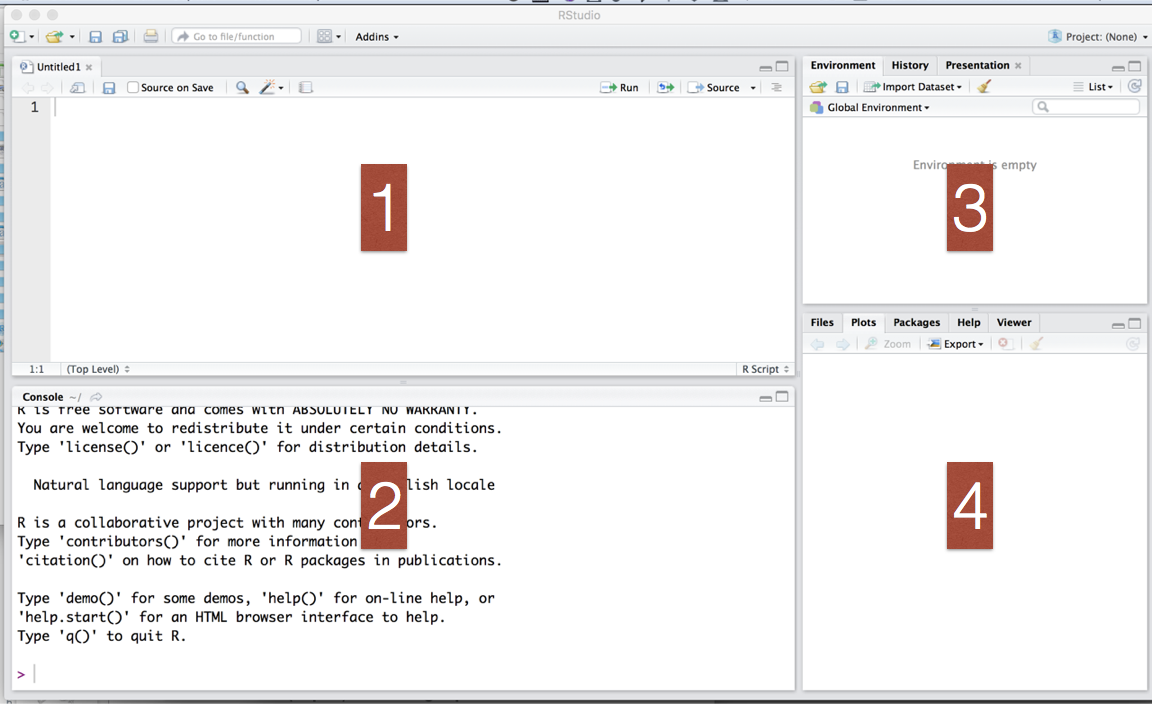
\includegraphics{img/rstudio-panes.png}

\hypertarget{executing-code-and-r-script-files}{%
\subsubsection*{Executing code and R script files}\label{executing-code-and-r-script-files}}
\addcontentsline{toc}{subsubsection}{Executing code and R script files}

You can start coding by typing commands in the Console panel. This window is also where the output will appear. Because this window is used for so many things it often fills up quickly --- and so, if you are doing anything involving a large number of steps, it is often easiest to type them in a script first.

You can create a new script by clicking on the ``File'' menu and selecting ``New File'' then ``R Script''. A script is a collection of commands that you can save and run again later. To run a command, click in a given line or highlight the text and hit \texttt{Ctrl+Enter}, or click the ``Run'' button at the top of the script window. You can save your scripts for later use.

Also very useful are the fact that in the main R Console window, the up and down-arrow on the key-board can be used to scroll through previously entered lines in R, and that \texttt{history()} will open a window of previously entered commands (which we'll see below after entering some). If the font in this R Console is too small, or if you dislike the color or font, you can change it by selecting ``Global Options'' under the ``Tools'' menu and clicking on the ``Appearance'' tab in the pop up window.

\hypertarget{rmarkdown}{%
\subsection*{RMarkdown}\label{rmarkdown}}
\addcontentsline{toc}{subsection}{RMarkdown}

Markdown is a particular type of markup language. Markup languages are designed to produce documents from plain text. Some of you may be familiar with LaTeX, another (less human friendly) markup language for creating pdf documents. LaTeX gives you much greater control, but it is restricted to pdf and has a much greater learning curve.

Markdown is becoming a standard and many websites will generate HTML from Markdown (e.g.~GitHub, Stack Overflow, reddit, \ldots). It is also relatively easy:

\begin{verbatim}
*italic*
**bold**
# Header 1
## Header 2
### Header 3
- List item 1
- List item 2
    - item 2a
    - item 2b
1. Numbered list item 1
1. Numbered list item 2
    - item 2a
    - item 2b
\end{verbatim}

Have a look at RStudio's \href{https://www.rstudio.com/resources/cheatsheets/}{RMarkdown cheat sheet}.

\begin{figure}
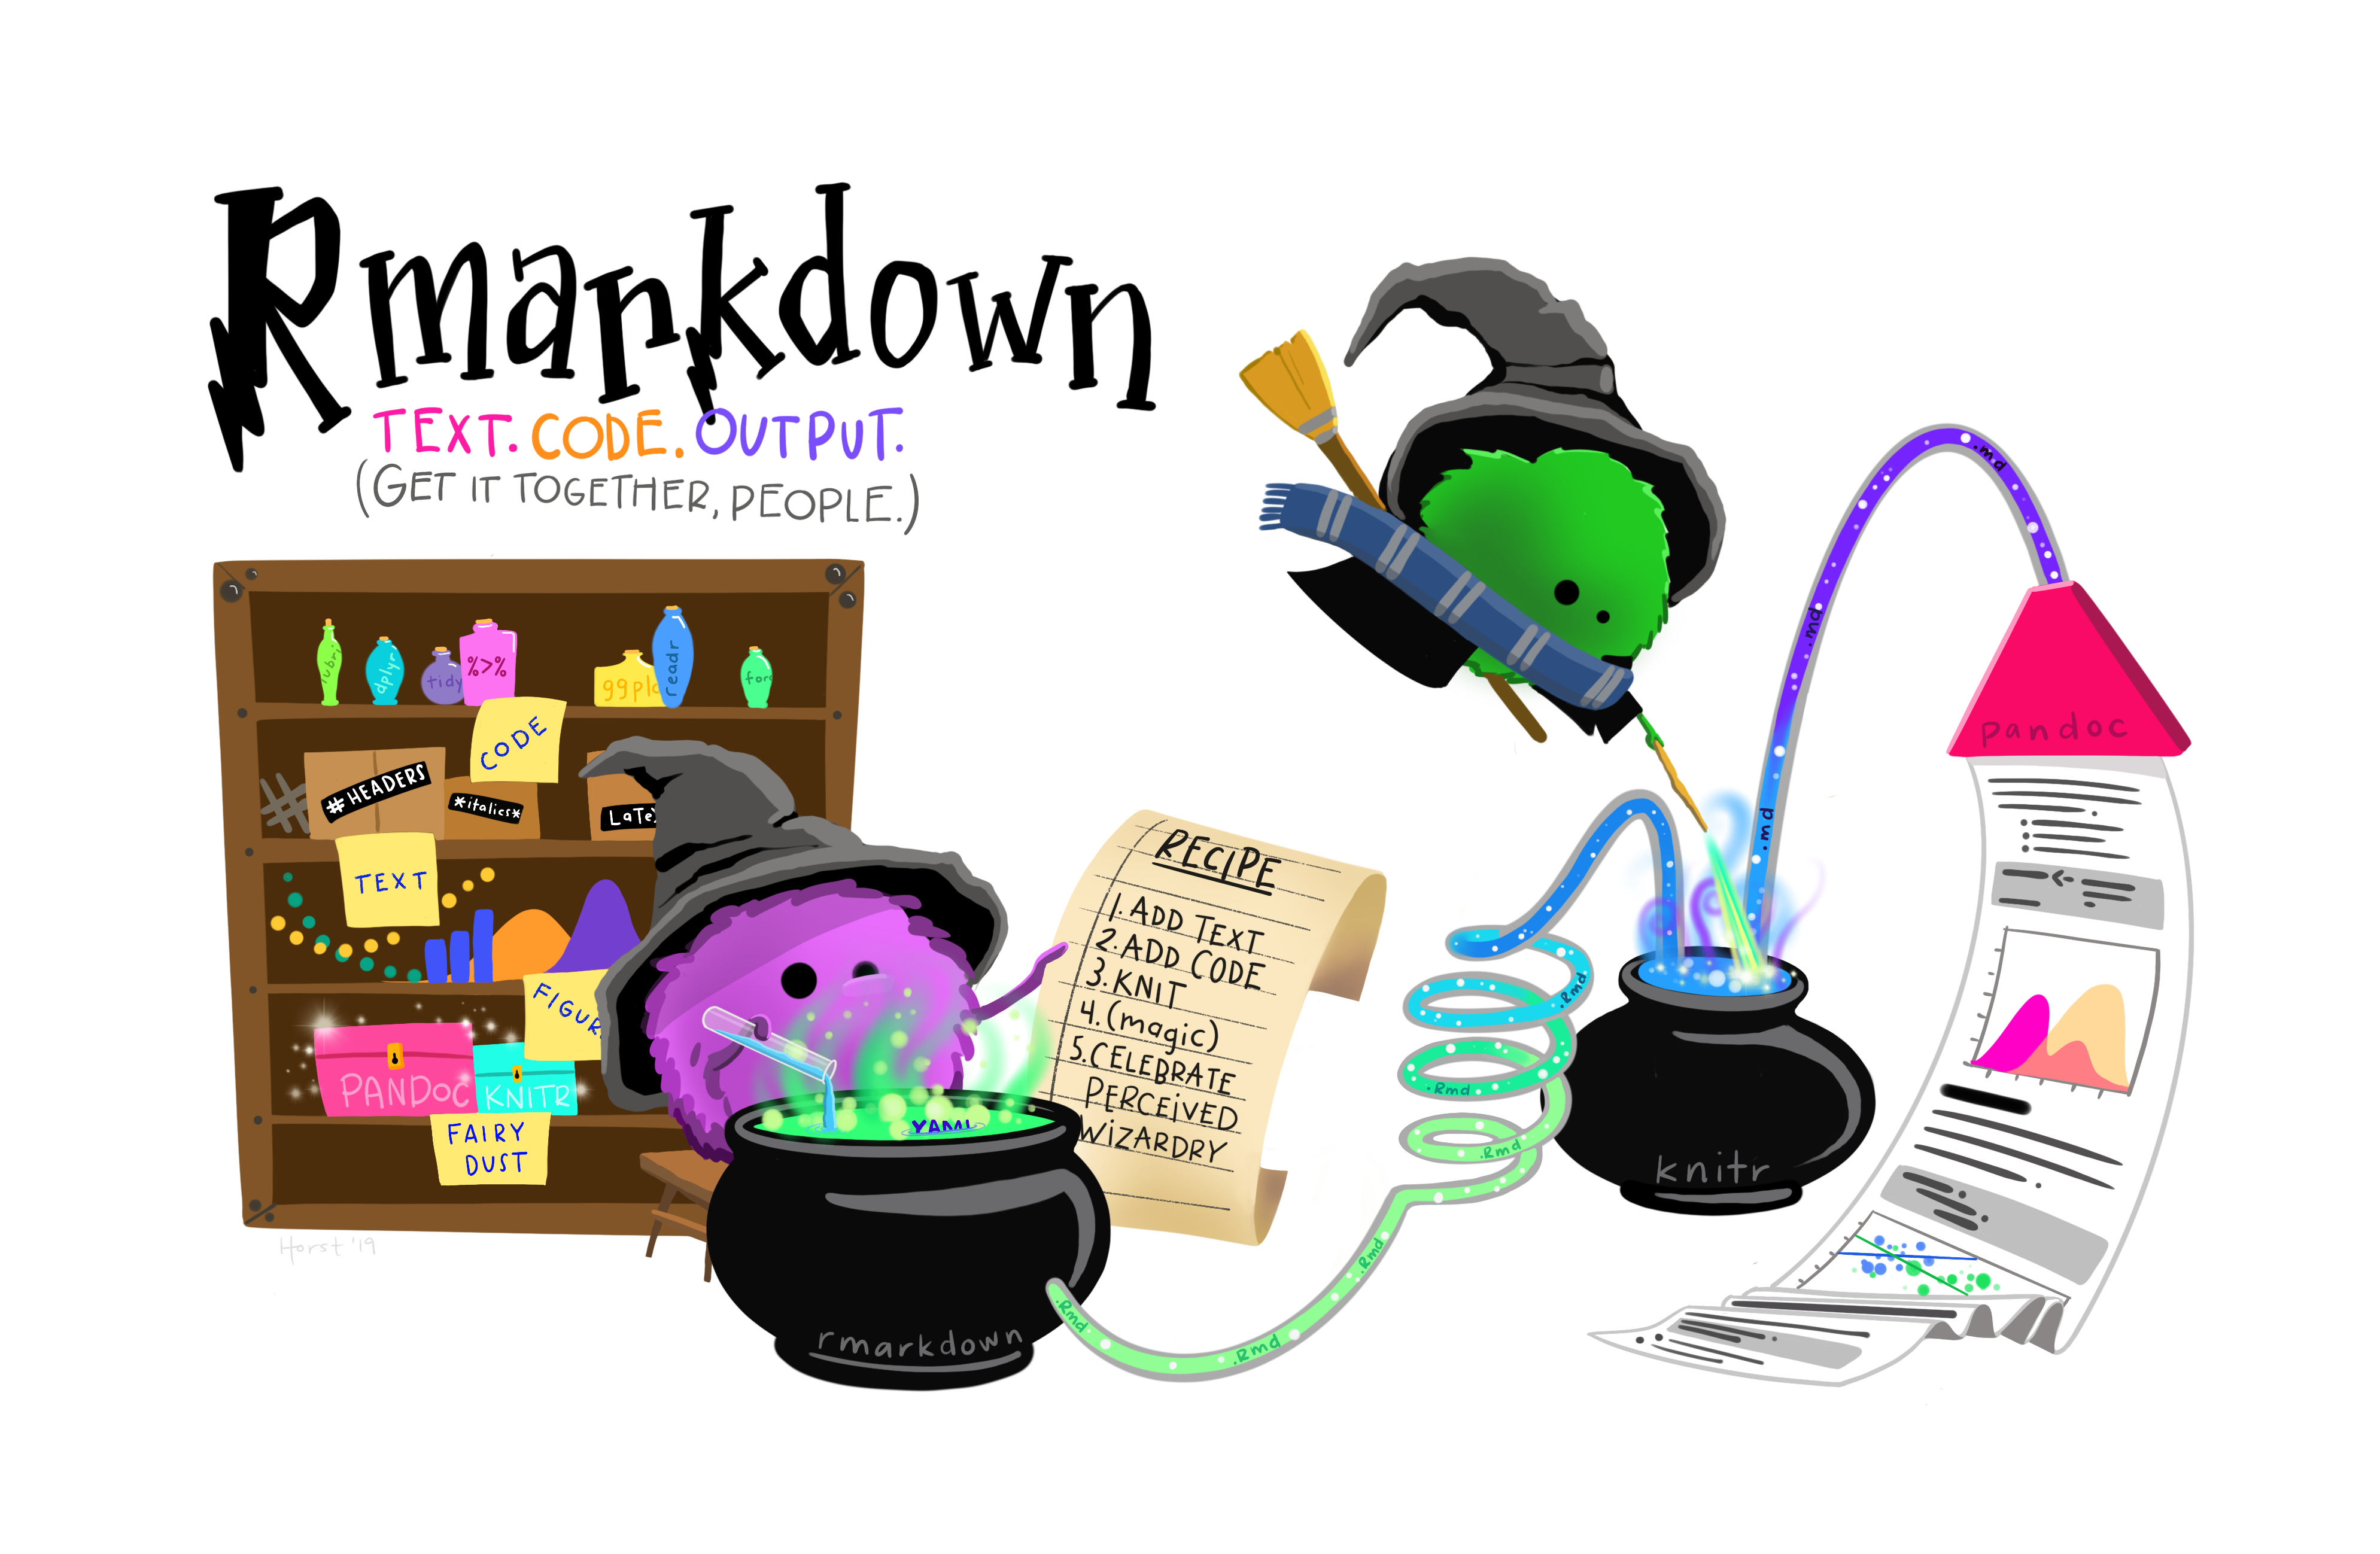
\includegraphics[width=55.24in]{img/rmarkdown_wizards} \caption{Artwork by allison horst}\label{fig:unnamed-chunk-1}
\end{figure}

\textbf{RMarkdown} is an authoring format that enables easy creation of dynamic documents, presentations, and reports from R. It combines markdown syntax with embedded R code chunks that are run so their output can be included in the final document.

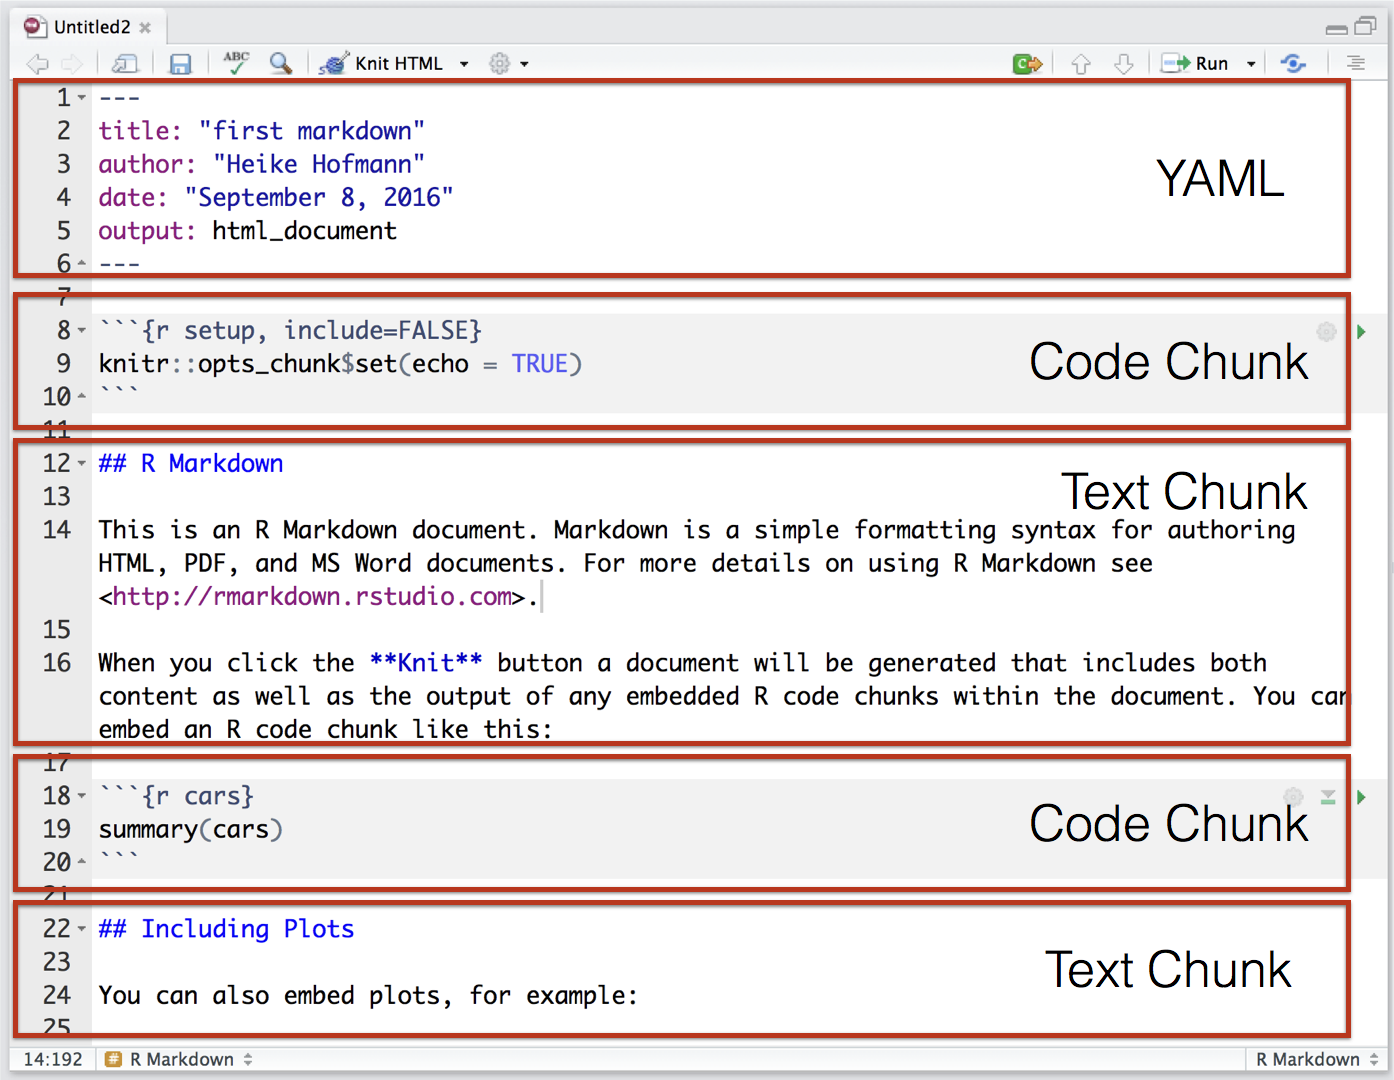
\includegraphics[width=19.36in]{img/rmarkdown}

Most importantly, RMarkdown creates fully reproducible reports since each time you knit the analysis is run from the beginning, encouraging transparency. Collaborators (including your future self) will thank you for integrating your analysis and report.

\hypertarget{exercise-create-your-first-rmarkdown.}{%
\subsubsection*{Exercise: Create your first Rmarkdown.}\label{exercise-create-your-first-rmarkdown.}}
\addcontentsline{toc}{subsubsection}{Exercise: Create your first Rmarkdown.}

\begin{enumerate}
\def\labelenumi{\arabic{enumi}.}
\tightlist
\item
  Open RStudio, create a new project.
\item
  Create a new RMarkdown file and knit it.
\item
  Make changes to the markdown formatting and knit again (use the \href{https://www.rstudio.com/resources/cheatsheets/}{RMarkdown cheat sheet})
\item
  If you feel adventurous, change some of the R code and knit again.
\end{enumerate}

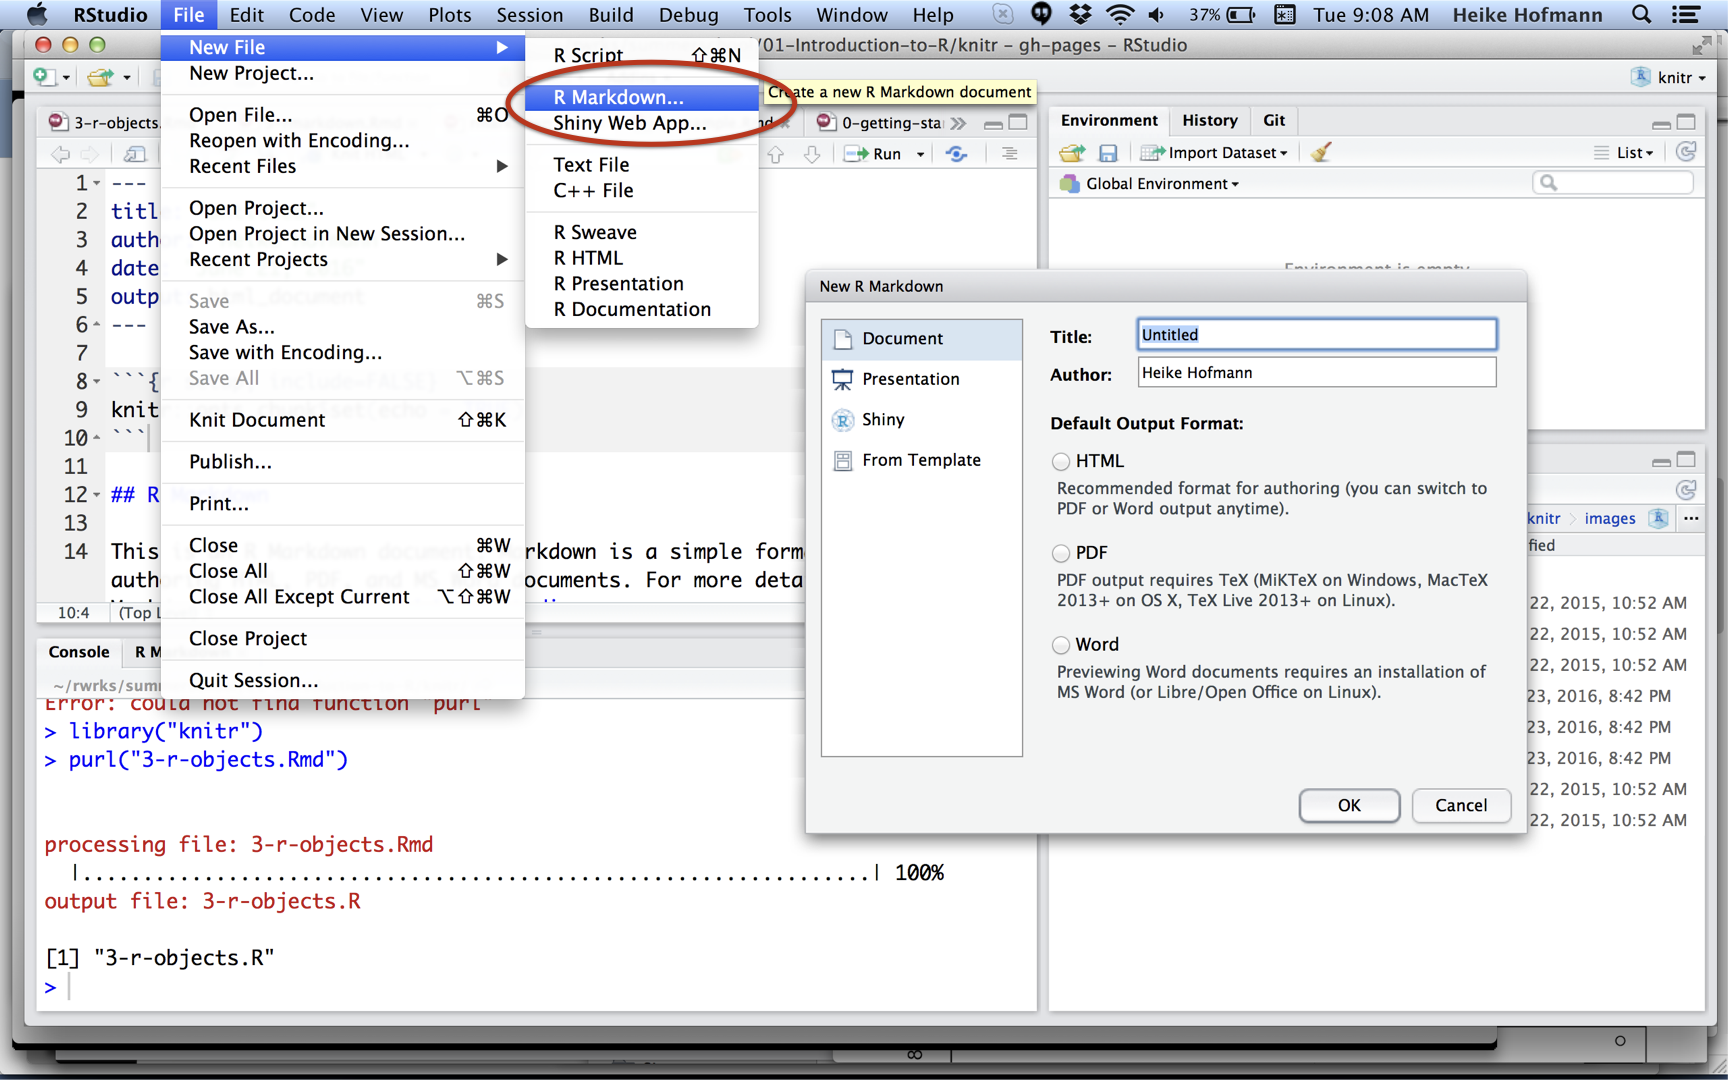
\includegraphics[width=24in]{img/hello-rmarkdown}

\hypertarget{objects}{%
\section{Objects}\label{objects}}

At the heart of R are the various objects that you enter. An object could be data (in the form of a single value, a vector, a matrix, an array, a list, or a data frame) or a function that you created. Objects are created by assigning a value to the objects name using either \texttt{\textless{}-} or \texttt{=}. For example

\begin{Shaded}
\begin{Highlighting}[]
\NormalTok{x }\OtherTok{\textless{}{-}} \DecValTok{3}
\end{Highlighting}
\end{Shaded}

All R statements where you create objects, \textbf{assignment statements}, have the same form:

\begin{Shaded}
\begin{Highlighting}[]
\NormalTok{object\_name }\OtherTok{\textless{}{-}}\NormalTok{ value}
\end{Highlighting}
\end{Shaded}

When reading that code say ``object name gets value'' in your head.

You will make lots of assignments, and \texttt{\textless{}-} is a pain to type. You can save time with \textbf{RStudio's keyboard shortcut: Alt + -} (the minus sign). Notice that RStudio automatically surrounds \texttt{\textless{}-} with spaces, which is a good code formatting practice. Code is miserable to read on a good day, so giveyoureyesabreak and use spaces.

If you run \texttt{x\ \textless{}-\ 3} in your local console (at the \texttt{\textgreater{}} prompt), R will only give you another prompt. This is because you merely assigned the value; you didn't ask R to do anything with it. Typing

\begin{Shaded}
\begin{Highlighting}[]
\NormalTok{x}
\end{Highlighting}
\end{Shaded}

\begin{verbatim}
## [1] 3
\end{verbatim}

will now return the number 3, the value of \texttt{x}. R is case sensitive, so entering

\begin{Shaded}
\begin{Highlighting}[]
\NormalTok{X }\OtherTok{\textless{}{-}} \DecValTok{5}
\NormalTok{X}
\end{Highlighting}
\end{Shaded}

\begin{verbatim}
## [1] 5
\end{verbatim}

will create a separate object. If you reassign an object, say:

\begin{Shaded}
\begin{Highlighting}[]
\NormalTok{X }\OtherTok{\textless{}{-}} \DecValTok{7}
\end{Highlighting}
\end{Shaded}

the original value is over-written. If you attempt to use the name of a built in function or constant (such as \texttt{c()}, \texttt{t()}, \texttt{t.test()}, or \texttt{pi()}) for one of your variable names, you will likely find that future work you are trying to do gives unexpected results. Notice in the name of \texttt{t.test()} that periods are allowed in names of objects. Other symbols (except numbers and letters) are not allowed.

Note that the up-arrow and \texttt{history()} will now show us the commands we entered previously. This set of all of your created objects (your Workspace) is not saved when you exit R, and this is purposeful: Attachment to your workspace indicates that you have a \textbf{non-reproducible} workflow. Any individual R process and the associated workspace is disposable and everything that really matters should be achieved through code that you save in your script.

\begin{figure}
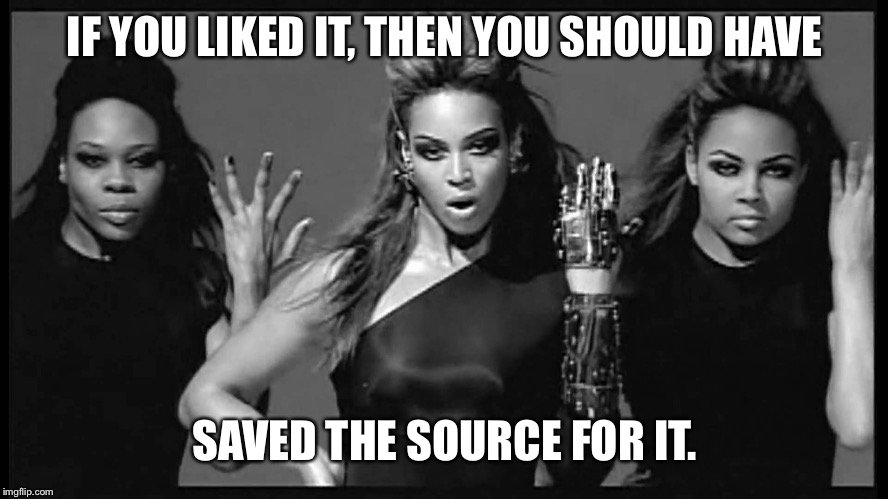
\includegraphics[width=12.33in]{img/if-you-liked-it-you-should-have-saved-the-source-for-it} \caption{ Image via Jenny Bryan's 'What They Forgot to Teach You About R'}\label{fig:unnamed-chunk-9}
\end{figure}

\hypertarget{data-types-in-r}{%
\subsection*{Data types in R}\label{data-types-in-r}}
\addcontentsline{toc}{subsection}{Data types in R}

\begin{itemize}
\tightlist
\item
  \textbf{logical}: boolean values

  \begin{itemize}
  \tightlist
  \item
    ex. \texttt{TRUE} and \texttt{FALSE}
  \end{itemize}
\item
  \textbf{double}: floating point numerical values (default numerical type)

  \begin{itemize}
  \tightlist
  \item
    ex. \texttt{1.335} and \texttt{7}
  \end{itemize}
\item
  \textbf{integer}: integer numerical values (indicated with an L)

  \begin{itemize}
  \tightlist
  \item
    ex. \texttt{7L} and \texttt{1:3}
  \end{itemize}
\item
  \textbf{character}: character string

  \begin{itemize}
  \tightlist
  \item
    ex. \texttt{"hello"}\\
  \end{itemize}
\item
  \textbf{lists}: 1d objects that can contain any combination of R objects
\item
  \& more, but we won't be focusing on those yet
\end{itemize}

\hypertarget{arithmetic-and-parentheses}{%
\section{Arithmetic and Parentheses}\label{arithmetic-and-parentheses}}

Using R can be a lot like using a calculator. All of the basic arithmetic operations work in R:

\begin{Shaded}
\begin{Highlighting}[]
\NormalTok{X }\SpecialCharTok{{-}}\NormalTok{ x}
\end{Highlighting}
\end{Shaded}

\begin{verbatim}
## [1] 4
\end{verbatim}

\begin{Shaded}
\begin{Highlighting}[]
\DecValTok{7} \SpecialCharTok{{-}} \DecValTok{3}
\end{Highlighting}
\end{Shaded}

\begin{verbatim}
## [1] 4
\end{verbatim}

will both return the value 4, one by performing the arithmetic on the objects, and the other on the numbers. The other basic mathematical operators are:

\begin{itemize}
\tightlist
\item
  \texttt{+} addition
\item
  \texttt{-} subtraction
\item
  \texttt{*} multiplication
\item
  \texttt{/} division
\item
  \texttt{\^{}} exponentiation
\item
  \texttt{\%*\%} matrix multiplication
\end{itemize}

R will often try to do the ``common-sense'' thing when using arithmetic arguments. For example, if \texttt{Y} is a vector or matrix of values, then \texttt{Y\ +\ 4} will add \texttt{4} to each of the values in \texttt{Y}. (So the vector \texttt{3,\ 2,\ 5} would become \texttt{7,\ 6,\ 9}).

Parentheses work as usual in mathematical statements, but they do not imply multiplication.

\begin{Shaded}
\begin{Highlighting}[]
\CommentTok{\#X(x+5)}
\NormalTok{X}\SpecialCharTok{*}\NormalTok{(x}\SpecialCharTok{+}\DecValTok{5}\NormalTok{)}
\end{Highlighting}
\end{Shaded}

\begin{verbatim}
## [1] 56
\end{verbatim}

Notice that the former returns an error about looking for a function called \texttt{X}, while the latter does the arithmetic to return the value \texttt{40}.

The other use of parentheses in R are to indicate that you attempting to run a function, and, if the function has any options it will contain those. The command:

\begin{Shaded}
\begin{Highlighting}[]
\FunctionTok{rnorm}\NormalTok{(}\DecValTok{10}\NormalTok{)}
\end{Highlighting}
\end{Shaded}

\begin{verbatim}
##  [1] -0.95996508  0.02171223  0.81844349  0.52626597  2.76736701  0.01628693
##  [7]  2.91319046 -1.42907179  0.12750983  0.20419454
\end{verbatim}

runs the function \texttt{rnorm()} with the argument \texttt{10}. In this case it is generating a random sample of 10 values from a normal distribution.

\hypertarget{help}{%
\section{Help!}\label{help}}

To see this, we could run the help function on that command.

\begin{Shaded}
\begin{Highlighting}[]
\FunctionTok{help}\NormalTok{(rnorm)}
\end{Highlighting}
\end{Shaded}

A shortcut, \texttt{?rnorm}, would also work.

Every help file in R begins with a brief description of the function (or group of functions) in question, followed by all of the possible options (a.k.a. Arguments) that you can provide. In this case the value \texttt{n} (the number of observations) is required. Notice that all of the other options are shown as being = some value -- this indicates the defaults those values take if you do not enter them. The sample we generated above thus has mean 0 and standard deviation 1.

Below the list of arguments are a brief summary of what the function does (called the \emph{Details}), a list of the \emph{Value} (or values) returned by running the function, the \emph{Source} of the algorithm, and general \emph{References} on the topic. \emph{See Also} is often the most useful part of the help for a function as it provides a list of related functions. Finally, there are some \emph{Examples} that you can cut and paste in to observe the function in action.

\hypertarget{functions}{%
\section{Functions}\label{functions}}

Functions are (most often) verbs, followed by what they will be applied to in parentheses:

\begin{Shaded}
\begin{Highlighting}[]
\FunctionTok{do\_this}\NormalTok{(to\_this)}
\FunctionTok{do\_that}\NormalTok{(to\_this, to\_that, with\_those)}
\end{Highlighting}
\end{Shaded}

It is always safest to enter the values of functions using the names of the arguments:

\begin{Shaded}
\begin{Highlighting}[]
\FunctionTok{rnorm}\NormalTok{(}\DecValTok{10}\NormalTok{, }\AttributeTok{sd =} \DecValTok{4}\NormalTok{)}
\end{Highlighting}
\end{Shaded}

\begin{verbatim}
##  [1]  1.1041604 -2.4408774  0.1893304 -2.6351240 -1.8391115  2.2828173
##  [7] -6.9364568 -5.2319864 -3.0551216  5.4756209
\end{verbatim}

rather than trusting that the argument you want happens to be first in the list:

\begin{Shaded}
\begin{Highlighting}[]
\FunctionTok{rnorm}\NormalTok{(}\DecValTok{10}\NormalTok{, }\DecValTok{4}\NormalTok{)}
\end{Highlighting}
\end{Shaded}

\begin{verbatim}
##  [1] 2.901461 5.012511 3.642010 2.329912 3.341805 3.801201 5.121462 3.820371
##  [9] 3.824450 4.874095
\end{verbatim}

Notice the former puts 4 in for the standard deviation, while the latter is putting it in for the second overall argument, the mean (as seen in the help file).

Note that these values we generated have not been saved as an object, and exist solely on the screen. To save the values we could have assigned the output of our function to an object.

\begin{Shaded}
\begin{Highlighting}[]
\NormalTok{normal.sample }\OtherTok{\textless{}{-}} \FunctionTok{rnorm}\NormalTok{(}\DecValTok{50}\NormalTok{)}
\NormalTok{normal.sample}
\end{Highlighting}
\end{Shaded}

\begin{verbatim}
##  [1] -1.35193126  1.58106587  0.89892238 -0.98692374 -2.19489135 -0.66274938
##  [7] -1.99435789 -0.75871439 -0.76360928  1.55226649 -0.66183804  0.55079659
## [13] -0.26950343  1.81811137  0.38366594  1.10882297 -0.74430439  1.44094003
## [19] -0.60807632  0.55699076 -0.55448268  0.30121418  0.04234729  0.29993612
## [25] -0.05719389  0.81856983 -1.00679132 -1.29156383 -0.23244611 -0.46500074
## [31]  0.80627995 -0.12040647 -1.21275214 -2.12957949  0.63944735 -0.89921133
## [37]  1.01528125  0.50202615  0.48329558  0.31986368  0.05283811 -2.06815539
## [43] -0.71354598 -0.59078981  0.63298780 -0.92026428  0.80324869  0.65404826
## [49] -0.82803953 -0.44314635
\end{verbatim}

A few common statistical functions include:

\begin{itemize}
\tightlist
\item
  \texttt{mean()} find the mean
\item
  \texttt{median()} find the median
\item
  \texttt{sd()} find the standard deviation
\item
  \texttt{var()} find the variance
\item
  \texttt{quantile()} find the quantiles (percentiles);

  \begin{itemize}
  \tightlist
  \item
    requires the data and the percentile you want
  \item
    e.g.~\texttt{quantile(normal.sample,\ .5)} is the median
  \end{itemize}
\item
  \texttt{max()} find the maximum
\item
  \texttt{min()} find the minimum
\item
  \texttt{summary()} find the 5-number summary
\item
  \texttt{hist()} construct a histogram
\item
  \texttt{boxplot()} construct a boxplot
\item
  \texttt{qqnorm()} construct a normal quantile-quantile plot
\item
  \texttt{qqline()} add the line to a normal quantile-quantile plot
\end{itemize}

Trying a few of these out (like \texttt{mean(normal.sample)}) will show us the descriptive statistics and basic graphs for a sample of size 50 from a normal population with mean 0 and standard deviation 1. (Using up arrow can make it quicker to try several in a row.)

As we will see in more detail later, it is possible to create your own functions by using the function function. This one creates a simple measure of skewness.

\begin{Shaded}
\begin{Highlighting}[]
\NormalTok{Skew }\OtherTok{\textless{}{-}} \ControlFlowTok{function}\NormalTok{(x)\{}
\NormalTok{    (}\FunctionTok{mean}\NormalTok{(x) }\SpecialCharTok{{-}} \FunctionTok{median}\NormalTok{(x))}\SpecialCharTok{/}\FunctionTok{sd}\NormalTok{(x)\}}
\end{Highlighting}
\end{Shaded}

Note that braces \texttt{\{\ \}} in R are used to group several separate commands together, and also occur when using programming commands like loops or if-then statements. They work the same as parentheses in arithmetic expressions.

After entering or new function, it works like any built in function, except that it appears in our objects list.

\begin{Shaded}
\begin{Highlighting}[]
\CommentTok{\# Skew}
\CommentTok{\# Skew()}
\FunctionTok{Skew}\NormalTok{(normal.sample)}
\end{Highlighting}
\end{Shaded}

\begin{verbatim}
## [1] 0.03119983
\end{verbatim}

There are also a number of mathematical functions as well. Ones common in statistical applications include:

\begin{itemize}
\tightlist
\item
  \texttt{sqrt()} square root
\item
  \texttt{exp()} exponent (e to the power)
\item
  \texttt{log()} the natural logarithm by default
\item
  \texttt{abs()} absolute values
\item
  \texttt{floor()} round down
\item
  \texttt{ceiling()} round up
\item
  \texttt{round()} round to the nearest (even if .5)
\end{itemize}

\hypertarget{vectors-matrices-and-arrays}{%
\section{Vectors, Matrices, and Arrays}\label{vectors-matrices-and-arrays}}

The output from \texttt{rnorm()} is different from the \texttt{X} and \texttt{x} we created as it contains more than just a single value - they are vectors. While we can think of them as vectors in the mathematical sense, we can also think of a vector as simply listing the values of a variable.

Vectors in R are created using the \texttt{c()} function (as in concatonate). Thus,

\begin{Shaded}
\begin{Highlighting}[]
\NormalTok{Y }\OtherTok{\textless{}{-}} \FunctionTok{c}\NormalTok{(}\DecValTok{3}\NormalTok{, }\DecValTok{2}\NormalTok{, }\DecValTok{5}\NormalTok{)}
\NormalTok{Y}
\end{Highlighting}
\end{Shaded}

\begin{verbatim}
## [1] 3 2 5
\end{verbatim}

\begin{Shaded}
\begin{Highlighting}[]
\NormalTok{Y }\SpecialCharTok{+} \DecValTok{4}
\end{Highlighting}
\end{Shaded}

\begin{verbatim}
## [1] 7 6 9
\end{verbatim}

\begin{Shaded}
\begin{Highlighting}[]
\NormalTok{Y }\SpecialCharTok{*} \DecValTok{2}
\end{Highlighting}
\end{Shaded}

\begin{verbatim}
## [1]  6  4 10
\end{verbatim}

creates a vector of length three (and we can verify that arithmetic works on it componentwise). Given two vectors arithmetic is also done componentwise:

\begin{Shaded}
\begin{Highlighting}[]
\NormalTok{Z }\OtherTok{\textless{}{-}} \FunctionTok{c}\NormalTok{(}\DecValTok{1}\NormalTok{, }\DecValTok{2}\NormalTok{, }\DecValTok{3}\NormalTok{)}
\NormalTok{Y }\SpecialCharTok{+}\NormalTok{ Z}
\end{Highlighting}
\end{Shaded}

\begin{verbatim}
## [1] 4 4 8
\end{verbatim}

\begin{Shaded}
\begin{Highlighting}[]
\NormalTok{Y }\SpecialCharTok{*}\NormalTok{ Z}
\end{Highlighting}
\end{Shaded}

\begin{verbatim}
## [1]  3  4 15
\end{verbatim}

Other functions are also evaluated component-wise (if possible):

\begin{Shaded}
\begin{Highlighting}[]
\FunctionTok{sqrt}\NormalTok{(Z)}
\end{Highlighting}
\end{Shaded}

\begin{verbatim}
## [1] 1.000000 1.414214 1.732051
\end{verbatim}

Multiple vectors can be combined together by using the \texttt{c()} function:

\begin{Shaded}
\begin{Highlighting}[]
\NormalTok{YandZ }\OtherTok{\textless{}{-}} \FunctionTok{c}\NormalTok{(Y, Z)}
\NormalTok{YandZ}
\end{Highlighting}
\end{Shaded}

\begin{verbatim}
## [1] 3 2 5 1 2 3
\end{verbatim}

However, when asked to combine vectors of two different types, R will try to force them to be of the same type:

\begin{Shaded}
\begin{Highlighting}[]
\NormalTok{nums }\OtherTok{\textless{}{-}} \FunctionTok{c}\NormalTok{(}\DecValTok{1}\NormalTok{, }\DecValTok{2}\NormalTok{, }\DecValTok{3}\NormalTok{)}
\NormalTok{nums}
\end{Highlighting}
\end{Shaded}

\begin{verbatim}
## [1] 1 2 3
\end{verbatim}

\begin{Shaded}
\begin{Highlighting}[]
\NormalTok{lttrs }\OtherTok{\textless{}{-}} \FunctionTok{c}\NormalTok{(}\StringTok{"a"}\NormalTok{, }\StringTok{"b"}\NormalTok{, }\StringTok{"c"}\NormalTok{)}
\NormalTok{lttrs}
\end{Highlighting}
\end{Shaded}

\begin{verbatim}
## [1] "a" "b" "c"
\end{verbatim}

\begin{Shaded}
\begin{Highlighting}[]
\FunctionTok{c}\NormalTok{(nums, lttrs)}
\end{Highlighting}
\end{Shaded}

\begin{verbatim}
## [1] "1" "2" "3" "a" "b" "c"
\end{verbatim}

\begin{Shaded}
\begin{Highlighting}[]
\CommentTok{\# c(nums, lttrs) + 2}
\end{Highlighting}
\end{Shaded}

Once we have our desired vector, an element in the vector can be referred to by using square brackets:

\begin{Shaded}
\begin{Highlighting}[]
\NormalTok{YandZ[}\DecValTok{2}\NormalTok{]}
\end{Highlighting}
\end{Shaded}

\begin{verbatim}
## [1] 2
\end{verbatim}

\begin{Shaded}
\begin{Highlighting}[]
\NormalTok{YandZ[}\DecValTok{2}\SpecialCharTok{:}\DecValTok{4}\NormalTok{]}
\end{Highlighting}
\end{Shaded}

\begin{verbatim}
## [1] 2 5 1
\end{verbatim}

\begin{Shaded}
\begin{Highlighting}[]
\NormalTok{YandZ[}\FunctionTok{c}\NormalTok{(}\DecValTok{1}\NormalTok{, }\DecValTok{4}\SpecialCharTok{:}\DecValTok{6}\NormalTok{)]}
\end{Highlighting}
\end{Shaded}

\begin{verbatim}
## [1] 3 1 2 3
\end{verbatim}

By using the \texttt{c()} function, and the \texttt{:} to indicate a sequence of numbers, you can quickly refer to the particular portion of the data you are concerned with.

Matrices (two-dimensional) and arrays (more than two dimensions) work similarly - they use brackets to find particular values, and all the values in an array or matrix must be of the same type (e.g.~numeric, character, or factor). In the case of matrices, the first values in the brackets indicates the desired rows, and the ones after the comma indicate the desired columns.

\begin{Shaded}
\begin{Highlighting}[]
\NormalTok{Xmat }\OtherTok{\textless{}{-}} \FunctionTok{matrix}\NormalTok{(}\FunctionTok{c}\NormalTok{(}\DecValTok{3}\NormalTok{, }\DecValTok{2}\NormalTok{, }\DecValTok{5}\NormalTok{, }\DecValTok{1}\NormalTok{, }\DecValTok{2}\NormalTok{, }\DecValTok{3}\NormalTok{), }
               \AttributeTok{ncol =} \DecValTok{3}\NormalTok{, }\AttributeTok{byrow =} \ConstantTok{TRUE}\NormalTok{)}
\NormalTok{Xmat}
\end{Highlighting}
\end{Shaded}

\begin{verbatim}
##      [,1] [,2] [,3]
## [1,]    3    2    5
## [2,]    1    2    3
\end{verbatim}

\begin{Shaded}
\begin{Highlighting}[]
\NormalTok{Ymat }\OtherTok{\textless{}{-}} \FunctionTok{rbind}\NormalTok{(Y, Z)}
\NormalTok{Ymat}
\end{Highlighting}
\end{Shaded}

\begin{verbatim}
##   [,1] [,2] [,3]
## Y    3    2    5
## Z    1    2    3
\end{verbatim}

\begin{Shaded}
\begin{Highlighting}[]
\NormalTok{Xmat[}\DecValTok{1}\NormalTok{, }\DecValTok{2}\SpecialCharTok{:}\DecValTok{3}\NormalTok{]}
\end{Highlighting}
\end{Shaded}

\begin{verbatim}
## [1] 2 5
\end{verbatim}

\begin{Shaded}
\begin{Highlighting}[]
\NormalTok{Zmat }\OtherTok{\textless{}{-}} \FunctionTok{cbind}\NormalTok{(nums, lttrs)}
\NormalTok{Zmat}
\end{Highlighting}
\end{Shaded}

\begin{verbatim}
##      nums lttrs
## [1,] "1"  "a"  
## [2,] "2"  "b"  
## [3,] "3"  "c"
\end{verbatim}

In the above code, \texttt{matrix()} is the function to form a vector into a matrix, \texttt{rbind()} places multiple vectors (or matrices) side-by-side as the rows of a new matrix (if the dimensions match), and \texttt{cbind()} does the same for columns.

\hypertarget{data-frames-lists-and-attributes}{%
\section{Data Frames, Lists, and Attributes}\label{data-frames-lists-and-attributes}}

In many cases the data set we wish to analyze will not have all of the rows or columns in the same format. This type of data is stored in R as a \textbf{data frame}. A data frame is a rectangular collection of variables (in the columns) and observations (in the rows).

\texttt{scdata.txt} is one such data set, and it can be found in the course materials (its description is found in \texttt{scdata.pdf}). The data can be read in using code similar to the below (assuming a similar file structure).

\begin{Shaded}
\begin{Highlighting}[]
\NormalTok{sctable }\OtherTok{\textless{}{-}}\NormalTok{ readr}\SpecialCharTok{::}\FunctionTok{read\_table}\NormalTok{(}\StringTok{"data/scdata.txt"}\NormalTok{)}
\end{Highlighting}
\end{Shaded}

\begin{verbatim}
## 
## -- Column specification --------------------------------------------------------
## cols(
##   .default = col_double(),
##   County = col_character(),
##   Region = col_character()
## )
## i Use `spec()` for the full column specifications.
\end{verbatim}

\hypertarget{inspecting-objects}{%
\subsection*{Inspecting Objects}\label{inspecting-objects}}
\addcontentsline{toc}{subsection}{Inspecting Objects}

To inspect the data without needing to print out the entire data set, we can try out the following commands:

\begin{itemize}
\tightlist
\item
  \texttt{head()}
\item
  \texttt{tail()}
\item
  \texttt{summary()}
\item
  \texttt{str()}
\item
  \texttt{dim()}
\end{itemize}

For example, use \texttt{head()} and \texttt{tail()} to see the first and last rows. This lets you check the variable names as well as the number of observations successfully read in.

\begin{Shaded}
\begin{Highlighting}[]
\FunctionTok{head}\NormalTok{(sctable)}
\end{Highlighting}
\end{Shaded}

\begin{verbatim}
## # A tibble: 6 x 27
##   County Region Births Death InfMort Minor~1 Over65 PopChng PopDens Urban Income
##   <chr>  <chr>   <dbl> <dbl>   <dbl>   <dbl>  <dbl>   <dbl>   <dbl> <dbl>  <dbl>
## 1 Abbev~ Upsta~   12.5  10.3    15.1    31.7   14.7     9.7    51.5  23.4  32635
## 2 Aiken  Midla~   12.1   9.8     9.6    28.6   12.8    17.8   133.   60.9  37889
## 3 Allen~ LowCo~   14.8  12.1    18.5    72.6   12.7    -4.4    27.5  59    20898
## 4 Ander~ Upsta~   13    10.7    10.3    18.4   13.7    14.2   231.   58.3  36807
## 5 Bambe~ Midla~   11.5   9.9    21.7    63.5   13.9    -1.4    42.4  45.7  24007
## 6 Barnw~ Midla~   14    10.9    21.4    44.8   12.6    15.7    42.8  14.9  28591
## # ... with 16 more variables: ConsInc <dbl>, FarmInc <dbl>, ManIncom <dbl>,
## #   RetInc <dbl>, FdStmps <dbl>, MoblHms <dbl>, NoCar <dbl>, PlumProb <dbl>,
## #   PoorChild <dbl>, Unemp <dbl>, Coll4 <dbl>, Crime <dbl>, HSGrad <dbl>,
## #   JuvDel <dbl>, MVDeath <dbl>, SchlSpnd <dbl>, and abbreviated variable name
## #   1: Minority
\end{verbatim}

\begin{Shaded}
\begin{Highlighting}[]
\FunctionTok{tail}\NormalTok{(sctable)}
\end{Highlighting}
\end{Shaded}

\begin{verbatim}
## # A tibble: 6 x 27
##   County Region Births Death InfMort Minor~1 Over65 PopChng PopDens Urban Income
##   <chr>  <chr>   <dbl> <dbl>   <dbl>   <dbl>  <dbl>   <dbl>   <dbl> <dbl>  <dbl>
## 1 Saluda Midla~   11.2  11.3     4.7    34.2   14.5    16.7    42.5  18.7  35774
## 2 Spart~ Upsta~   13.1   9.8     7.9    24.9   12.5    11.9   313.   64.8  37579
## 3 Sumter Midla~   15.6   8.9     8.5    50     11.2     3.3   157.   62.1  33278
## 4 Union  Upsta~   10.7  13.2    12.8    32.2   15.6    -1.5    58.1  35.7  31441
## 5 Willi~ Peedee   12.6  11.8     8.8    67.3   13       1.1    39.8  15.1  24214
## 6 York   Upsta~   13.4   7.7     7.6    22.7   10.4    25.2   241.   64.3  44539
## # ... with 16 more variables: ConsInc <dbl>, FarmInc <dbl>, ManIncom <dbl>,
## #   RetInc <dbl>, FdStmps <dbl>, MoblHms <dbl>, NoCar <dbl>, PlumProb <dbl>,
## #   PoorChild <dbl>, Unemp <dbl>, Coll4 <dbl>, Crime <dbl>, HSGrad <dbl>,
## #   JuvDel <dbl>, MVDeath <dbl>, SchlSpnd <dbl>, and abbreviated variable name
## #   1: Minority
\end{verbatim}

\hypertarget{extracting-parts-of-objects}{%
\subsection*{Extracting parts of objects}\label{extracting-parts-of-objects}}
\addcontentsline{toc}{subsection}{Extracting parts of objects}

For object \texttt{x}, we can extract parts in the following manner (\texttt{rows} and \texttt{columns} are vectors of indices):

\begin{Shaded}
\begin{Highlighting}[]
\NormalTok{x}\SpecialCharTok{$}\NormalTok{variable}
\NormalTok{x[, }\StringTok{"variable"}\NormalTok{]}
\NormalTok{x[rows, columns]}
\NormalTok{x[}\DecValTok{1}\SpecialCharTok{:}\DecValTok{5}\NormalTok{, }\DecValTok{2}\SpecialCharTok{:}\DecValTok{3}\NormalTok{]}
\NormalTok{x[}\FunctionTok{c}\NormalTok{(}\DecValTok{1}\NormalTok{,}\DecValTok{5}\NormalTok{,}\DecValTok{6}\NormalTok{), }\FunctionTok{c}\NormalTok{(}\StringTok{"County"}\NormalTok{, }\StringTok{"Region"}\NormalTok{)]}
\NormalTok{x}\SpecialCharTok{$}\NormalTok{variable[rows]}
\end{Highlighting}
\end{Shaded}

Many of these extraction methods access the rows and columns of a data frame by treating it similarly to a matrix:

\begin{Shaded}
\begin{Highlighting}[]
\NormalTok{County1 }\OtherTok{\textless{}{-}}\NormalTok{ sctable[}\DecValTok{1}\NormalTok{, ]}
\NormalTok{Birth.Death }\OtherTok{\textless{}{-}}\NormalTok{ sctable[ , }\DecValTok{3}\SpecialCharTok{:}\DecValTok{4}\NormalTok{]}
\end{Highlighting}
\end{Shaded}

This simplicity sometimes causes trouble though. While \texttt{Birth.Death} may look on the screen like it is a matrix, it is still a data frame and many functions which use matrix operations (like matrix multiplication) will give an error. The \texttt{attributes()} function will show us the true status of our object (it returns \texttt{NULL} for a numeric vector and the dimensions if a matrix):

\begin{Shaded}
\begin{Highlighting}[]
\NormalTok{Birth.Death}
\end{Highlighting}
\end{Shaded}

\begin{verbatim}
## # A tibble: 46 x 2
##    Births Death
##     <dbl> <dbl>
##  1   12.5  10.3
##  2   12.1   9.8
##  3   14.8  12.1
##  4   13    10.7
##  5   11.5   9.9
##  6   14    10.9
##  7   15.8   7.8
##  8   14.4   6.6
##  9   11.5  11.1
## 10   14.5   8.5
## # ... with 36 more rows
\end{verbatim}

\begin{Shaded}
\begin{Highlighting}[]
\FunctionTok{attributes}\NormalTok{(Birth.Death)}
\end{Highlighting}
\end{Shaded}

\begin{verbatim}
## $names
## [1] "Births" "Death" 
## 
## $row.names
##  [1]  1  2  3  4  5  6  7  8  9 10 11 12 13 14 15 16 17 18 19 20 21 22 23 24 25
## [26] 26 27 28 29 30 31 32 33 34 35 36 37 38 39 40 41 42 43 44 45 46
## 
## $class
## [1] "tbl_df"     "tbl"        "data.frame"
\end{verbatim}

\begin{Shaded}
\begin{Highlighting}[]
\NormalTok{BD.matrix }\OtherTok{\textless{}{-}} \FunctionTok{as.matrix}\NormalTok{(Birth.Death)}
\FunctionTok{attributes}\NormalTok{(BD.matrix)}
\end{Highlighting}
\end{Shaded}

\begin{verbatim}
## $dim
## [1] 46  2
## 
## $dimnames
## $dimnames[[1]]
## NULL
## 
## $dimnames[[2]]
## [1] "Births" "Death"
\end{verbatim}

The \texttt{\$} is used to access whatever corresponds to an entry in the names attribute:

\begin{Shaded}
\begin{Highlighting}[]
\NormalTok{Birth.Death}\SpecialCharTok{$}\NormalTok{Births}
\end{Highlighting}
\end{Shaded}

\begin{verbatim}
##  [1] 12.5 12.1 14.8 13.0 11.5 14.0 15.8 14.4 11.5 14.5 13.3 12.3 12.1 12.3 13.0
## [16] 12.4 15.6 12.9 10.3 12.8 15.3 12.7 14.0 12.6 13.9 12.7 14.3 12.8 12.2 11.6
## [31] 12.9 14.0  7.6 13.8 11.9 12.5 11.7 13.8 11.2 13.3 11.2 13.1 15.6 10.7 12.6
## [46] 13.4
\end{verbatim}

This is particularly useful when trying to access a portion of the output of a function for later use. For example, later we will see a method of doing statistical inference called the t-test. In R, this is performed by the function \texttt{t.test()} which can create a great deal of output on the screen.

\begin{Shaded}
\begin{Highlighting}[]
\FunctionTok{t.test}\NormalTok{(normal.sample)}
\end{Highlighting}
\end{Shaded}

\begin{verbatim}
## 
##  One Sample t-test
## 
## data:  normal.sample
## t = -1.0317, df = 49, p-value = 0.3073
## alternative hypothesis: true mean is not equal to 0
## 95 percent confidence interval:
##  -0.4284537  0.1377616
## sample estimates:
## mean of x 
## -0.145346
\end{verbatim}

If you only want the part called the ``p-value'' for later use we can pull that out of the output.

\begin{Shaded}
\begin{Highlighting}[]
\NormalTok{t.out }\OtherTok{\textless{}{-}} \FunctionTok{t.test}\NormalTok{(normal.sample)}
\FunctionTok{attributes}\NormalTok{(t.out)}
\end{Highlighting}
\end{Shaded}

\begin{verbatim}
## $names
##  [1] "statistic"   "parameter"   "p.value"     "conf.int"    "estimate"   
##  [6] "null.value"  "stderr"      "alternative" "method"      "data.name"  
## 
## $class
## [1] "htest"
\end{verbatim}

\begin{Shaded}
\begin{Highlighting}[]
\NormalTok{t.out}\SpecialCharTok{$}\NormalTok{p.value}
\end{Highlighting}
\end{Shaded}

\begin{verbatim}
## [1] 0.3072755
\end{verbatim}

We could then save the resulting value as part of a vector or matrix of other p-values, for example.

The \texttt{\$} is also used to access named parts of lists, which we will see can be used to store a variety of kinds of information in a single object.

\hypertarget{packages}{%
\section{Packages}\label{packages}}

The ability to ``easily'' write functions in R has lead to an explosion of procedures that researchers have written and made available to the public, typically as an R package. An R package is a collection of functions, data, and documentation that extends the capabilities of base R. Using packages is key to the successful use of R. For example, the \textbf{MASS} package contains all of the functions corresponding to the Springer text \emph{Modern Applied Statistics with S} by Venables and Ripley.

While some of these are automatically included with the basic installation of R, most are not and can installed with the \texttt{install.packages()} function.

\begin{Shaded}
\begin{Highlighting}[]
\FunctionTok{install.packages}\NormalTok{(}\StringTok{"package\_name"}\NormalTok{)}
\end{Highlighting}
\end{Shaded}

When you run the code to install a package on your own computer, R will download the packages from CRAN and install them on to your computer.

If you have problems installing, make sure that you are connected to the internet, and that \url{https://cloud.r-project.org/} isn't blocked by your firewall or proxy.

You will not be able to use the functions, objects, and help files in a package until you load it with \texttt{library()}.

\begin{Shaded}
\begin{Highlighting}[]
\FunctionTok{library}\NormalTok{(package\_name)}
\end{Highlighting}
\end{Shaded}

The command \texttt{library()} is used to activate a downloaded package and give access to all of its functions and must be done once per session.

\begin{Shaded}
\begin{Highlighting}[]
\CommentTok{\# help(fractions)}
\FunctionTok{library}\NormalTok{(MASS)}
\FunctionTok{help}\NormalTok{(fractions)}
\FunctionTok{fractions}\NormalTok{(}\FloatTok{0.5}\NormalTok{)}
\end{Highlighting}
\end{Shaded}

\begin{verbatim}
## [1] 1/2
\end{verbatim}

\begin{Shaded}
\begin{Highlighting}[]
\FunctionTok{fractions}\NormalTok{(pi)}
\end{Highlighting}
\end{Shaded}

\begin{verbatim}
## [1] 4272943/1360120
\end{verbatim}

\begin{Shaded}
\begin{Highlighting}[]
\DecValTok{4272943}\SpecialCharTok{/}\DecValTok{1360120}
\end{Highlighting}
\end{Shaded}

\begin{verbatim}
## [1] 3.141593
\end{verbatim}

\hypertarget{statistical-analysis}{%
\chapter{Statistical Analysis}\label{statistical-analysis}}

There are a huge variety of statistical tests built in to R for analyzing data. In many cases the same function will perform several different tests and confidence intervals, and produce a large amount of output. We provide examples of many of these functions below, including some that are part of other packages, and others that are custom written functions.

\begin{Shaded}
\begin{Highlighting}[]
\FunctionTok{library}\NormalTok{(tidyverse)}
\end{Highlighting}
\end{Shaded}

\hypertarget{course-data}{%
\section*{Course Data}\label{course-data}}
\addcontentsline{toc}{section}{Course Data}

Most of the examples of the statistical methods in this section are carried out using the data set \texttt{CourseData}. The data is a stratified sample of 70 students from a large section course. The strata were based on the college the students belonged to (AS = Arts \& Sciences, PM = Professional Management, MC = Mass Communications, and NU=Nursing) and their year in school (ranging from 1st to 3rd based on credit hours, and limited based on expectation of having at least 10 students from that college at that grade level). The response variables are their Hmwk = Homework Average and E1 to E3 = their grades on the first three exams.

If the data is read in using \texttt{read\_table()} from the \textbf{readr} package and called \texttt{students}, then \texttt{table(students{[},\ 1:2{]})} verifies the count of the students in each grouping.

\begin{Shaded}
\begin{Highlighting}[]
\NormalTok{students }\OtherTok{\textless{}{-}}\NormalTok{ readr}\SpecialCharTok{::}\FunctionTok{read\_table}\NormalTok{(}\StringTok{"data/CourseData.txt"}\NormalTok{)[, }\SpecialCharTok{{-}}\DecValTok{1}\NormalTok{]}

\DocumentationTok{\#\# verify grouping}
\CommentTok{\# students \%\textgreater{}\% dplyr::count(College, Year)}
\FunctionTok{table}\NormalTok{(students[, }\DecValTok{1}\SpecialCharTok{:}\DecValTok{2}\NormalTok{])}
\end{Highlighting}
\end{Shaded}

\begin{verbatim}
##        Year
## College  1  2  3
##      AS 10 10 10
##      MC 10 10  0
##      NU 10  0  0
##      PM 10  0  0
\end{verbatim}

\texttt{attach(students)} allows you to reference the variables simply by \texttt{College}, \texttt{Year}, \texttt{Hmwk}, \texttt{E1}, \texttt{E2}, and \texttt{E3.}

\begin{Shaded}
\begin{Highlighting}[]
\FunctionTok{attach}\NormalTok{(students)}
\end{Highlighting}
\end{Shaded}

If you have attached the dataset, some useful subsets of the data can be created to give the different types of scores by group. For example:

\begin{Shaded}
\begin{Highlighting}[]
\DocumentationTok{\#\# E1 for 1st year nursing students}
\NormalTok{E1}\FloatTok{.1}\NormalTok{NU }\OtherTok{\textless{}{-}}\NormalTok{ E1[(College }\SpecialCharTok{==} \StringTok{"NU"}\NormalTok{) }\SpecialCharTok{\&}\NormalTok{ (Year }\SpecialCharTok{==} \DecValTok{1}\NormalTok{)]}

\DocumentationTok{\#\# E1 for 1st year arts \& sciences students}
\NormalTok{E1}\FloatTok{.1}\NormalTok{AS }\OtherTok{\textless{}{-}}\NormalTok{ E1[(College }\SpecialCharTok{==} \StringTok{"AS"}\NormalTok{) }\SpecialCharTok{\&}\NormalTok{ (Year }\SpecialCharTok{==} \DecValTok{1}\NormalTok{)]}

\DocumentationTok{\#\# E3 for 1st year nursing students}
\NormalTok{E3}\FloatTok{.1}\NormalTok{NU }\OtherTok{\textless{}{-}}\NormalTok{ E3[(College }\SpecialCharTok{==} \StringTok{"NU"}\NormalTok{) }\SpecialCharTok{\&}\NormalTok{ (Year }\SpecialCharTok{==} \DecValTok{1}\NormalTok{)]}

\DocumentationTok{\#\# Put Year and College together}
\NormalTok{grp }\OtherTok{\textless{}{-}} \FunctionTok{as.factor}\NormalTok{(}\FunctionTok{paste0}\NormalTok{(Year, College))}
\NormalTok{students }\OtherTok{\textless{}{-}}\NormalTok{ students }\SpecialCharTok{\%\textgreater{}\%} 
  \FunctionTok{mutate}\NormalTok{(}\AttributeTok{grp =} \FunctionTok{as.factor}\NormalTok{(}\FunctionTok{paste0}\NormalTok{(Year, College)))}
\end{Highlighting}
\end{Shaded}

More detail on choosing subsets like this are covered in the upcoming section on \protect\hyperlink{manipulating-data}{Manipulating Data}.

There are a variety of graphical tools we could use to get an overview of the data set, and we will see a number of them in the upcoming section on \protect\hyperlink{graphics}{Graphics}. Two of note include:

\begin{Shaded}
\begin{Highlighting}[]
\NormalTok{GGally}\SpecialCharTok{::}\FunctionTok{ggpairs}\NormalTok{(students[, }\DecValTok{3}\SpecialCharTok{:}\DecValTok{6}\NormalTok{])}
\end{Highlighting}
\end{Shaded}

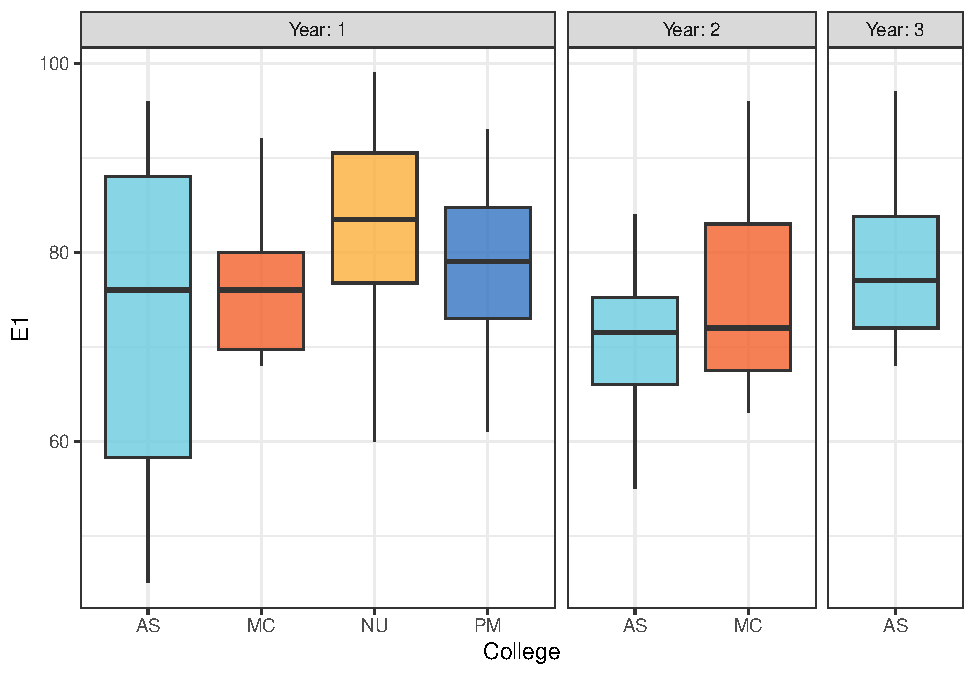
\includegraphics{_main_files/figure-latex/unnamed-chunk-44-1.pdf}

\begin{Shaded}
\begin{Highlighting}[]
\FunctionTok{ggplot}\NormalTok{(students, }\FunctionTok{aes}\NormalTok{(College, E1)) }\SpecialCharTok{+}
  \FunctionTok{geom\_boxplot}\NormalTok{(}\FunctionTok{aes}\NormalTok{(}\AttributeTok{fill =} \FunctionTok{stage}\NormalTok{(College, }\AttributeTok{after\_scale =} \FunctionTok{alpha}\NormalTok{(fill, }\FloatTok{0.8}\NormalTok{))), }\AttributeTok{show.legend =} \ConstantTok{FALSE}\NormalTok{) }\SpecialCharTok{+}
  \FunctionTok{facet\_grid}\NormalTok{(}\SpecialCharTok{\textasciitilde{}}\NormalTok{Year, }\AttributeTok{scales =} \StringTok{"free"}\NormalTok{, }\AttributeTok{space =} \StringTok{"free\_x"}\NormalTok{, }\AttributeTok{labeller =} \FunctionTok{labeller}\NormalTok{(}\AttributeTok{Year =}\NormalTok{ label\_both))}
\end{Highlighting}
\end{Shaded}

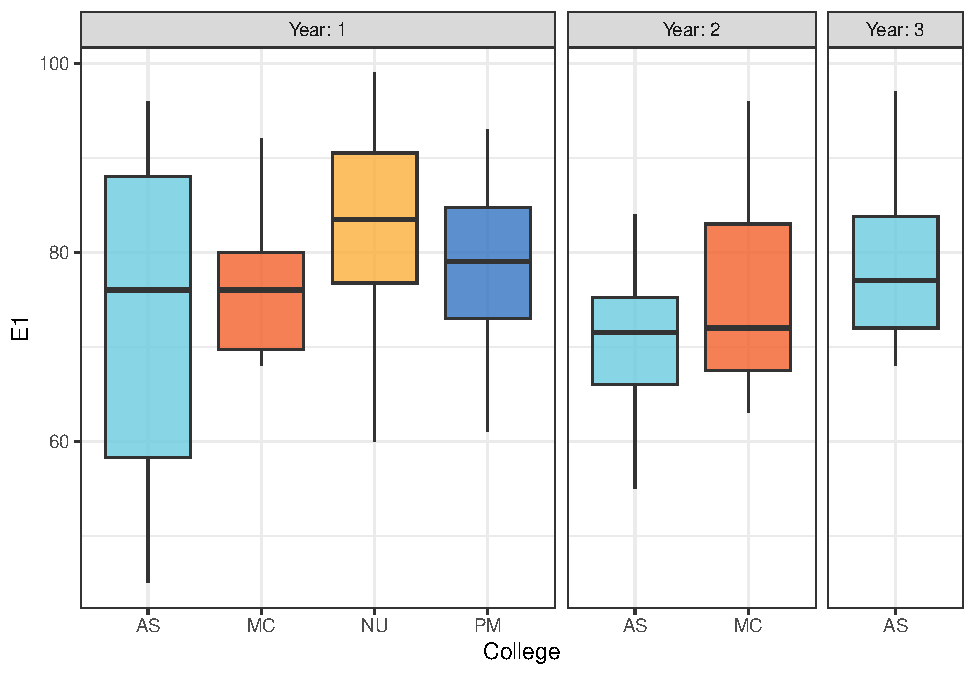
\includegraphics{_main_files/figure-latex/unnamed-chunk-44-2.pdf}

\begin{center}\rule{0.5\linewidth}{0.5pt}\end{center}

The coverage of the different methods below is divided into several sections:

\begin{enumerate}
\def\labelenumi{\arabic{enumi}.}
\tightlist
\item
  \protect\hyperlink{one-sample-t-test}{One-sample t-test}
\item
  \protect\hyperlink{other-hypothesis-tests}{Other Basic Hypothesis Tests}
\item
  \protect\hyperlink{one-way-anova}{One-way ANOVA and Multiple Comparisons}
\item
  \protect\hyperlink{regression-ancova}{Regression, Factorial ANOVA, and ANCOVA}
\item
  \protect\hyperlink{other-methods}{Other Methods}
\end{enumerate}

Each of them assumes you have created and attached the data frame \texttt{students} and created the objects \texttt{E1.1NU}, \texttt{E1.1AS}, \texttt{E3.1NU}, and \texttt{grp}.

\hypertarget{one-sample-t-test}{%
\section{One-sample t-test and interval}\label{one-sample-t-test}}

Test the null hypothesis that the mean score on \texttt{E1} for 1st year nursing students is greater than the historical exam average of 75.

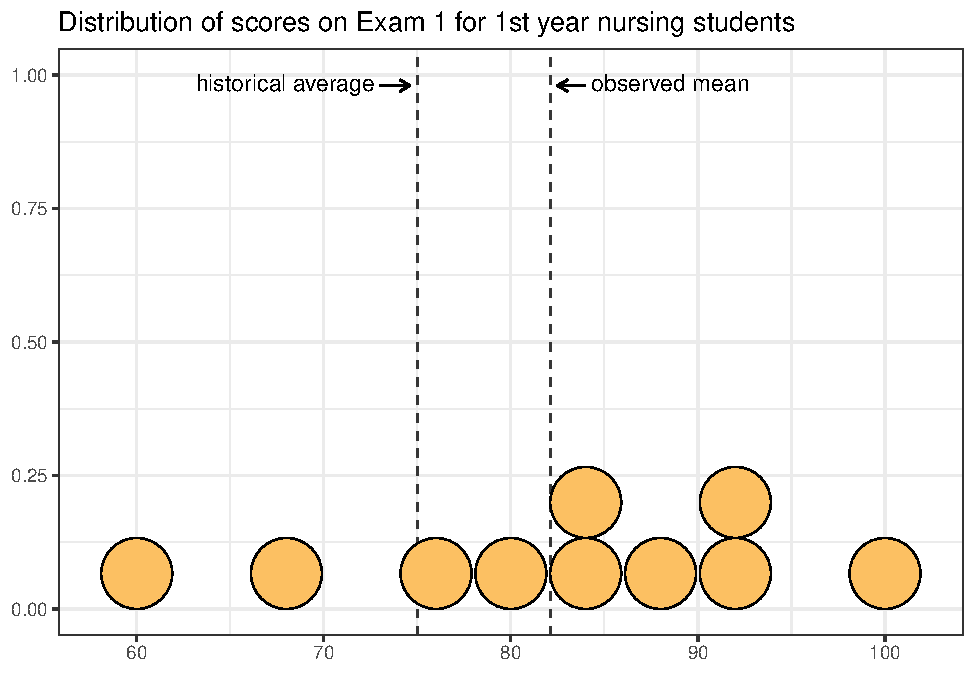
\includegraphics{_main_files/figure-latex/unnamed-chunk-45-1.pdf}

\begin{Shaded}
\begin{Highlighting}[]
\NormalTok{students }\SpecialCharTok{\%\textgreater{}\%} 
\NormalTok{  dplyr}\SpecialCharTok{::}\FunctionTok{filter}\NormalTok{(College }\SpecialCharTok{==} \StringTok{"NU"}\NormalTok{) }\SpecialCharTok{\%\textgreater{}\%} 
\NormalTok{  infer}\SpecialCharTok{::}\FunctionTok{t\_test}\NormalTok{(}\AttributeTok{response =}\NormalTok{ E1, }\AttributeTok{mu =} \DecValTok{75}\NormalTok{, }\AttributeTok{alternative =} \StringTok{"greater"}\NormalTok{) }\SpecialCharTok{\%\textgreater{}\%} 
\NormalTok{  pander}\SpecialCharTok{::}\FunctionTok{pander}\NormalTok{()}
\end{Highlighting}
\end{Shaded}

\begin{longtable}[]{@{}
  >{\centering\arraybackslash}p{(\columnwidth - 12\tabcolsep) * \real{0.1579}}
  >{\centering\arraybackslash}p{(\columnwidth - 12\tabcolsep) * \real{0.0921}}
  >{\centering\arraybackslash}p{(\columnwidth - 12\tabcolsep) * \real{0.1316}}
  >{\centering\arraybackslash}p{(\columnwidth - 12\tabcolsep) * \real{0.1842}}
  >{\centering\arraybackslash}p{(\columnwidth - 12\tabcolsep) * \real{0.1447}}
  >{\centering\arraybackslash}p{(\columnwidth - 12\tabcolsep) * \real{0.1447}}
  >{\centering\arraybackslash}p{(\columnwidth - 12\tabcolsep) * \real{0.1447}}@{}}
\toprule()
\begin{minipage}[b]{\linewidth}\centering
statistic
\end{minipage} & \begin{minipage}[b]{\linewidth}\centering
t\_df
\end{minipage} & \begin{minipage}[b]{\linewidth}\centering
p\_value
\end{minipage} & \begin{minipage}[b]{\linewidth}\centering
alternative
\end{minipage} & \begin{minipage}[b]{\linewidth}\centering
estimate
\end{minipage} & \begin{minipage}[b]{\linewidth}\centering
lower\_ci
\end{minipage} & \begin{minipage}[b]{\linewidth}\centering
upper\_ci
\end{minipage} \\
\midrule()
\endhead
1.906 & 9 & 0.04452 & greater & 82.1 & 75.27 & Inf \\
\bottomrule()
\end{longtable}

\textbf{Note} that this produces a one-sided confidence bound because of the alternative selected. To get the standard 95\% interval in the solutions, run it without the \texttt{alternative\ =\ "greater"} part (you don't need to specify \texttt{"two-sided"} because that is the default setting). The other option is \texttt{"less"}.

Using \texttt{help(t\_test)} we can also see that the default null hypothesis is \texttt{mu\ =\ 0}, the function can perform the two-sample tests, and \texttt{conf\_level} controls the confidence level for the confidence intervals.

In some cases it is useful to be able to retrieve only part of the output from a test. For example, a simulation study might only want to use the p-values. Because \texttt{infer::t\_test()} returns a data frame, the values can easily be extracted.

\begin{Shaded}
\begin{Highlighting}[]
\NormalTok{students }\SpecialCharTok{\%\textgreater{}\%} 
\NormalTok{  dplyr}\SpecialCharTok{::}\FunctionTok{filter}\NormalTok{(College }\SpecialCharTok{==} \StringTok{"NU"}\NormalTok{) }\SpecialCharTok{\%\textgreater{}\%} 
\NormalTok{  infer}\SpecialCharTok{::}\FunctionTok{t\_test}\NormalTok{(}\AttributeTok{response =}\NormalTok{ E1, }\AttributeTok{mu =} \DecValTok{75}\NormalTok{, }\AttributeTok{alternative =} \StringTok{"greater"}\NormalTok{) }\SpecialCharTok{\%\textgreater{}\%} 
  \FunctionTok{pull}\NormalTok{(p\_value)}
\end{Highlighting}
\end{Shaded}

\begin{verbatim}
## [1] 0.04451704
\end{verbatim}

If we save the output as an object, the values can be accessed using the \texttt{\$}. For example:

\begin{Shaded}
\begin{Highlighting}[]
\NormalTok{t.out }\OtherTok{\textless{}{-}}\NormalTok{ students }\SpecialCharTok{\%\textgreater{}\%} 
\NormalTok{  dplyr}\SpecialCharTok{::}\FunctionTok{filter}\NormalTok{(College }\SpecialCharTok{==} \StringTok{"NU"}\NormalTok{) }\SpecialCharTok{\%\textgreater{}\%} 
\NormalTok{  infer}\SpecialCharTok{::}\FunctionTok{t\_test}\NormalTok{(}\AttributeTok{response =}\NormalTok{ E1, }\AttributeTok{mu =} \DecValTok{75}\NormalTok{, }\AttributeTok{alternative =} \StringTok{"greater"}\NormalTok{) }

\NormalTok{t.out}\SpecialCharTok{$}\NormalTok{p\_value}
\end{Highlighting}
\end{Shaded}

\begin{verbatim}
## [1] 0.04451704
\end{verbatim}

\hypertarget{other-hypothesis-tests}{%
\section{Other Basic Hypothesis Tests}\label{other-hypothesis-tests}}

\hypertarget{two-sample-t-test-and-interval}{%
\subsection{Two-sample t-test and interval}\label{two-sample-t-test-and-interval}}

Test the null hypothesis that the mean on \texttt{E1} for 1st year students from arts and sciences is less than the mean for 1st year students from nursing.

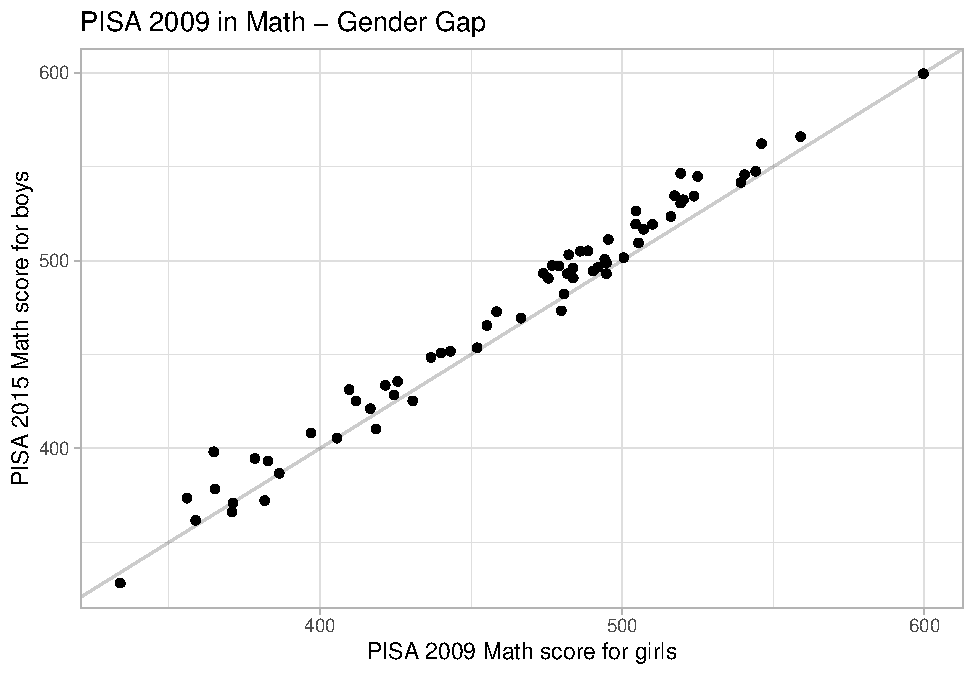
\includegraphics{_main_files/figure-latex/unnamed-chunk-50-1.pdf}

\begin{Shaded}
\begin{Highlighting}[]
\NormalTok{students }\SpecialCharTok{\%\textgreater{}\%}
\NormalTok{  dplyr}\SpecialCharTok{::}\FunctionTok{filter}\NormalTok{(College }\SpecialCharTok{\%in\%} \FunctionTok{c}\NormalTok{(}\StringTok{"NU"}\NormalTok{, }\StringTok{"AS"}\NormalTok{), Year }\SpecialCharTok{==} \DecValTok{1}\NormalTok{) }\SpecialCharTok{\%\textgreater{}\%}
\NormalTok{  infer}\SpecialCharTok{::}\FunctionTok{t\_test}\NormalTok{(}\AttributeTok{formula =}\NormalTok{ E1 }\SpecialCharTok{\textasciitilde{}}\NormalTok{ College, }
       \AttributeTok{order =} \FunctionTok{c}\NormalTok{(}\StringTok{"AS"}\NormalTok{, }\StringTok{"NU"}\NormalTok{),}
       \AttributeTok{alternative =} \StringTok{"less"}\NormalTok{, }
       \AttributeTok{var.equal =} \ConstantTok{TRUE}\NormalTok{) }\SpecialCharTok{\%\textgreater{}\%} 
\NormalTok{  pander}\SpecialCharTok{::}\FunctionTok{pander}\NormalTok{()}
\end{Highlighting}
\end{Shaded}

\begin{longtable}[]{@{}
  >{\centering\arraybackslash}p{(\columnwidth - 12\tabcolsep) * \real{0.1579}}
  >{\centering\arraybackslash}p{(\columnwidth - 12\tabcolsep) * \real{0.0921}}
  >{\centering\arraybackslash}p{(\columnwidth - 12\tabcolsep) * \real{0.1316}}
  >{\centering\arraybackslash}p{(\columnwidth - 12\tabcolsep) * \real{0.1842}}
  >{\centering\arraybackslash}p{(\columnwidth - 12\tabcolsep) * \real{0.1447}}
  >{\centering\arraybackslash}p{(\columnwidth - 12\tabcolsep) * \real{0.1447}}
  >{\centering\arraybackslash}p{(\columnwidth - 12\tabcolsep) * \real{0.1447}}@{}}
\toprule()
\begin{minipage}[b]{\linewidth}\centering
statistic
\end{minipage} & \begin{minipage}[b]{\linewidth}\centering
t\_df
\end{minipage} & \begin{minipage}[b]{\linewidth}\centering
p\_value
\end{minipage} & \begin{minipage}[b]{\linewidth}\centering
alternative
\end{minipage} & \begin{minipage}[b]{\linewidth}\centering
estimate
\end{minipage} & \begin{minipage}[b]{\linewidth}\centering
lower\_ci
\end{minipage} & \begin{minipage}[b]{\linewidth}\centering
upper\_ci
\end{minipage} \\
\midrule()
\endhead
-1.385 & 18 & 0.09152 & less & -9.6 & -Inf & 2.421 \\
\bottomrule()
\end{longtable}

\texttt{var.equal\ =\ TRUE} specifies use of the equal variances assumption. The default is variances not equal (or use \texttt{var.equal\ =\ FALSE}). Again, the confidence interval gotten using this code is the one-sided confidence bound. Use \texttt{two-sided} to get the confidence interval.

\hypertarget{paired-t-test-and-confidence-interval}{%
\subsection{Paired t-test and confidence interval}\label{paired-t-test-and-confidence-interval}}

Test that the mean for \texttt{E3} is greater than the mean of \texttt{E1} for first year nursing students.

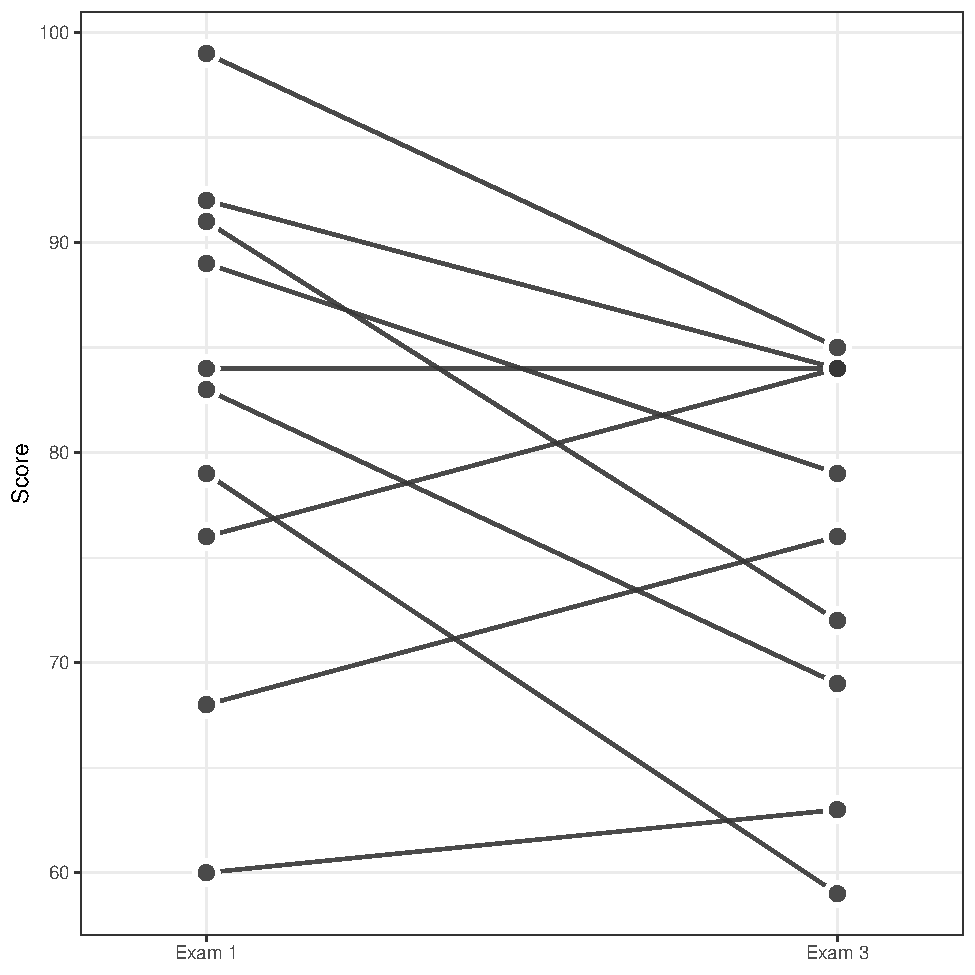
\includegraphics[width=0.8\linewidth]{_main_files/figure-latex/unnamed-chunk-53-1}

\begin{Shaded}
\begin{Highlighting}[]
\NormalTok{students }\SpecialCharTok{\%\textgreater{}\%} 
\NormalTok{  dplyr}\SpecialCharTok{::}\FunctionTok{filter}\NormalTok{(College }\SpecialCharTok{==} \StringTok{"NU"}\NormalTok{) }\SpecialCharTok{\%\textgreater{}\%} 
  \FunctionTok{mutate}\NormalTok{(}\AttributeTok{Change =}\NormalTok{ E3 }\SpecialCharTok{{-}}\NormalTok{ E1) }\SpecialCharTok{\%\textgreater{}\%} 
\NormalTok{  infer}\SpecialCharTok{::}\FunctionTok{t\_test}\NormalTok{(}\AttributeTok{response =}\NormalTok{ Change, }\AttributeTok{alternative =} \StringTok{"greater"}\NormalTok{) }\SpecialCharTok{\%\textgreater{}\%} 
\NormalTok{  pander}\SpecialCharTok{::}\FunctionTok{pander}\NormalTok{()}
\end{Highlighting}
\end{Shaded}

\begin{longtable}[]{@{}
  >{\centering\arraybackslash}p{(\columnwidth - 12\tabcolsep) * \real{0.1579}}
  >{\centering\arraybackslash}p{(\columnwidth - 12\tabcolsep) * \real{0.0921}}
  >{\centering\arraybackslash}p{(\columnwidth - 12\tabcolsep) * \real{0.1316}}
  >{\centering\arraybackslash}p{(\columnwidth - 12\tabcolsep) * \real{0.1842}}
  >{\centering\arraybackslash}p{(\columnwidth - 12\tabcolsep) * \real{0.1447}}
  >{\centering\arraybackslash}p{(\columnwidth - 12\tabcolsep) * \real{0.1447}}
  >{\centering\arraybackslash}p{(\columnwidth - 12\tabcolsep) * \real{0.1447}}@{}}
\toprule()
\begin{minipage}[b]{\linewidth}\centering
statistic
\end{minipage} & \begin{minipage}[b]{\linewidth}\centering
t\_df
\end{minipage} & \begin{minipage}[b]{\linewidth}\centering
p\_value
\end{minipage} & \begin{minipage}[b]{\linewidth}\centering
alternative
\end{minipage} & \begin{minipage}[b]{\linewidth}\centering
estimate
\end{minipage} & \begin{minipage}[b]{\linewidth}\centering
lower\_ci
\end{minipage} & \begin{minipage}[b]{\linewidth}\centering
upper\_ci
\end{minipage} \\
\midrule()
\endhead
-1.962 & 9 & 0.9593 & greater & -6.6 & -12.77 & Inf \\
\bottomrule()
\end{longtable}

Another option for conducting a paired t-test is to use the \texttt{t.test()} function with \texttt{paired\ =\ T}. The output, of course, is the same as conducting the one-sample t test on the differences.

\begin{Shaded}
\begin{Highlighting}[]
\DocumentationTok{\#\# The correct paired test}
\FunctionTok{t.test}\NormalTok{(E3}\FloatTok{.1}\NormalTok{NU, E1}\FloatTok{.1}\NormalTok{NU, }\AttributeTok{alternative =} \StringTok{"greater"}\NormalTok{, }\AttributeTok{paired =}\NormalTok{ T)}
\end{Highlighting}
\end{Shaded}

\begin{verbatim}
## 
##  Paired t-test
## 
## data:  E3.1NU and E1.1NU
## t = -1.962, df = 9, p-value = 0.9593
## alternative hypothesis: true mean difference is greater than 0
## 95 percent confidence interval:
##  -12.76634       Inf
## sample estimates:
## mean difference 
##            -6.6
\end{verbatim}

\hypertarget{chi-square-test-and-interval-for-one-variance}{%
\subsection{Chi-square test and interval for one variance}\label{chi-square-test-and-interval-for-one-variance}}

Test whether the standard deviation of \texttt{E1} is greater than 10 for the first year nursing students.

R doesn't have this test built in (which isn't that horrible since we should probably never do it\ldots{} but it does make it odd that they have the F-test for two variances then.) In any case its pretty easy to write a function to do it. To analyze the data, cut and paste the function in, and then run it on your data. Or, it can be read in using \texttt{source("code/TWRfns.txt")}.

\begin{Shaded}
\begin{Highlighting}[]
\NormalTok{chisquare.var }\OtherTok{\textless{}{-}} \ControlFlowTok{function}\NormalTok{(y, }\AttributeTok{sigma2 =} \DecValTok{1}\NormalTok{, }\AttributeTok{alpha =} \FloatTok{0.05}\NormalTok{) \{}
\NormalTok{  n }\OtherTok{\textless{}{-}} \FunctionTok{length}\NormalTok{(y)}
\NormalTok{  chisquare }\OtherTok{\textless{}{-}}\NormalTok{ (n }\SpecialCharTok{{-}} \DecValTok{1}\NormalTok{) }\SpecialCharTok{*} \FunctionTok{var}\NormalTok{(y) }\SpecialCharTok{/}\NormalTok{ sigma2}
\NormalTok{  pval.low }\OtherTok{\textless{}{-}} \FunctionTok{pchisq}\NormalTok{(chisquare, }\AttributeTok{df =}\NormalTok{ n }\SpecialCharTok{{-}} \DecValTok{1}\NormalTok{)}
\NormalTok{  pval.hi }\OtherTok{\textless{}{-}} \DecValTok{1} \SpecialCharTok{{-}} \FunctionTok{pchisq}\NormalTok{(chisquare, }\AttributeTok{df =}\NormalTok{ n }\SpecialCharTok{{-}} \DecValTok{1}\NormalTok{)}
\NormalTok{  pval.not }\OtherTok{\textless{}{-}} \DecValTok{2} \SpecialCharTok{*} \FunctionTok{min}\NormalTok{(pval.low, pval.hi)}
\NormalTok{  cilow }\OtherTok{\textless{}{-}}\NormalTok{ (n }\SpecialCharTok{{-}} \DecValTok{1}\NormalTok{) }\SpecialCharTok{*} \FunctionTok{var}\NormalTok{(y) }\SpecialCharTok{/} \FunctionTok{qchisq}\NormalTok{(}\DecValTok{1} \SpecialCharTok{{-}}\NormalTok{ alpha }\SpecialCharTok{/} \DecValTok{2}\NormalTok{, }\AttributeTok{df =}\NormalTok{ n }\SpecialCharTok{{-}} \DecValTok{1}\NormalTok{)}
\NormalTok{  cihi }\OtherTok{\textless{}{-}}\NormalTok{ (n }\SpecialCharTok{{-}} \DecValTok{1}\NormalTok{) }\SpecialCharTok{*} \FunctionTok{var}\NormalTok{(y) }\SpecialCharTok{/} \FunctionTok{qchisq}\NormalTok{(alpha }\SpecialCharTok{/} \DecValTok{2}\NormalTok{, }\AttributeTok{df =}\NormalTok{ n }\SpecialCharTok{{-}} \DecValTok{1}\NormalTok{)}
  \FunctionTok{list}\NormalTok{(}
    \AttributeTok{chisquare =}\NormalTok{ chisquare, }\AttributeTok{pval.for.less.than =}\NormalTok{ pval.low,}
    \AttributeTok{pval.for.greater.than =}\NormalTok{ pval.hi, }\AttributeTok{pval.for.not.equal =}\NormalTok{ pval.not,}
    \AttributeTok{ci.for.variance =} \FunctionTok{c}\NormalTok{(cilow, cihi), }\AttributeTok{ci.for.sd =} \FunctionTok{c}\NormalTok{(}\FunctionTok{sqrt}\NormalTok{(cilow), }\FunctionTok{sqrt}\NormalTok{(cihi))}
\NormalTok{  )}
\NormalTok{\}}
\end{Highlighting}
\end{Shaded}

\begin{Shaded}
\begin{Highlighting}[]
\FunctionTok{chisquare.var}\NormalTok{(E1}\FloatTok{.1}\NormalTok{NU, }\AttributeTok{sigma2 =} \DecValTok{10}\SpecialCharTok{\^{}}\DecValTok{2}\NormalTok{)}
\end{Highlighting}
\end{Shaded}

\begin{verbatim}
## $chisquare
## [1] 12.489
## 
## $pval.for.less.than
## [1] 0.8128762
## 
## $pval.for.greater.than
## [1] 0.1871238
## 
## $pval.for.not.equal
## [1] 0.3742476
## 
## $ci.for.variance
## [1]  65.65291 462.48884
## 
## $ci.for.sd
## [1]  8.102648 21.505554
\end{verbatim}

Note that the confidence intervals here are sub-optimal in terms of length because they place an equal amount of area in each end.

\hypertarget{f-test-for-two-variances}{%
\subsection{F test for two variances}\label{f-test-for-two-variances}}

Test whether the variance of \texttt{E1} for the first year nursing students is equal to the variance of \texttt{E1} for the first year arts and sciences students.

\begin{Shaded}
\begin{Highlighting}[]
\FunctionTok{var.test}\NormalTok{(E1}\FloatTok{.1}\NormalTok{NU, E1}\FloatTok{.1}\NormalTok{AS)}
\end{Highlighting}
\end{Shaded}

\begin{verbatim}
## 
##  F test to compare two variances
## 
## data:  E1.1NU and E1.1AS
## F = 0.40595, num df = 9, denom df = 9, p-value = 0.1954
## alternative hypothesis: true ratio of variances is not equal to 1
## 95 percent confidence interval:
##  0.1008318 1.6343456
## sample estimates:
## ratio of variances 
##          0.4059483
\end{verbatim}

\hypertarget{two-sample-modified-levenes-test}{%
\subsection{Two-sample Modified Levene's Test}\label{two-sample-modified-levenes-test}}

Test of whether the variance of E1 for the first year nursing students is equal to the variance of E1 for the first year arts and sciences students.

R doesn't contain a built in function for the Modified Levene's test, but it can be carried out simply by running the two sample t.test on the right values.

\begin{Shaded}
\begin{Highlighting}[]
\FunctionTok{t.test}\NormalTok{(}\FunctionTok{abs}\NormalTok{(E1}\FloatTok{.1}\NormalTok{NU }\SpecialCharTok{{-}} \FunctionTok{median}\NormalTok{(E1}\FloatTok{.1}\NormalTok{NU)), }\FunctionTok{abs}\NormalTok{(E1}\FloatTok{.1}\NormalTok{AS }\SpecialCharTok{{-}} \FunctionTok{median}\NormalTok{(E1}\FloatTok{.1}\NormalTok{AS)), }\AttributeTok{var.equal =}\NormalTok{ T)}
\end{Highlighting}
\end{Shaded}

\begin{verbatim}
## 
##  Two Sample t-test
## 
## data:  abs(E1.1NU - median(E1.1NU)) and abs(E1.1AS - median(E1.1AS))
## t = -1.3395, df = 18, p-value = 0.1971
## alternative hypothesis: true difference in means is not equal to 0
## 95 percent confidence interval:
##  -14.382926   3.182926
## sample estimates:
## mean of x mean of y 
##       8.9      14.5
\end{verbatim}

Of course the means this is testing about are the means of the absolute deviation from the median. If that measure of spread is different between the two populations, then the variances should be different as well.

The packages \textbf{car} and \textbf{lawstat} have built in modified Levene's test functions, but they require having a response variable and a group variable (like in ANOVA). An easy function for the two sample case would be:

\begin{Shaded}
\begin{Highlighting}[]
\NormalTok{levene2 }\OtherTok{\textless{}{-}} \ControlFlowTok{function}\NormalTok{(data1, data2) \{}
  \FunctionTok{print}\NormalTok{(}\StringTok{"p{-}value for testing null hypothesis of equal variances"}\NormalTok{)}
  \FunctionTok{t.test}\NormalTok{(}\FunctionTok{abs}\NormalTok{(data1 }\SpecialCharTok{{-}} \FunctionTok{median}\NormalTok{(data1)), }\FunctionTok{abs}\NormalTok{(data2 }\SpecialCharTok{{-}} \FunctionTok{median}\NormalTok{(data2)), }\AttributeTok{var.equal =}\NormalTok{ T)}\SpecialCharTok{$}\NormalTok{p.value}
\NormalTok{\}}

\FunctionTok{levene2}\NormalTok{(E1}\FloatTok{.1}\NormalTok{NU, E1}\FloatTok{.1}\NormalTok{AS)}
\end{Highlighting}
\end{Shaded}

\begin{verbatim}
## [1] "p-value for testing null hypothesis of equal variances"
\end{verbatim}

\begin{verbatim}
## [1] 0.1970608
\end{verbatim}

\hypertarget{one-way-anova}{%
\section{One-way ANOVA and Multiple Comparisons}\label{one-way-anova}}

\hypertarget{one-way-anova-1}{%
\subsection{One-way ANOVA}\label{one-way-anova-1}}

Test whether the means of E1 are equal for the seven populations of students.

The basic function for conducting an ANOVA (or any linear model) is \texttt{lm()}:

\begin{Shaded}
\begin{Highlighting}[]
\FunctionTok{lm}\NormalTok{(E1 }\SpecialCharTok{\textasciitilde{}}\NormalTok{ grp)}
\end{Highlighting}
\end{Shaded}

\begin{verbatim}
## 
## Call:
## lm(formula = E1 ~ grp)
## 
## Coefficients:
## (Intercept)       grp1MC       grp1NU       grp1PM       grp2AS       grp2MC  
##        72.5          3.8          9.6          5.6         -1.8          3.3  
##      grp3AS  
##         6.6
\end{verbatim}

The \texttt{\textasciitilde{}} indicates that you are specifying a model equation. The variable to the left of the tilde is the response variable, and the variable to the right is the predictor variable. (In multiple regression and more complicated ANOVA there can be multiple predictor variables).

Unfortunately the output from \texttt{lm()} seems pretty meager - it is just the estimates of the parameters in the model equation. Using:

\begin{Shaded}
\begin{Highlighting}[]
\FunctionTok{attributes}\NormalTok{(}\FunctionTok{lm}\NormalTok{(E1 }\SpecialCharTok{\textasciitilde{}}\NormalTok{ grp))}
\end{Highlighting}
\end{Shaded}

\begin{verbatim}
## $names
##  [1] "coefficients"  "residuals"     "effects"       "rank"         
##  [5] "fitted.values" "assign"        "qr"            "df.residual"  
##  [9] "contrasts"     "xlevels"       "call"          "terms"        
## [13] "model"        
## 
## $class
## [1] "lm"
\end{verbatim}

shows that there is a lot more behind the scenes. The functions \texttt{anova()}, \texttt{summary()}, and \texttt{plot()} can be used to extract much of this information.

\begin{Shaded}
\begin{Highlighting}[]
\NormalTok{E1fit }\OtherTok{\textless{}{-}} \FunctionTok{lm}\NormalTok{(E1 }\SpecialCharTok{\textasciitilde{}}\NormalTok{ grp)}
\FunctionTok{anova}\NormalTok{(E1fit)}
\end{Highlighting}
\end{Shaded}

\begin{verbatim}
## Analysis of Variance Table
## 
## Response: E1
##           Df Sum Sq Mean Sq F value Pr(>F)
## grp        6  907.3  151.22  1.1563  0.341
## Residuals 63 8239.0  130.78
\end{verbatim}

\begin{Shaded}
\begin{Highlighting}[]
\FunctionTok{summary}\NormalTok{(E1fit)}
\end{Highlighting}
\end{Shaded}

\begin{verbatim}
## 
## Call:
## lm(formula = E1 ~ grp)
## 
## Residuals:
##    Min     1Q Median     3Q    Max 
## -27.50  -6.80   0.10   6.45  23.50 
## 
## Coefficients:
##             Estimate Std. Error t value Pr(>|t|)    
## (Intercept)   72.500      3.616  20.048   <2e-16 ***
## grp1MC         3.800      5.114   0.743   0.4602    
## grp1NU         9.600      5.114   1.877   0.0651 .  
## grp1PM         5.600      5.114   1.095   0.2777    
## grp2AS        -1.800      5.114  -0.352   0.7260    
## grp2MC         3.300      5.114   0.645   0.5211    
## grp3AS         6.600      5.114   1.291   0.2016    
## ---
## Signif. codes:  0 '***' 0.001 '**' 0.01 '*' 0.05 '.' 0.1 ' ' 1
## 
## Residual standard error: 11.44 on 63 degrees of freedom
## Multiple R-squared:  0.0992, Adjusted R-squared:  0.01341 
## F-statistic: 1.156 on 6 and 63 DF,  p-value: 0.341
\end{verbatim}

\begin{Shaded}
\begin{Highlighting}[]
\FunctionTok{par}\NormalTok{(}\AttributeTok{mfrow =} \FunctionTok{c}\NormalTok{(}\DecValTok{1}\NormalTok{, }\DecValTok{2}\NormalTok{))}
\FunctionTok{plot}\NormalTok{(E1fit, }\DecValTok{1}\NormalTok{)}
\FunctionTok{plot}\NormalTok{(E1fit, }\DecValTok{2}\NormalTok{)}
\end{Highlighting}
\end{Shaded}

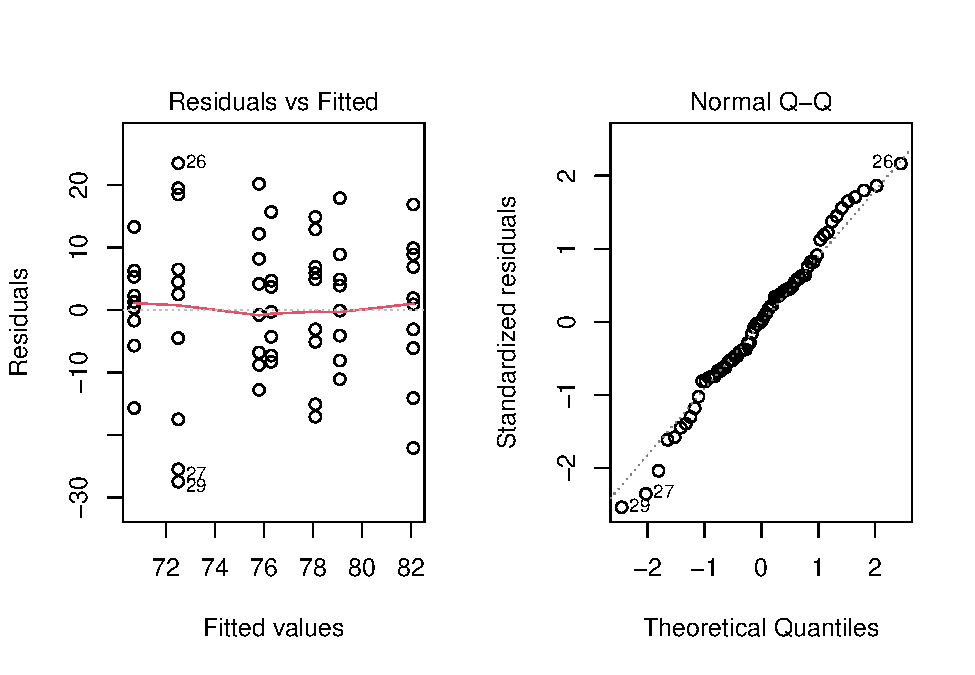
\includegraphics{_main_files/figure-latex/unnamed-chunk-66-1.pdf}

\begin{Shaded}
\begin{Highlighting}[]
\FunctionTok{par}\NormalTok{(}\AttributeTok{mfrow =} \FunctionTok{c}\NormalTok{(}\DecValTok{1}\NormalTok{, }\DecValTok{1}\NormalTok{))}
\end{Highlighting}
\end{Shaded}

The 1 and 2 in the plot function request the first two graphs that are automatically produced when plotting the result of \texttt{lm()} - the first is the residual vs.~predicted plot, and the second is the qq-plot of the residuals. Leaving out the number will produce four plots, but only one at a time (you have to click on the graphics window to advance to the next one).

In some cases it is necessary to enter the data on your own, and then it is important to be sure that the group variable is a ``factor''. For example, imagine that you had the vector E1 entered, but did not have the vector of group memberships yet. We know however that the test scores go with different groups in sets of 10 (observations 1-10 are \texttt{1NU}, 11-20 are \texttt{1PM}, etc\ldots). One way we could do a set of labels is:

\begin{Shaded}
\begin{Highlighting}[]
\NormalTok{grplabs }\OtherTok{\textless{}{-}} \FunctionTok{c}\NormalTok{(}
  \FunctionTok{rep}\NormalTok{(}\DecValTok{1}\NormalTok{, }\DecValTok{10}\NormalTok{), }\FunctionTok{rep}\NormalTok{(}\DecValTok{2}\NormalTok{, }\DecValTok{10}\NormalTok{), }\FunctionTok{rep}\NormalTok{(}\DecValTok{3}\NormalTok{, }\DecValTok{10}\NormalTok{),}
  \FunctionTok{rep}\NormalTok{(}\DecValTok{4}\NormalTok{, }\DecValTok{10}\NormalTok{), }\FunctionTok{rep}\NormalTok{(}\DecValTok{5}\NormalTok{, }\DecValTok{10}\NormalTok{), }\FunctionTok{rep}\NormalTok{(}\DecValTok{6}\NormalTok{, }\DecValTok{10}\NormalTok{), }\FunctionTok{rep}\NormalTok{(}\DecValTok{7}\NormalTok{, }\DecValTok{10}\NormalTok{)}
\NormalTok{)}
\NormalTok{grplabs}
\end{Highlighting}
\end{Shaded}

\begin{verbatim}
##  [1] 1 1 1 1 1 1 1 1 1 1 2 2 2 2 2 2 2 2 2 2 3 3 3 3 3 3 3 3 3 3 4 4 4 4 4 4 4 4
## [39] 4 4 5 5 5 5 5 5 5 5 5 5 6 6 6 6 6 6 6 6 6 6 7 7 7 7 7 7 7 7 7 7
\end{verbatim}

The rep repeats the value in the first spot the number of times indicated in the second. Trying

\begin{Shaded}
\begin{Highlighting}[]
\FunctionTok{lm}\NormalTok{(E1 }\SpecialCharTok{\textasciitilde{}}\NormalTok{ grplabs)}
\end{Highlighting}
\end{Shaded}

\begin{verbatim}
## 
## Call:
## lm(formula = E1 ~ grplabs)
## 
## Coefficients:
## (Intercept)      grplabs  
##     78.6429      -0.5679
\end{verbatim}

gives a very different result from before though. Because the predictor variable is numeric, by default it attempted to do a regression instead of an ANOVA. Using:

\begin{Shaded}
\begin{Highlighting}[]
\NormalTok{grplabs }\OtherTok{\textless{}{-}} \FunctionTok{as.factor}\NormalTok{(grplabs)}
\FunctionTok{lm}\NormalTok{(E1 }\SpecialCharTok{\textasciitilde{}}\NormalTok{ grplabs)}
\end{Highlighting}
\end{Shaded}

\begin{verbatim}
## 
## Call:
## lm(formula = E1 ~ grplabs)
## 
## Coefficients:
## (Intercept)     grplabs2     grplabs3     grplabs4     grplabs5     grplabs6  
##        82.1         -4.0         -9.6        -11.4         -3.0         -5.8  
##    grplabs7  
##        -6.3
\end{verbatim}

solves that problem. If we had entered the names of the various groups in quotation marks, instead of 1-7, then the grplabs would have been characters instead of numeric, and it would have worked without being factors (although some other functions might give a warning message).

\hypertarget{modified-levene-test}{%
\subsection{Modified Levene Test}\label{modified-levene-test}}

Test whether the variances of E2 are equal for the seven populations of students.

The modified Levene test is available in the package car, so if that package has been downloaded it could be conducted using.

\begin{Shaded}
\begin{Highlighting}[]
\FunctionTok{library}\NormalTok{(car)}
\FunctionTok{leveneTest}\NormalTok{(E1, grp)}
\end{Highlighting}
\end{Shaded}

\begin{verbatim}
## Levene's Test for Homogeneity of Variance (center = median)
##       Df F value  Pr(>F)  
## group  6  1.9679 0.08363 .
##       63                  
## ---
## Signif. codes:  0 '***' 0.001 '**' 0.01 '*' 0.05 '.' 0.1 ' ' 1
\end{verbatim}

\hypertarget{all-pairwise-comparisons---tukeys-hsd-and-scheffe}{%
\subsection{All Pairwise Comparisons - Tukey's HSD and Scheffe}\label{all-pairwise-comparisons---tukeys-hsd-and-scheffe}}

Simultaneously construct confidence intervals around the differences in the mean of E2 between each pair of groups, or test the hypotheses of equality of the mean E2 score between each pair of groups.

R has a built in function TukeyHSD that will construct the intervals in the balanced case, and includes an adjustment for the slightly unbalanced cases.

\begin{Shaded}
\begin{Highlighting}[]
\FunctionTok{TukeyHSD}\NormalTok{(}\FunctionTok{aov}\NormalTok{(E2 }\SpecialCharTok{\textasciitilde{}}\NormalTok{ grp))}
\end{Highlighting}
\end{Shaded}

\begin{verbatim}
##   Tukey multiple comparisons of means
##     95% family-wise confidence level
## 
## Fit: aov(formula = E2 ~ grp)
## 
## $grp
##          diff         lwr       upr     p adj
## 1MC-1AS  16.7  -3.8321876 37.232188 0.1853530
## 1NU-1AS  23.2   2.6678124 43.732188 0.0169654
## 1PM-1AS   6.5 -14.0321876 27.032188 0.9597899
## 2AS-1AS   0.8 -19.7321876 21.332188 0.9999997
## 2MC-1AS  19.8  -0.7321876 40.332188 0.0657667
## 3AS-1AS  14.9  -5.6321876 35.432188 0.3049582
## 1NU-1MC   6.5 -14.0321876 27.032188 0.9597899
## 1PM-1MC -10.2 -30.7321876 10.332188 0.7360677
## 2AS-1MC -15.9 -36.4321876  4.632188 0.2336176
## 2MC-1MC   3.1 -17.4321876 23.632188 0.9992362
## 3AS-1MC  -1.8 -22.3321876 18.732188 0.9999677
## 1PM-1NU -16.7 -37.2321876  3.832188 0.1853530
## 2AS-1NU -22.4 -42.9321876 -1.867812 0.0237608
## 2MC-1NU  -3.4 -23.9321876 17.132188 0.9987091
## 3AS-1NU  -8.3 -28.8321876 12.232188 0.8792779
## 2AS-1PM  -5.7 -26.2321876 14.832188 0.9789714
## 2MC-1PM  13.3  -7.2321876 33.832188 0.4417963
## 3AS-1PM   8.4 -12.1321876 28.932188 0.8731517
## 2MC-2AS  19.0  -1.5321876 39.532188 0.0876541
## 3AS-2AS  14.1  -6.4321876 34.632188 0.3702996
## 3AS-2MC  -4.9 -25.4321876 15.632188 0.9903950
\end{verbatim}

The structure is a little inelegant (it uses aov, an alternate to anova on the original lm statement). The output is also not in the prettiest form\ldots{} although that might be the only form that works if it is unbalanced.

As an alternative the function allpairs below will make the ``prettier'' display for either Tukey's HSD or Scheffe's method in the case where the different groups/treatments all have the same sample size. To run it, simply copy in the function as is, and then run it with the appropriate data.

\begin{Shaded}
\begin{Highlighting}[]
\DocumentationTok{\#\# The following function performs all pairwise comparisons using either Tukey\textquotesingle{}s HSD ("Tukey") or Scheffe\textquotesingle{}s method ("Scheffe").}
\DocumentationTok{\#\# The function only needs to be copied in once.}
\DocumentationTok{\#\# }\AlertTok{NOTE}\DocumentationTok{:  This function requires that all treatments have \#  equal sample size.}

\NormalTok{allpairs }\OtherTok{\textless{}{-}} \ControlFlowTok{function}\NormalTok{(y, treat, }\AttributeTok{method =} \StringTok{"Tukey"}\NormalTok{, }\AttributeTok{alpha =} \FloatTok{0.05}\NormalTok{) \{}
\NormalTok{  dat.reord }\OtherTok{\textless{}{-}} \FunctionTok{order}\NormalTok{(treat)}
\NormalTok{  treat }\OtherTok{\textless{}{-}}\NormalTok{ treat[dat.reord]}
\NormalTok{  y }\OtherTok{\textless{}{-}}\NormalTok{ y[dat.reord]}
\NormalTok{  s2w }\OtherTok{\textless{}{-}} \FunctionTok{anova}\NormalTok{(}\FunctionTok{lm}\NormalTok{(y }\SpecialCharTok{\textasciitilde{}}\NormalTok{ treat))[}\DecValTok{2}\NormalTok{, }\DecValTok{3}\NormalTok{]}
\NormalTok{  t }\OtherTok{\textless{}{-}} \FunctionTok{length}\NormalTok{(}\FunctionTok{table}\NormalTok{(treat))}
\NormalTok{  n }\OtherTok{\textless{}{-}} \FunctionTok{length}\NormalTok{(y) }\SpecialCharTok{/}\NormalTok{ t}
\NormalTok{  df }\OtherTok{\textless{}{-}}\NormalTok{ n }\SpecialCharTok{*}\NormalTok{ t }\SpecialCharTok{{-}}\NormalTok{ t}
\NormalTok{  qval }\OtherTok{\textless{}{-}} \FunctionTok{qtukey}\NormalTok{(}\DecValTok{1} \SpecialCharTok{{-}}\NormalTok{ alpha, t, df)}
  \ControlFlowTok{if}\NormalTok{ (method }\SpecialCharTok{==} \StringTok{"Tukey"}\NormalTok{) \{}
\NormalTok{    stat }\OtherTok{\textless{}{-}}\NormalTok{ qval }\SpecialCharTok{*} \FunctionTok{sqrt}\NormalTok{(s2w }\SpecialCharTok{/}\NormalTok{ n)}
\NormalTok{  \}}
  \ControlFlowTok{if}\NormalTok{ (method }\SpecialCharTok{==} \StringTok{"Scheffe"}\NormalTok{) \{}
\NormalTok{    stat }\OtherTok{\textless{}{-}}
      \FunctionTok{sqrt}\NormalTok{(}\DecValTok{2} \SpecialCharTok{*}\NormalTok{ s2w }\SpecialCharTok{/}\NormalTok{ n }\SpecialCharTok{*}\NormalTok{ (t }\SpecialCharTok{{-}} \DecValTok{1}\NormalTok{) }\SpecialCharTok{*} \FunctionTok{qf}\NormalTok{(}\DecValTok{1} \SpecialCharTok{{-}}\NormalTok{ alpha, t }\SpecialCharTok{{-}} \DecValTok{1}\NormalTok{, df))}
\NormalTok{  \}}
\NormalTok{  chars }\OtherTok{\textless{}{-}} \FunctionTok{c}\NormalTok{(}
    \StringTok{"A "}\NormalTok{, }\StringTok{"B "}\NormalTok{, }\StringTok{"C "}\NormalTok{, }\StringTok{"D "}\NormalTok{, }\StringTok{"E "}\NormalTok{, }\StringTok{"F "}\NormalTok{, }\StringTok{"G "}\NormalTok{, }\StringTok{"H "}\NormalTok{,}
    \StringTok{"I "}\NormalTok{, }\StringTok{"J "}\NormalTok{, }\StringTok{"L "}\NormalTok{, }\StringTok{"M "}\NormalTok{, }\StringTok{"N "}\NormalTok{, }\StringTok{"O "}\NormalTok{, }\StringTok{"P "}\NormalTok{, }\StringTok{"Q "}
\NormalTok{  )}
\NormalTok{  means }\OtherTok{\textless{}{-}} \FunctionTok{tapply}\NormalTok{(y, treat, mean)}
\NormalTok{  ord.means }\OtherTok{\textless{}{-}} \FunctionTok{order}\NormalTok{(}\SpecialCharTok{{-}}\NormalTok{means)}
\NormalTok{  treat }\OtherTok{\textless{}{-}}\NormalTok{ treat[ord.means]}
\NormalTok{  means }\OtherTok{\textless{}{-}}\NormalTok{ means[ord.means]}
\NormalTok{  grp }\OtherTok{\textless{}{-}} \DecValTok{1}
\NormalTok{  current }\OtherTok{\textless{}{-}} \DecValTok{1}
\NormalTok{  last }\OtherTok{\textless{}{-}} \DecValTok{0}
\NormalTok{  lastsofar }\OtherTok{\textless{}{-}} \DecValTok{0}
\NormalTok{  charmat }\OtherTok{\textless{}{-}} \ConstantTok{NULL}
  \ControlFlowTok{while}\NormalTok{ (last }\SpecialCharTok{\textless{}}\NormalTok{ t) \{}
\NormalTok{    newchar }\OtherTok{\textless{}{-}} \FunctionTok{rep}\NormalTok{(}\StringTok{"  "}\NormalTok{, t)}
    \ControlFlowTok{for}\NormalTok{ (i }\ControlFlowTok{in}\NormalTok{ current}\SpecialCharTok{:}\NormalTok{t) \{}
      \ControlFlowTok{if}\NormalTok{ (}\FunctionTok{abs}\NormalTok{(means[current] }\SpecialCharTok{{-}}\NormalTok{ means[i]) }\SpecialCharTok{\textless{}}\NormalTok{ stat) \{}
\NormalTok{        newchar[i] }\OtherTok{\textless{}{-}}\NormalTok{ chars[grp]}
\NormalTok{        last }\OtherTok{\textless{}{-}}\NormalTok{ i}
\NormalTok{      \}}
\NormalTok{    \}}
\NormalTok{    current }\OtherTok{\textless{}{-}}\NormalTok{ current }\SpecialCharTok{+} \DecValTok{1}
    \ControlFlowTok{if}\NormalTok{ (last }\SpecialCharTok{\textgreater{}}\NormalTok{ lastsofar) \{}
\NormalTok{      charmat }\OtherTok{\textless{}{-}} \FunctionTok{cbind}\NormalTok{(charmat, newchar)}
\NormalTok{      grp }\OtherTok{\textless{}{-}}\NormalTok{ grp }\SpecialCharTok{+} \DecValTok{1}
\NormalTok{      lastsofar }\OtherTok{\textless{}{-}}\NormalTok{ last}
\NormalTok{    \}}
\NormalTok{  \}}
\NormalTok{  charmat }\OtherTok{\textless{}{-}} \FunctionTok{apply}\NormalTok{(charmat, }\DecValTok{1}\NormalTok{, }\StringTok{"paste"}\NormalTok{, }\AttributeTok{sep =} \StringTok{""}\NormalTok{, }\AttributeTok{collapse =} \StringTok{""}\NormalTok{)}
  \FunctionTok{list}\NormalTok{(}
    \AttributeTok{Method =} \FunctionTok{paste}\NormalTok{(method, }\StringTok{", alpha="}\NormalTok{, }\FunctionTok{as.character}\NormalTok{(alpha),}
      \AttributeTok{sep =} \StringTok{""}\NormalTok{, }\AttributeTok{collapse =} \StringTok{""}
\NormalTok{    ),}
    \AttributeTok{Critical.Val =}\NormalTok{ stat,}
    \AttributeTok{Display =} \FunctionTok{data.frame}\NormalTok{(}\AttributeTok{Grp =}\NormalTok{ charmat, }\AttributeTok{Mean =}\NormalTok{ means)}
\NormalTok{  )}
\NormalTok{\}}


\FunctionTok{allpairs}\NormalTok{(E2, grp)}
\end{Highlighting}
\end{Shaded}

\begin{verbatim}
## $Method
## [1] "Tukey, alpha=0.05"
## 
## $Critical.Val
## [1] 20.53219
## 
## $Display
##      Grp Mean
## 1NU A    81.9
## 2MC A B  78.5
## 1MC A B  75.4
## 3AS A B  73.6
## 1PM A B  65.2
## 2AS   B  59.5
## 1AS   B  58.7
\end{verbatim}

\begin{Shaded}
\begin{Highlighting}[]
\FunctionTok{allpairs}\NormalTok{(E2, grp, }\AttributeTok{method =} \StringTok{"Scheffe"}\NormalTok{)}
\end{Highlighting}
\end{Shaded}

\begin{verbatim}
## $Method
## [1] "Scheffe, alpha=0.05"
## 
## $Critical.Val
## [1] 24.75036
## 
## $Display
##     Grp Mean
## 1NU  A  81.9
## 2MC  A  78.5
## 1MC  A  75.4
## 3AS  A  73.6
## 1PM  A  65.2
## 2AS  A  59.5
## 1AS  A  58.7
\end{verbatim}

The built-in function pairwise.t.test will conduct all of the pairwise tests using the step-wise Bonferonni procedure. In the balanced case that will be very sub-optimal compared to Tukey's HSD. In the case where the decision to test is after examining the data then it won't have the protection of Scheffe.

\hypertarget{comparison-to-a-control---dunnetts-method}{%
\subsection{Comparison to a Control - Dunnett's method}\label{comparison-to-a-control---dunnetts-method}}

Simultaneously construct confidence intervals around the differences for the E2 means between the 1st year nursing students (the control) and all of the others, or test the corresponding hypotheses of equality.

There are several packages in R that contain ways of doing Dunnett's method\ldots{} but they are all rather opaque. The following function carries it out when the data is balanced. Again, simply copy the entire function in, and then run it on your data. The value for the control is which of the treatments/groups is the control (the order it occurs if you do levels() on the group variable).

The following function performs Dunnett's comparison with a control. The default alternative is the two-sided hypothesis, \texttt{"greater"} tests the alternate hypothesis that the other treatments have a larger mean than the control, and \texttt{"less"} tests for smaller means. The function only needs to be copied in once. Note that this function requires that all treatments have equal sample size.

\begin{Shaded}
\begin{Highlighting}[]
\FunctionTok{library}\NormalTok{(MCPMod)}
\NormalTok{dunnett }\OtherTok{\textless{}{-}} \ControlFlowTok{function}\NormalTok{(y, treat, }\AttributeTok{control =} \DecValTok{1}\NormalTok{, }\AttributeTok{alternative =} \StringTok{"two.sided"}\NormalTok{, }\AttributeTok{alpha =} \FloatTok{0.05}\NormalTok{) \{}
\NormalTok{  dat.reord }\OtherTok{\textless{}{-}} \FunctionTok{order}\NormalTok{(treat)}
\NormalTok{  treat }\OtherTok{\textless{}{-}}\NormalTok{ treat[dat.reord]}
\NormalTok{  y }\OtherTok{\textless{}{-}}\NormalTok{ y[dat.reord]}
\NormalTok{  s2w }\OtherTok{\textless{}{-}} \FunctionTok{anova}\NormalTok{(}\FunctionTok{lm}\NormalTok{(y }\SpecialCharTok{\textasciitilde{}}\NormalTok{ treat))[}\DecValTok{2}\NormalTok{, }\DecValTok{3}\NormalTok{]}
\NormalTok{  t }\OtherTok{\textless{}{-}} \FunctionTok{length}\NormalTok{(}\FunctionTok{table}\NormalTok{(treat))}
\NormalTok{  n }\OtherTok{\textless{}{-}} \FunctionTok{length}\NormalTok{(y) }\SpecialCharTok{/}\NormalTok{ t}
  \ControlFlowTok{if}\NormalTok{ (alternative }\SpecialCharTok{==} \StringTok{"two.sided"}\NormalTok{) \{}
\NormalTok{    alt }\OtherTok{\textless{}{-}} \ConstantTok{TRUE}
\NormalTok{  \}}
  \ControlFlowTok{if}\NormalTok{ (alternative }\SpecialCharTok{!=} \StringTok{"two.sided"}\NormalTok{) \{}
\NormalTok{    alt }\OtherTok{\textless{}{-}} \ConstantTok{FALSE}
\NormalTok{  \}}
\NormalTok{  dval }\OtherTok{\textless{}{-}} \FunctionTok{critVal}\NormalTok{(}\FunctionTok{rbind}\NormalTok{(}\SpecialCharTok{{-}}\DecValTok{1}\NormalTok{, }\FunctionTok{diag}\NormalTok{(t }\SpecialCharTok{{-}} \DecValTok{1}\NormalTok{)), }\FunctionTok{rep}\NormalTok{(n, t), }\AttributeTok{alpha =}\NormalTok{ alpha, }\AttributeTok{twoSide =}\NormalTok{ alt)}
\NormalTok{  D }\OtherTok{\textless{}{-}}\NormalTok{ dval }\SpecialCharTok{*} \FunctionTok{sqrt}\NormalTok{(}\DecValTok{2} \SpecialCharTok{*}\NormalTok{ s2w }\SpecialCharTok{/}\NormalTok{ n)}
\NormalTok{  comp }\OtherTok{\textless{}{-}} \ConstantTok{NULL}
\NormalTok{  yimyc }\OtherTok{\textless{}{-}} \ConstantTok{NULL}
\NormalTok{  sig }\OtherTok{\textless{}{-}} \ConstantTok{NULL}
\NormalTok{  count }\OtherTok{\textless{}{-}} \DecValTok{0}
  \ControlFlowTok{for}\NormalTok{ (i }\ControlFlowTok{in}\NormalTok{ ((}\DecValTok{1}\SpecialCharTok{:}\NormalTok{t)[}\SpecialCharTok{{-}}\NormalTok{control])) \{}
\NormalTok{    count }\OtherTok{\textless{}{-}}\NormalTok{ count }\SpecialCharTok{+} \DecValTok{1}
\NormalTok{    comp }\OtherTok{\textless{}{-}} \FunctionTok{rbind}\NormalTok{(comp, }\FunctionTok{paste}\NormalTok{(}\FunctionTok{as.character}\NormalTok{(treat[i }\SpecialCharTok{*}\NormalTok{ n]), }\StringTok{"{-}"}\NormalTok{, }\FunctionTok{as.character}\NormalTok{(treat[control }\SpecialCharTok{*}\NormalTok{ n])))}
\NormalTok{    yimyc }\OtherTok{\textless{}{-}} \FunctionTok{rbind}\NormalTok{(yimyc, }\FunctionTok{mean}\NormalTok{(y[treat }\SpecialCharTok{==}\NormalTok{ treat[i }\SpecialCharTok{*}\NormalTok{ n]]) }\SpecialCharTok{{-}}
      \FunctionTok{mean}\NormalTok{(y[treat }\SpecialCharTok{==}\NormalTok{ treat[control }\SpecialCharTok{*}\NormalTok{ n]]))}
\NormalTok{    sigt }\OtherTok{\textless{}{-}} \StringTok{""}
    \ControlFlowTok{if}\NormalTok{ (((yimyc[count, }\DecValTok{1}\NormalTok{]) }\SpecialCharTok{\textgreater{}=}\NormalTok{ D) }\SpecialCharTok{\&}\NormalTok{ (alternative }\SpecialCharTok{!=} \StringTok{"less"}\NormalTok{)) \{}
\NormalTok{      sigt }\OtherTok{\textless{}{-}} \StringTok{"***"}
\NormalTok{    \}}
    \ControlFlowTok{if}\NormalTok{ (((yimyc[count, }\DecValTok{1}\NormalTok{]) }\SpecialCharTok{\textless{}=}\NormalTok{ (}\SpecialCharTok{{-}}\NormalTok{D)) }\SpecialCharTok{\&}\NormalTok{ (alternative }\SpecialCharTok{!=} \StringTok{"greater"}\NormalTok{)) \{}
\NormalTok{      sigt }\OtherTok{\textless{}{-}} \StringTok{"***"}
\NormalTok{    \}}
\NormalTok{    sig }\OtherTok{\textless{}{-}} \FunctionTok{rbind}\NormalTok{(sig, sigt)}
\NormalTok{  \}}
\NormalTok{  out.order }\OtherTok{\textless{}{-}} \FunctionTok{order}\NormalTok{(}\SpecialCharTok{{-}}\NormalTok{yimyc)}
  \FunctionTok{list}\NormalTok{(}
    \AttributeTok{Method =} \FunctionTok{paste}\NormalTok{(}\StringTok{"Dunnett, alternative="}\NormalTok{, alternative, }\StringTok{","}\NormalTok{, }\StringTok{" alpha="}\NormalTok{,}
      \FunctionTok{as.character}\NormalTok{(alpha),}
      \AttributeTok{sep =} \StringTok{""}\NormalTok{, }\AttributeTok{collapse =} \StringTok{""}
\NormalTok{    ),}
    \AttributeTok{Critical.D =}\NormalTok{ D, }\AttributeTok{Differences =} \FunctionTok{data.frame}\NormalTok{(}
      \AttributeTok{Comparison =}\NormalTok{ comp[out.order],}
      \AttributeTok{Observed.Diff =}\NormalTok{ yimyc[out.order], }\AttributeTok{Significant =}\NormalTok{ sig[out.order]}
\NormalTok{    )}
\NormalTok{  )}
\NormalTok{\}}

\DocumentationTok{\#\# notice that 1st year nursing students are the 3rd group}
\FunctionTok{levels}\NormalTok{(grp)}
\end{Highlighting}
\end{Shaded}

\begin{verbatim}
## [1] "1AS" "1MC" "1NU" "1PM" "2AS" "2MC" "3AS"
\end{verbatim}

\begin{Shaded}
\begin{Highlighting}[]
\FunctionTok{dunnett}\NormalTok{(E2, grp, }\AttributeTok{control =} \DecValTok{3}\NormalTok{)}
\end{Highlighting}
\end{Shaded}

\begin{verbatim}
## $Method
## [1] "Dunnett, alternative=two.sided, alpha=0.05"
## 
## $Critical.D
## [1] 17.79209
## 
## $Differences
##   Comparison Observed.Diff Significant
## 1  2MC - 1NU          -3.4            
## 2  1MC - 1NU          -6.5            
## 3  3AS - 1NU          -8.3            
## 4  1PM - 1NU         -16.7            
## 5  2AS - 1NU         -22.4         ***
## 6  1AS - 1NU         -23.2         ***
\end{verbatim}

\hypertarget{specific-contrasts---step-wise-bonferroni-and-scheffe}{%
\subsection{Specific Contrasts - Step-wise Bonferroni and Scheffe}\label{specific-contrasts---step-wise-bonferroni-and-scheffe}}

Simultaneously test whether the mean E2 score of 1st year CAS students is different from the mean of the other 1st year students, whether the mean E2 score of 1st year CAS students is different from the mean score of the other years of CAS students, and whether the mean of E2 for the 1st year Mass Communication Students is different from the mean of the 1st year Professional Management Students

There are a number of (fairly opaque) functions in R to do contrasts. The function below works fairly nicely in the case where all the treatments are balanced. To run the function, simply copy it in once, and then enter the lines to test your particular set of contrasts.

\begin{Shaded}
\begin{Highlighting}[]
\DocumentationTok{\#\# The following function estimates specific contrasts and adjusts them by either using the step{-}down Bonferroni procedure or the Scheffe adjustment.  }
\DocumentationTok{\#\# For the step{-}down Bonferroni the final p{-}value reported is already adjusted and just needs to be compared to the alpha level.}
\DocumentationTok{\#\#  For Scheffe, both the final p{-}value and a confidence interval (default of 95\%) are reported. }
\DocumentationTok{\#\# The contrast matrix must be entered in a specific format for the function to work (see the example below).}
\DocumentationTok{\#\# The function only needs to be copied in once.}
\DocumentationTok{\#\# }\AlertTok{NOTE}\DocumentationTok{:  This function requires that all treatments have equal sample size.}

\NormalTok{contrasts }\OtherTok{\textless{}{-}} \ControlFlowTok{function}\NormalTok{(y, treat, control.mat, }\AttributeTok{method =} \StringTok{"StepBon"}\NormalTok{, }\AttributeTok{conf.level =} \FloatTok{0.95}\NormalTok{, }\AttributeTok{digits =} \DecValTok{4}\NormalTok{) \{}
\NormalTok{  dat.reord }\OtherTok{\textless{}{-}} \FunctionTok{order}\NormalTok{(treat)}
\NormalTok{  treat }\OtherTok{\textless{}{-}}\NormalTok{ treat[dat.reord]}
\NormalTok{  y }\OtherTok{\textless{}{-}}\NormalTok{ y[dat.reord]}
\NormalTok{  s2w }\OtherTok{\textless{}{-}} \FunctionTok{anova}\NormalTok{(}\FunctionTok{lm}\NormalTok{(y }\SpecialCharTok{\textasciitilde{}}\NormalTok{ treat))[}\DecValTok{2}\NormalTok{, }\DecValTok{3}\NormalTok{]}
\NormalTok{  t }\OtherTok{\textless{}{-}} \FunctionTok{length}\NormalTok{(}\FunctionTok{table}\NormalTok{(treat))}
\NormalTok{  n }\OtherTok{\textless{}{-}} \FunctionTok{length}\NormalTok{(y) }\SpecialCharTok{/}\NormalTok{ t}
\NormalTok{  ncontrasts }\OtherTok{\textless{}{-}} \FunctionTok{nrow}\NormalTok{(control.mat)}
\NormalTok{  contrastmat }\OtherTok{\textless{}{-}} \FunctionTok{matrix}\NormalTok{(}\FunctionTok{as.numeric}\NormalTok{(control.mat[, }\DecValTok{2}\SpecialCharTok{:}\NormalTok{(t }\SpecialCharTok{+} \DecValTok{1}\NormalTok{)]),}
    \AttributeTok{nrow =} \FunctionTok{nrow}\NormalTok{(control.mat)}
\NormalTok{  )}
  \FunctionTok{colnames}\NormalTok{(contrastmat) }\OtherTok{\textless{}{-}} \FunctionTok{levels}\NormalTok{(treat)}
\NormalTok{  divisors }\OtherTok{\textless{}{-}} \FunctionTok{as.numeric}\NormalTok{(control.mat[, (t }\SpecialCharTok{+} \DecValTok{3}\NormalTok{)])}
\NormalTok{  contrastd }\OtherTok{\textless{}{-}}\NormalTok{ contrastmat }\SpecialCharTok{/}\NormalTok{ divisors}
\NormalTok{  cnames }\OtherTok{\textless{}{-}}\NormalTok{ control.mat[, }\DecValTok{1}\NormalTok{]}
\NormalTok{  means }\OtherTok{\textless{}{-}} \FunctionTok{tapply}\NormalTok{(y, treat, mean)}
\NormalTok{  L }\OtherTok{\textless{}{-}}\NormalTok{ contrastd }\SpecialCharTok{\%*\%}\NormalTok{ means}
\NormalTok{  seL }\OtherTok{\textless{}{-}} \FunctionTok{sqrt}\NormalTok{((s2w }\SpecialCharTok{/}\NormalTok{ n) }\SpecialCharTok{*} \FunctionTok{apply}\NormalTok{(contrastd}\SpecialCharTok{\^{}}\DecValTok{2}\NormalTok{, }\DecValTok{1}\NormalTok{, sum))}
\NormalTok{  t.stat }\OtherTok{\textless{}{-}}\NormalTok{ L }\SpecialCharTok{/}\NormalTok{ seL}
\NormalTok{  Unadj.p }\OtherTok{\textless{}{-}} \DecValTok{2} \SpecialCharTok{*} \FunctionTok{pt}\NormalTok{(}\SpecialCharTok{{-}}\FunctionTok{abs}\NormalTok{(t.stat), }\AttributeTok{df =}\NormalTok{ n }\SpecialCharTok{*}\NormalTok{ t }\SpecialCharTok{{-}}\NormalTok{ t)}
\NormalTok{  baseout }\OtherTok{\textless{}{-}} \FunctionTok{data.frame}\NormalTok{(}\AttributeTok{Contrast =}\NormalTok{ cnames, contrastmat, }\AttributeTok{Div =}\NormalTok{ divisors)}
\NormalTok{  meth }\OtherTok{\textless{}{-}}\NormalTok{ method}
  \ControlFlowTok{if}\NormalTok{ (method }\SpecialCharTok{==} \StringTok{"StepBon"}\NormalTok{) \{}
\NormalTok{    StepBon.p }\OtherTok{\textless{}{-}}\NormalTok{ Unadj.p }\SpecialCharTok{*} \FunctionTok{rank}\NormalTok{(}\SpecialCharTok{{-}}\NormalTok{Unadj.p)}
\NormalTok{    ord.un }\OtherTok{\textless{}{-}} \FunctionTok{order}\NormalTok{(Unadj.p)}
    \ControlFlowTok{for}\NormalTok{ (i }\ControlFlowTok{in} \DecValTok{2}\SpecialCharTok{:}\NormalTok{ncontrasts) \{}
      \ControlFlowTok{if}\NormalTok{ (StepBon.p[ord.un[i]] }\SpecialCharTok{\textless{}=}\NormalTok{ StepBon.p[ord.un[i }\SpecialCharTok{{-}} \DecValTok{1}\NormalTok{]]) \{}
\NormalTok{        StepBon.p[ord.un[i]] }\OtherTok{\textless{}{-}}
\NormalTok{          StepBon.p[ord.un[i }\SpecialCharTok{{-}} \DecValTok{1}\NormalTok{]]}
\NormalTok{      \}}
      \ControlFlowTok{if}\NormalTok{ (StepBon.p[ord.un[i]] }\SpecialCharTok{\textgreater{}} \DecValTok{1}\NormalTok{) \{}
\NormalTok{        StepBon.p[ord.un[i]] }\OtherTok{\textless{}{-}} \DecValTok{1}
\NormalTok{      \}}
\NormalTok{    \}}
\NormalTok{    out }\OtherTok{\textless{}{-}} \FunctionTok{data.frame}\NormalTok{(}
      \AttributeTok{Contrast =}\NormalTok{ cnames, }\AttributeTok{l =} \FunctionTok{round}\NormalTok{(L, digits),}
      \AttributeTok{se =} \FunctionTok{round}\NormalTok{(seL, digits), }\AttributeTok{t =} \FunctionTok{round}\NormalTok{(t.stat, digits), }\AttributeTok{raw.p =} \FunctionTok{round}\NormalTok{(Unadj.p, digits),}
      \AttributeTok{stepBon.p =} \FunctionTok{round}\NormalTok{(StepBon.p, digits)}
\NormalTok{    )}
\NormalTok{  \}}
  \ControlFlowTok{if}\NormalTok{ (method }\SpecialCharTok{==} \StringTok{"Scheffe"}\NormalTok{) \{}
\NormalTok{    S }\OtherTok{\textless{}{-}}\NormalTok{ seL }\SpecialCharTok{*} \FunctionTok{sqrt}\NormalTok{((t }\SpecialCharTok{{-}} \DecValTok{1}\NormalTok{) }\SpecialCharTok{*} \FunctionTok{qf}\NormalTok{(conf.level, t }\SpecialCharTok{{-}} \DecValTok{1}\NormalTok{, n }\SpecialCharTok{*}\NormalTok{ t }\SpecialCharTok{{-}}\NormalTok{ t))}
\NormalTok{    Scheffe.p }\OtherTok{\textless{}{-}} \DecValTok{1} \SpecialCharTok{{-}} \FunctionTok{pf}\NormalTok{((}\FunctionTok{abs}\NormalTok{(L) }\SpecialCharTok{/}\NormalTok{ (seL }\SpecialCharTok{*} \FunctionTok{sqrt}\NormalTok{(t }\SpecialCharTok{{-}} \DecValTok{1}\NormalTok{)))}\SpecialCharTok{\^{}}\DecValTok{2}\NormalTok{, t }\SpecialCharTok{{-}} \DecValTok{1}\NormalTok{, n }\SpecialCharTok{*}\NormalTok{ t }\SpecialCharTok{{-}}\NormalTok{ t)}
\NormalTok{    CL.low }\OtherTok{\textless{}{-}}\NormalTok{ L }\SpecialCharTok{{-}}\NormalTok{ S}
\NormalTok{    CL.hi }\OtherTok{\textless{}{-}}\NormalTok{ L }\SpecialCharTok{+}\NormalTok{ S}
\NormalTok{    out }\OtherTok{\textless{}{-}} \FunctionTok{data.frame}\NormalTok{(}
      \AttributeTok{Contrast =}\NormalTok{ cnames, }\AttributeTok{l =} \FunctionTok{round}\NormalTok{(L, digits),}
      \AttributeTok{se =} \FunctionTok{round}\NormalTok{(seL, digits), }\AttributeTok{t =} \FunctionTok{round}\NormalTok{(t.stat, digits), }\AttributeTok{raw.p =} \FunctionTok{round}\NormalTok{(Unadj.p, digits),}
      \AttributeTok{Scheffe.p =} \FunctionTok{round}\NormalTok{(Scheffe.p, digits), }\AttributeTok{S =} \FunctionTok{round}\NormalTok{(S, }\DecValTok{4}\NormalTok{), }\AttributeTok{CL.low =} \FunctionTok{round}\NormalTok{(CL.low, }\DecValTok{4}\NormalTok{),}
      \AttributeTok{CL.hi =} \FunctionTok{round}\NormalTok{(CL.hi, }\DecValTok{4}\NormalTok{)}
\NormalTok{    )}
\NormalTok{    meth }\OtherTok{\textless{}{-}} \FunctionTok{paste}\NormalTok{(method, }\StringTok{", conf.level="}\NormalTok{, }\FunctionTok{as.character}\NormalTok{(conf.level), }\AttributeTok{sep =} \StringTok{""}\NormalTok{, }\AttributeTok{collapse =} \StringTok{""}\NormalTok{)}
\NormalTok{  \}}
  \FunctionTok{list}\NormalTok{(}\AttributeTok{Method =}\NormalTok{ meth, }\AttributeTok{Definitions =}\NormalTok{ baseout, }\AttributeTok{Results =}\NormalTok{ out)}
\NormalTok{\}}

\DocumentationTok{\#\# Note the levels order is "1AS" "1MC" "1NU" "1PM" "2AS" "2MC" "3AS"}
\FunctionTok{levels}\NormalTok{(grp)}
\end{Highlighting}
\end{Shaded}

\begin{verbatim}
## [1] "1AS" "1MC" "1NU" "1PM" "2AS" "2MC" "3AS"
\end{verbatim}

\begin{Shaded}
\begin{Highlighting}[]
\DocumentationTok{\#\# Setting up the matrix of contrasts}
\DocumentationTok{\#\#{-}{-}{-}{-}{-}{-}{-}{-}{-}{-}{-}{-}{-}{-}{-}{-}{-}{-}{-}{-}{-}{-}{-}{-}{-}{-}{-}{-}{-}{-}{-}{-}{-}{-}}
\DocumentationTok{\#\# first line will always look like this}
\NormalTok{control.mat }\OtherTok{\textless{}{-}} \FunctionTok{matrix}\NormalTok{(}
  \FunctionTok{c}\NormalTok{(}
    \CommentTok{\#\textquotesingle{} name of contrast\textquotesingle{},coefficient list,\textquotesingle{}divisor=\textquotesingle{},divisor value,}
    \StringTok{"1AS vs. 1Other"}\NormalTok{, }\DecValTok{3}\NormalTok{, }\SpecialCharTok{{-}}\DecValTok{1}\NormalTok{, }\SpecialCharTok{{-}}\DecValTok{1}\NormalTok{, }\SpecialCharTok{{-}}\DecValTok{1}\NormalTok{, }\DecValTok{0}\NormalTok{, }\DecValTok{0}\NormalTok{, }\DecValTok{0}\NormalTok{, }\StringTok{"divisor="}\NormalTok{, }\DecValTok{3}\NormalTok{,}
    \StringTok{"1AS vs. 2+3AS2"}\NormalTok{, }\DecValTok{2}\NormalTok{, }\DecValTok{0}\NormalTok{, }\DecValTok{0}\NormalTok{, }\DecValTok{0}\NormalTok{, }\SpecialCharTok{{-}}\DecValTok{1}\NormalTok{, }\DecValTok{0}\NormalTok{, }\SpecialCharTok{{-}}\DecValTok{1}\NormalTok{, }\StringTok{"divisor="}\NormalTok{, }\DecValTok{2}\NormalTok{,}
    \StringTok{"1MC vs. 1PM   "}\NormalTok{, }\DecValTok{0}\NormalTok{, }\DecValTok{1}\NormalTok{, }\DecValTok{0}\NormalTok{, }\SpecialCharTok{{-}}\DecValTok{1}\NormalTok{, }\DecValTok{0}\NormalTok{, }\DecValTok{0}\NormalTok{, }\DecValTok{0}\NormalTok{, }\StringTok{"divisor="}\NormalTok{, }\DecValTok{1}
\NormalTok{  )}
  \CommentTok{\# the end of the last row will always be this, although your nrow}
  \CommentTok{\# needs to match the number of contrasts}
\NormalTok{  ,}
  \AttributeTok{byrow =}\NormalTok{ T, }\AttributeTok{nrow =} \DecValTok{3}
\NormalTok{)}

\FunctionTok{contrasts}\NormalTok{(E2, grp, control.mat, }\AttributeTok{method =} \StringTok{"StepBon"}\NormalTok{)}
\end{Highlighting}
\end{Shaded}

\begin{verbatim}
## $Method
## [1] "StepBon"
## 
## $Definitions
##         Contrast X1AS X1MC X1NU X1PM X2AS X2MC X3AS Div
## 1 1AS vs. 1Other    3   -1   -1   -1    0    0    0   3
## 2 1AS vs. 2+3AS2    2    0    0    0   -1    0   -1   2
## 3 1MC vs. 1PM       0    1    0   -1    0    0    0   1
## 
## $Results
##         Contrast        l     se       t  raw.p stepBon.p
## 1 1AS vs. 1Other -15.4667 5.5045 -2.8098 0.0066    0.0198
## 2 1AS vs. 2+3AS2  -7.8500 5.8384 -1.3446 0.1836    0.2706
## 3 1MC vs. 1PM     10.2000 6.7416  1.5130 0.1353    0.2706
\end{verbatim}

\begin{Shaded}
\begin{Highlighting}[]
\FunctionTok{contrasts}\NormalTok{(E2, grp, control.mat, }\AttributeTok{method =} \StringTok{"Scheffe"}\NormalTok{)}
\end{Highlighting}
\end{Shaded}

\begin{verbatim}
## $Method
## [1] "Scheffe, conf.level=0.95"
## 
## $Definitions
##         Contrast X1AS X1MC X1NU X1PM X2AS X2MC X3AS Div
## 1 1AS vs. 1Other    3   -1   -1   -1    0    0    0   3
## 2 1AS vs. 2+3AS2    2    0    0    0   -1    0   -1   2
## 3 1MC vs. 1PM       0    1    0   -1    0    0    0   1
## 
## $Results
##         Contrast        l     se       t  raw.p Scheffe.p       S   CL.low
## 1 1AS vs. 1Other -15.4667 5.5045 -2.8098 0.0066    0.2633 20.2086 -35.6753
## 2 1AS vs. 2+3AS2  -7.8500 5.8384 -1.3446 0.1836    0.9340 21.4344 -29.2844
## 3 1MC vs. 1PM     10.2000 6.7416  1.5130 0.1353    0.8881 24.7504 -14.5504
##     CL.hi
## 1  4.7419
## 2 13.5844
## 3 34.9504
\end{verbatim}

\hypertarget{regression-ancova}{%
\section{Regression, Factorial ANOVA, and ANCOVA:}\label{regression-ancova}}

\hypertarget{simple-linear-regression}{%
\subsection{Simple Linear Regression}\label{simple-linear-regression}}

Predict the E2 scores from the E1 scores.

R has a large number of functions for analyzing regression data, the most basic ones the same as those for one-way ANOVA.

\begin{Shaded}
\begin{Highlighting}[]
\DocumentationTok{\#\# scatterplot with fitted line}
\FunctionTok{ggplot}\NormalTok{(students, }\FunctionTok{aes}\NormalTok{(E1, E2)) }\SpecialCharTok{+}
  \FunctionTok{geom\_point}\NormalTok{() }\SpecialCharTok{+}
  \FunctionTok{geom\_smooth}\NormalTok{(}\AttributeTok{method =} \StringTok{"lm"}\NormalTok{, }\AttributeTok{se =} \ConstantTok{FALSE}\NormalTok{, }\AttributeTok{color =} \StringTok{"black"}\NormalTok{, }\AttributeTok{linewidth =} \FloatTok{0.4}\NormalTok{)}
\end{Highlighting}
\end{Shaded}

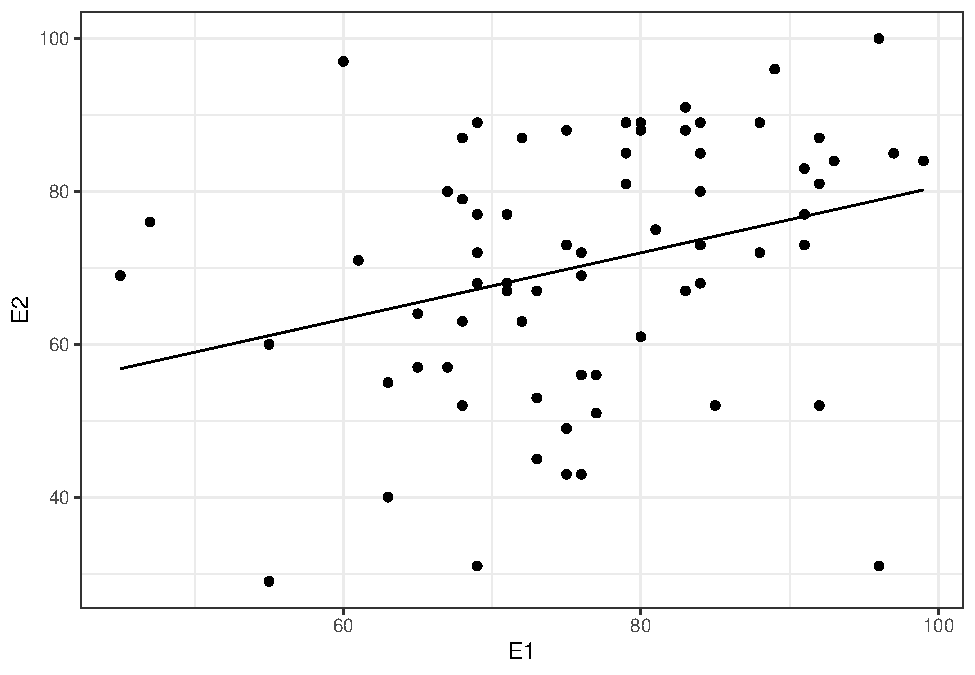
\includegraphics{_main_files/figure-latex/unnamed-chunk-75-1.pdf}

\begin{Shaded}
\begin{Highlighting}[]
\DocumentationTok{\#\# The basic output}
\NormalTok{Regfit }\OtherTok{\textless{}{-}} \FunctionTok{lm}\NormalTok{(E2 }\SpecialCharTok{\textasciitilde{}}\NormalTok{ E1)}
\FunctionTok{summary}\NormalTok{(Regfit)}
\end{Highlighting}
\end{Shaded}

\begin{verbatim}
## 
## Call:
## lm(formula = E2 ~ E1)
## 
## Residuals:
##     Min      1Q  Median      3Q     Max 
## -47.904  -9.123   2.178  12.218  33.693 
## 
## Coefficients:
##             Estimate Std. Error t value Pr(>|t|)   
## (Intercept)  37.3125    13.0485   2.860  0.00563 **
## E1            0.4332     0.1690   2.564  0.01256 * 
## ---
## Signif. codes:  0 '***' 0.001 '**' 0.01 '*' 0.05 '.' 0.1 ' ' 1
## 
## Residual standard error: 16.16 on 68 degrees of freedom
## Multiple R-squared:  0.08815,    Adjusted R-squared:  0.07474 
## F-statistic: 6.574 on 1 and 68 DF,  p-value: 0.01256
\end{verbatim}

Residuals \ldots{}

\begin{Shaded}
\begin{Highlighting}[]
\DocumentationTok{\#\# The two standard residual plots}
\FunctionTok{par}\NormalTok{(}\AttributeTok{mfrow =} \FunctionTok{c}\NormalTok{(}\DecValTok{1}\NormalTok{, }\DecValTok{2}\NormalTok{))}
\FunctionTok{plot}\NormalTok{(Regfit, }\DecValTok{1}\NormalTok{)}
\FunctionTok{plot}\NormalTok{(Regfit, }\DecValTok{2}\NormalTok{)}
\end{Highlighting}
\end{Shaded}

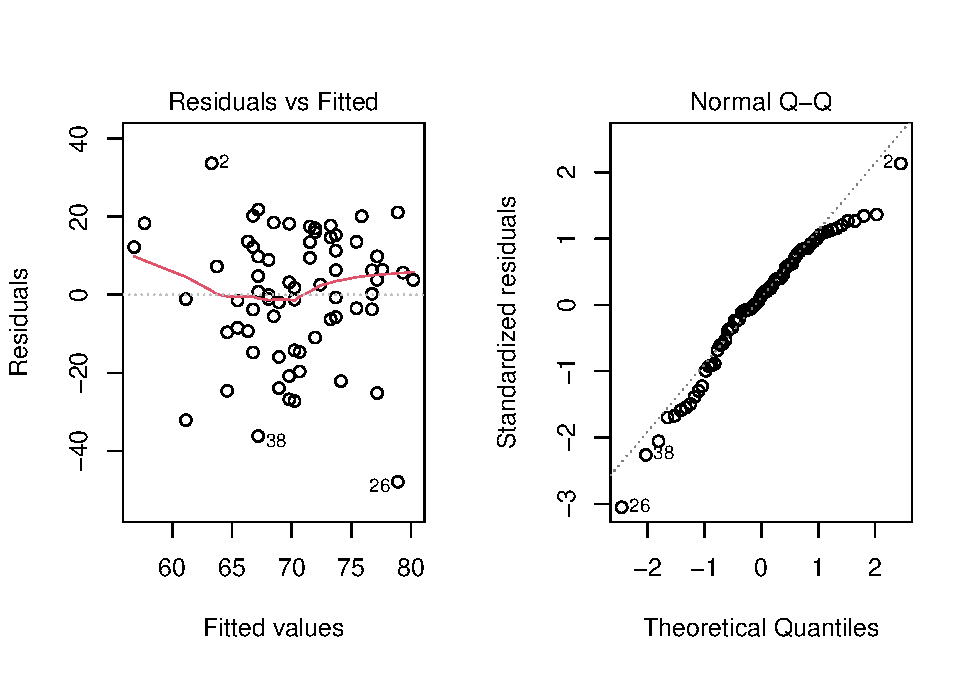
\includegraphics{_main_files/figure-latex/unnamed-chunk-76-1.pdf}

\begin{Shaded}
\begin{Highlighting}[]
\FunctionTok{par}\NormalTok{(}\AttributeTok{mfrow =} \FunctionTok{c}\NormalTok{(}\DecValTok{1}\NormalTok{, }\DecValTok{1}\NormalTok{))}

\DocumentationTok{\#\# The plots of the residuals vs. other variables to check independence. }
\DocumentationTok{\#\# Looks like the errors might have some dependence due to college.}
\NormalTok{residuals }\OtherTok{\textless{}{-}}\NormalTok{ Regfit}\SpecialCharTok{$}\NormalTok{residuals}
\FunctionTok{par}\NormalTok{(}\AttributeTok{mfrow =} \FunctionTok{c}\NormalTok{(}\DecValTok{2}\NormalTok{, }\DecValTok{2}\NormalTok{))}
\FunctionTok{plot}\NormalTok{(E3, residuals)}
\FunctionTok{lines}\NormalTok{(}\FunctionTok{c}\NormalTok{(}\SpecialCharTok{{-}}\FloatTok{1e10}\NormalTok{, }\FloatTok{1e10}\NormalTok{), }\FunctionTok{c}\NormalTok{(}\DecValTok{0}\NormalTok{, }\DecValTok{0}\NormalTok{))}
\FunctionTok{plot}\NormalTok{(Hmwk, residuals)}
\FunctionTok{lines}\NormalTok{(}\FunctionTok{c}\NormalTok{(}\SpecialCharTok{{-}}\FloatTok{1e10}\NormalTok{, }\FloatTok{1e10}\NormalTok{), }\FunctionTok{c}\NormalTok{(}\DecValTok{0}\NormalTok{, }\DecValTok{0}\NormalTok{))}
\FunctionTok{plot}\NormalTok{(}\FunctionTok{as.numeric}\NormalTok{(}\FunctionTok{as.factor}\NormalTok{(College)), residuals)}
\FunctionTok{lines}\NormalTok{(}\FunctionTok{c}\NormalTok{(}\SpecialCharTok{{-}}\FloatTok{1e10}\NormalTok{, }\FloatTok{1e10}\NormalTok{), }\FunctionTok{c}\NormalTok{(}\DecValTok{0}\NormalTok{, }\DecValTok{0}\NormalTok{))}
\FunctionTok{plot}\NormalTok{(Year, residuals)}
\FunctionTok{lines}\NormalTok{(}\FunctionTok{c}\NormalTok{(}\SpecialCharTok{{-}}\FloatTok{1e10}\NormalTok{, }\FloatTok{1e10}\NormalTok{), }\FunctionTok{c}\NormalTok{(}\DecValTok{0}\NormalTok{, }\DecValTok{0}\NormalTok{))}
\end{Highlighting}
\end{Shaded}

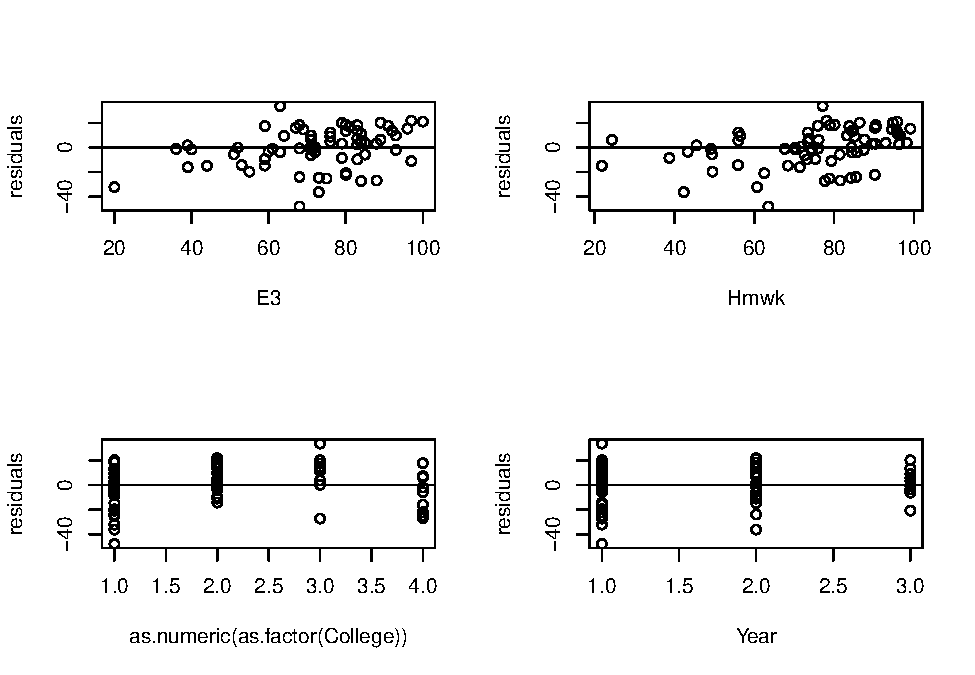
\includegraphics{_main_files/figure-latex/unnamed-chunk-76-2.pdf}

\begin{Shaded}
\begin{Highlighting}[]
\FunctionTok{par}\NormalTok{(}\AttributeTok{mfrow =} \FunctionTok{c}\NormalTok{(}\DecValTok{1}\NormalTok{, }\DecValTok{1}\NormalTok{))}
\end{Highlighting}
\end{Shaded}

The function \texttt{SASreg()} below will produce output similar to SAS using just one function. It requires that you have loaded in and installed the car package. To use it, simply copy the function in once, and then apply it to your data set.

\begin{Shaded}
\begin{Highlighting}[]
\NormalTok{SASreg }\OtherTok{\textless{}{-}} \ControlFlowTok{function}\NormalTok{(model) \{}
\NormalTok{  regout }\OtherTok{\textless{}{-}} \FunctionTok{lm}\NormalTok{(model)}
\NormalTok{  baseoutput }\OtherTok{\textless{}{-}} \FunctionTok{anova}\NormalTok{(regout)}
\NormalTok{  k }\OtherTok{\textless{}{-}} \FunctionTok{nrow}\NormalTok{(baseoutput) }\SpecialCharTok{{-}} \DecValTok{1}
\NormalTok{  Summary }\OtherTok{\textless{}{-}} \FunctionTok{round}\NormalTok{(}\FunctionTok{c}\NormalTok{(}
    \FunctionTok{summary}\NormalTok{(}\FunctionTok{lm}\NormalTok{(model))}\SpecialCharTok{$}\NormalTok{sigma,}
    \FunctionTok{summary}\NormalTok{(}\FunctionTok{lm}\NormalTok{(model))}\SpecialCharTok{$}\NormalTok{r.squared,}
    \FunctionTok{summary}\NormalTok{(}\FunctionTok{lm}\NormalTok{(model))}\SpecialCharTok{$}\NormalTok{adj.r.squared}
\NormalTok{  ), }\DecValTok{4}\NormalTok{)}
  \FunctionTok{names}\NormalTok{(Summary) }\OtherTok{\textless{}{-}} \FunctionTok{c}\NormalTok{(}\StringTok{"Root MSE"}\NormalTok{, }\StringTok{"R square"}\NormalTok{, }\StringTok{"Adj R{-}Squ"}\NormalTok{)}
\NormalTok{  ANOVA }\OtherTok{\textless{}{-}} \FunctionTok{rbind}\NormalTok{(}
    \FunctionTok{apply}\NormalTok{(baseoutput[}\DecValTok{1}\SpecialCharTok{:}\NormalTok{k, ], }\DecValTok{2}\NormalTok{, sum),}
\NormalTok{    baseoutput[k }\SpecialCharTok{+} \DecValTok{1}\NormalTok{, ],}
    \FunctionTok{apply}\NormalTok{(baseoutput[}\DecValTok{1}\SpecialCharTok{:}\NormalTok{(k }\SpecialCharTok{+} \DecValTok{1}\NormalTok{), ], }\DecValTok{2}\NormalTok{, sum)}
\NormalTok{  )}
  \FunctionTok{rownames}\NormalTok{(ANOVA) }\OtherTok{\textless{}{-}} \FunctionTok{c}\NormalTok{(}\StringTok{"Model"}\NormalTok{, }\StringTok{"Error"}\NormalTok{, }\StringTok{"C Total"}\NormalTok{)}
  \FunctionTok{attributes}\NormalTok{(ANOVA)}\SpecialCharTok{$}\NormalTok{heading }\OtherTok{\textless{}{-}} \FunctionTok{attributes}\NormalTok{(ANOVA)}\SpecialCharTok{$}\NormalTok{heading[}\DecValTok{1}\NormalTok{]}
\NormalTok{  ANOVA[}\DecValTok{1}\NormalTok{, }\DecValTok{3}\NormalTok{] }\OtherTok{\textless{}{-}}\NormalTok{ ANOVA[}\DecValTok{1}\NormalTok{, }\DecValTok{2}\NormalTok{] }\SpecialCharTok{/}\NormalTok{ ANOVA[}\DecValTok{1}\NormalTok{, }\DecValTok{1}\NormalTok{]}
\NormalTok{  ANOVA[}\DecValTok{1}\NormalTok{, }\DecValTok{4}\NormalTok{] }\OtherTok{\textless{}{-}}\NormalTok{ ANOVA[}\DecValTok{1}\NormalTok{, }\DecValTok{3}\NormalTok{] }\SpecialCharTok{/}\NormalTok{ ANOVA[}\DecValTok{2}\NormalTok{, }\DecValTok{3}\NormalTok{]}
\NormalTok{  ANOVA[}\DecValTok{1}\NormalTok{, }\DecValTok{5}\NormalTok{] }\OtherTok{\textless{}{-}} \DecValTok{1} \SpecialCharTok{{-}} \FunctionTok{pf}\NormalTok{(ANOVA[}\DecValTok{1}\NormalTok{, }\DecValTok{4}\NormalTok{], ANOVA[}\DecValTok{1}\NormalTok{, }\DecValTok{1}\NormalTok{], ANOVA[}\DecValTok{2}\NormalTok{, }\DecValTok{1}\NormalTok{])}
  \FunctionTok{attributes}\NormalTok{(ANOVA)}\SpecialCharTok{$}\NormalTok{heading }\OtherTok{\textless{}{-}} \ConstantTok{NULL}
\NormalTok{  TypeI }\OtherTok{\textless{}{-}}\NormalTok{ baseoutput[}\DecValTok{1}\SpecialCharTok{:}\NormalTok{k, ]}
  \FunctionTok{attributes}\NormalTok{(TypeI)}\SpecialCharTok{$}\NormalTok{heading }\OtherTok{\textless{}{-}} \ConstantTok{NULL}
\NormalTok{  TypeIII }\OtherTok{\textless{}{-}} \FunctionTok{Anova}\NormalTok{(regout, }\AttributeTok{type =} \DecValTok{3}\NormalTok{)[}\DecValTok{2}\SpecialCharTok{:}\NormalTok{(k }\SpecialCharTok{+} \DecValTok{1}\NormalTok{), }\FunctionTok{c}\NormalTok{(}\DecValTok{2}\NormalTok{, }\DecValTok{1}\NormalTok{, }\DecValTok{3}\NormalTok{, }\DecValTok{4}\NormalTok{)]}
  \FunctionTok{attributes}\NormalTok{(TypeIII)}\SpecialCharTok{$}\NormalTok{heading }\OtherTok{\textless{}{-}} \ConstantTok{NULL}
  \ControlFlowTok{if}\NormalTok{ (k }\SpecialCharTok{==} \DecValTok{1}\NormalTok{) \{}
\NormalTok{    vifs }\OtherTok{\textless{}{-}} \DecValTok{1}
\NormalTok{  \} }\ControlFlowTok{else}\NormalTok{ \{}
\NormalTok{    vifs }\OtherTok{\textless{}{-}} \FunctionTok{t}\NormalTok{(}\FunctionTok{vif}\NormalTok{(regout))}
\NormalTok{  \}}
\NormalTok{  ParEsts }\OtherTok{\textless{}{-}} \FunctionTok{round}\NormalTok{(}\FunctionTok{cbind}\NormalTok{(}\FunctionTok{summary}\NormalTok{(regout)}\SpecialCharTok{$}\NormalTok{coefficients, }\FunctionTok{c}\NormalTok{(}\DecValTok{0}\NormalTok{, vifs)), }\DecValTok{4}\NormalTok{)}
  \FunctionTok{colnames}\NormalTok{(ParEsts)[}\DecValTok{5}\NormalTok{] }\OtherTok{\textless{}{-}} \StringTok{"VIF"}
  \FunctionTok{par}\NormalTok{(}\AttributeTok{mfrow =} \FunctionTok{c}\NormalTok{(}\DecValTok{1}\NormalTok{, }\DecValTok{2}\NormalTok{))}
  \FunctionTok{plot}\NormalTok{(regout}\SpecialCharTok{$}\NormalTok{fitted.values, regout}\SpecialCharTok{$}\NormalTok{residuals, }\AttributeTok{xlab =} \StringTok{"Fitted"}\NormalTok{, }\AttributeTok{ylab =} \StringTok{"Residuals"}\NormalTok{)}
  \FunctionTok{lines}\NormalTok{(}\FunctionTok{c}\NormalTok{(}\FunctionTok{min}\NormalTok{(regout}\SpecialCharTok{$}\NormalTok{fitted.values) }\SpecialCharTok{{-}} \DecValTok{1}\NormalTok{, }\FunctionTok{max}\NormalTok{(regout}\SpecialCharTok{$}\NormalTok{fitted.values) }\SpecialCharTok{+} \DecValTok{1}\NormalTok{), }\FunctionTok{c}\NormalTok{(}\DecValTok{0}\NormalTok{, }\DecValTok{0}\NormalTok{))}
  \FunctionTok{qqnorm}\NormalTok{(regout}\SpecialCharTok{$}\NormalTok{residuals)}
  \FunctionTok{qqline}\NormalTok{(regout}\SpecialCharTok{$}\NormalTok{residuals)}
  \FunctionTok{par}\NormalTok{(}\AttributeTok{mfrow =} \FunctionTok{c}\NormalTok{(}\DecValTok{1}\NormalTok{, }\DecValTok{1}\NormalTok{))}
  \FunctionTok{list}\NormalTok{(}
    \AttributeTok{Model.Equation =}\NormalTok{ model,}
    \AttributeTok{Coefficients =}\NormalTok{ regout}\SpecialCharTok{$}\NormalTok{coefficients,}
    \AttributeTok{Summary =}\NormalTok{ Summary,}
    \AttributeTok{Analysis.of.Variance =}\NormalTok{ ANOVA,}
    \AttributeTok{Type.I.Tests =}\NormalTok{ TypeI,}
    \AttributeTok{Type.III.Tests =}\NormalTok{ TypeIII,}
    \AttributeTok{Parameter.Estimates =}\NormalTok{ ParEsts}
\NormalTok{  )}
\NormalTok{\}}


\FunctionTok{SASreg}\NormalTok{(E2 }\SpecialCharTok{\textasciitilde{}}\NormalTok{ E1)}
\end{Highlighting}
\end{Shaded}

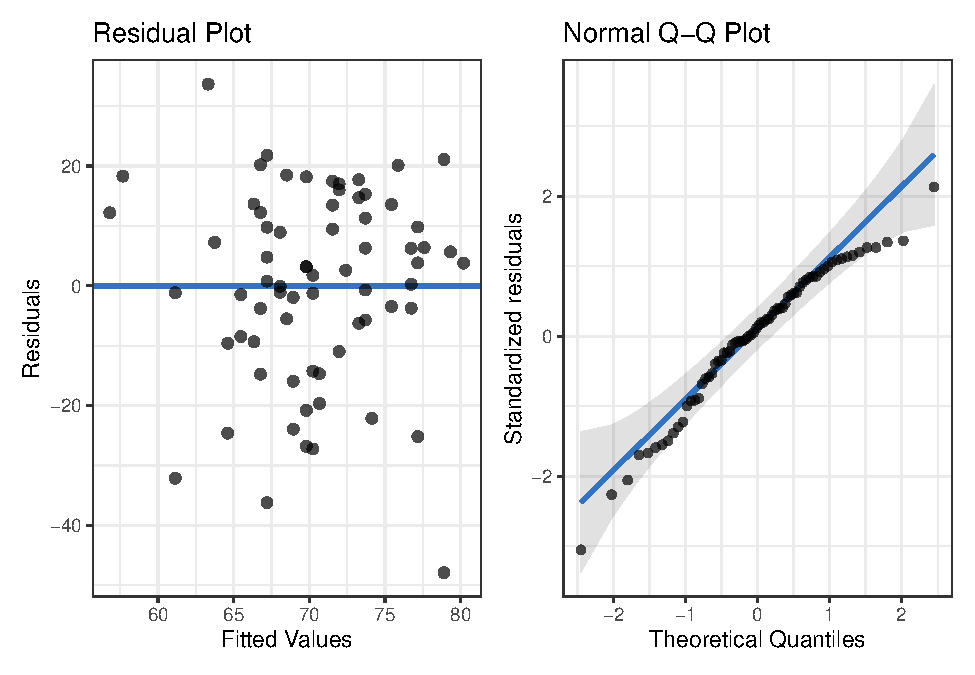
\includegraphics{_main_files/figure-latex/unnamed-chunk-77-1.pdf}

\begin{verbatim}
## $Model.Equation
## E2 ~ E1
## 
## $Coefficients
## (Intercept)          E1 
##  37.3125215   0.4332442 
## 
## $Summary
##  Root MSE  R square Adj R-Squ 
##   16.1601    0.0882    0.0747 
## 
## $Analysis.of.Variance
##         Df  Sum Sq Mean Sq F value  Pr(>F)  
## Model    1  1716.8 1716.77   6.574 0.01256 *
## Error   68 17758.0  261.15                  
## C Total 69 19474.8 1977.92                  
## ---
## Signif. codes:  0 '***' 0.001 '**' 0.01 '*' 0.05 '.' 0.1 ' ' 1
## 
## $Type.I.Tests
##    Df Sum Sq Mean Sq F value  Pr(>F)  
## E1  1 1716.8  1716.8   6.574 0.01256 *
## ---
## Signif. codes:  0 '***' 0.001 '**' 0.01 '*' 0.05 '.' 0.1 ' ' 1
## 
## $Type.III.Tests
##    Df Sum Sq F value  Pr(>F)  
## E1  1 1716.8   6.574 0.01256 *
## ---
## Signif. codes:  0 '***' 0.001 '**' 0.01 '*' 0.05 '.' 0.1 ' ' 1
## 
## $Parameter.Estimates
##             Estimate Std. Error t value Pr(>|t|) VIF
## (Intercept)  37.3125    13.0485  2.8595   0.0056   0
## E1            0.4332     0.1690  2.5640   0.0126   1
\end{verbatim}

This output is perhaps a bit overkill for simple linear regression, but is very useful when performing multiple regression (or even ANCOVA or factorial ANOVA).

\hypertarget{box-cox-transformation}{%
\subsection{Box-Cox Transformation}\label{box-cox-transformation}}

To get the Box-Cox transformation for this data set we could use the boxcox function from the MASS library (which is automatically included with R and just needs to have library(MASS) to install:

\begin{Shaded}
\begin{Highlighting}[]
\FunctionTok{library}\NormalTok{(MASS)}
\FunctionTok{boxcox}\NormalTok{(}\FunctionTok{lm}\NormalTok{(E2 }\SpecialCharTok{\textasciitilde{}}\NormalTok{ E1))}
\end{Highlighting}
\end{Shaded}

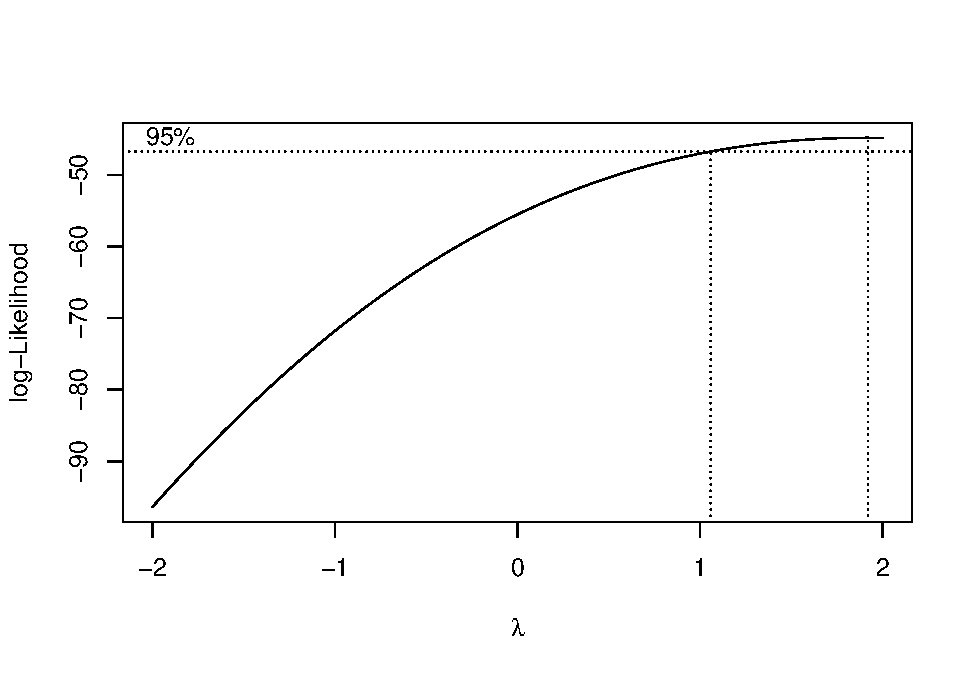
\includegraphics{_main_files/figure-latex/unnamed-chunk-78-1.pdf}

This plot doesn't have the peak! So try from \texttt{0} to \texttt{5} with spacing every \texttt{.01} to see if its better:

\begin{Shaded}
\begin{Highlighting}[]
\FunctionTok{boxcox}\NormalTok{(}\FunctionTok{lm}\NormalTok{(E2 }\SpecialCharTok{\textasciitilde{}}\NormalTok{ E1), }\AttributeTok{lambda =} \FunctionTok{seq}\NormalTok{(}\DecValTok{0}\NormalTok{, }\DecValTok{5}\NormalTok{, .}\DecValTok{01}\NormalTok{))}
\end{Highlighting}
\end{Shaded}

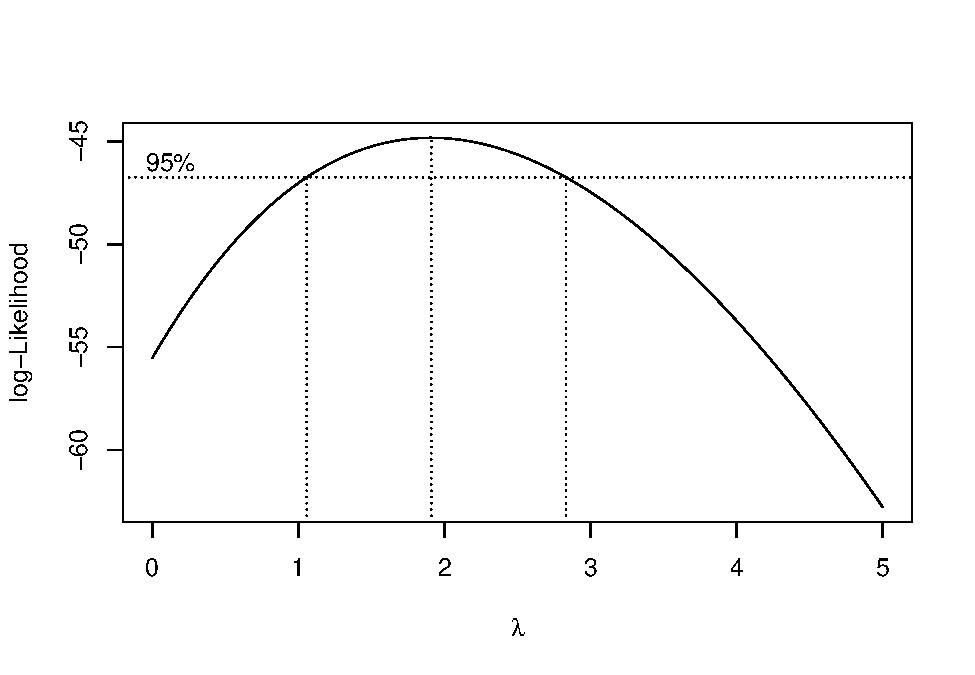
\includegraphics{_main_files/figure-latex/unnamed-chunk-79-1.pdf}

It looks like 1 is just outside the range, of the values that make the 95\% cut-off, the one that is ``nicest'' and close to the peak is 2. So, the transformation y-squared is recommended.

\hypertarget{multiple-linear-regression}{%
\subsection{Multiple Linear Regression}\label{multiple-linear-regression}}

Predict the performance on Exam3 from the performance of the first two exams and the homework.

This can be done by mimicking the procedure for simple linear regression. In this case the model statement must be of the form \texttt{E3\ \textasciitilde{}\ Hmwk\ +\ E1\ +\ E2}. An interaction could be added by something like \texttt{+\ E2*E3} if it were needed.

\begin{Shaded}
\begin{Highlighting}[]
\FunctionTok{SASreg}\NormalTok{(E3 }\SpecialCharTok{\textasciitilde{}}\NormalTok{ Hmwk }\SpecialCharTok{+}\NormalTok{ E1 }\SpecialCharTok{+}\NormalTok{ E2)}
\end{Highlighting}
\end{Shaded}

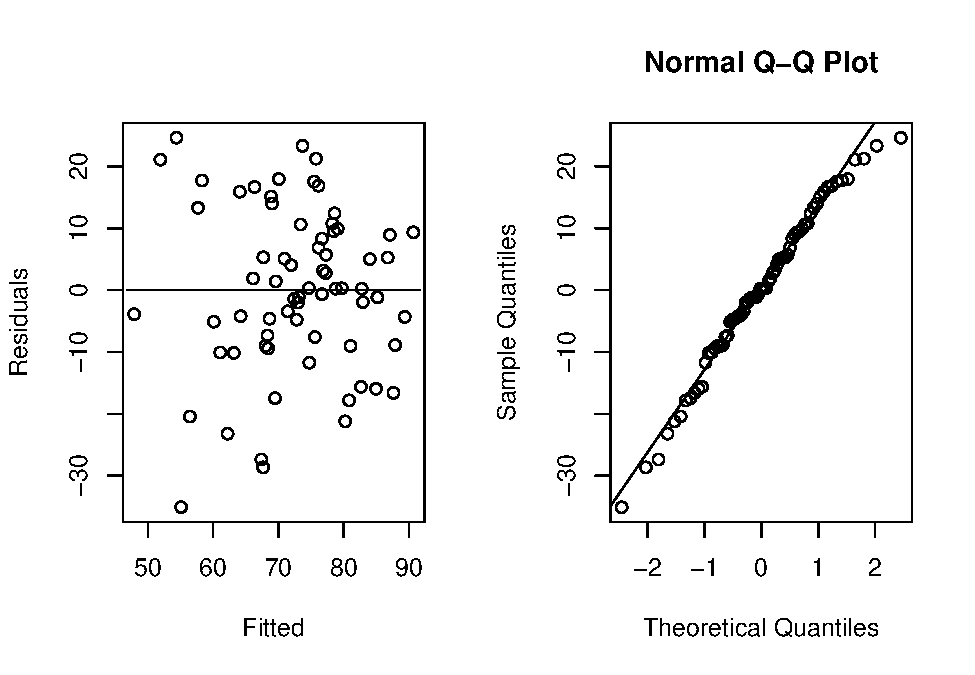
\includegraphics{_main_files/figure-latex/unnamed-chunk-80-1.pdf}

\begin{verbatim}
## $Model.Equation
## E3 ~ Hmwk + E1 + E2
## 
## $Coefficients
## (Intercept)        Hmwk          E1          E2 
##  14.3989784   0.3708761   0.2345946   0.1820907 
## 
## $Summary
##  Root MSE  R square Adj R-Squ 
##   13.4719    0.3425    0.3126 
## 
## $Analysis.of.Variance
##         Df  Sum Sq Mean Sq F value    Pr(>F)    
## Model    3  6239.5  2079.8   11.46 3.859e-06 ***
## Error   66 11978.5   181.5                      
## C Total 69 18218.0  6421.0                      
## ---
## Signif. codes:  0 '***' 0.001 '**' 0.01 '*' 0.05 '.' 0.1 ' ' 1
## 
## $Type.I.Tests
##      Df Sum Sq Mean Sq F value   Pr(>F)    
## Hmwk  1 5047.1  5047.1 27.8092 1.59e-06 ***
## E1    1  688.8   688.8  3.7955  0.05565 .  
## E2    1  503.5   503.5  2.7743  0.10053    
## ---
## Signif. codes:  0 '***' 0.001 '**' 0.01 '*' 0.05 '.' 0.1 ' ' 1
## 
## $Type.III.Tests
##      Df  Sum Sq F value    Pr(>F)    
## Hmwk  1 2290.06 12.6179 0.0007109 ***
## E1    1  445.25  2.4533 0.1220639    
## E2    1  503.51  2.7743 0.1005295    
## ---
## Signif. codes:  0 '***' 0.001 '**' 0.01 '*' 0.05 '.' 0.1 ' ' 1
## 
## $Parameter.Estimates
##             Estimate Std. Error t value Pr(>|t|)    VIF
## (Intercept)  14.3990    11.8819  1.2118   0.2299 0.0000
## Hmwk          0.3709     0.1044  3.5522   0.0007 1.2667
## E1            0.2346     0.1498  1.5663   0.1221 1.1305
## E2            0.1821     0.1093  1.6656   0.1005 1.2824
\end{verbatim}

The plots to help assess independence (the residuals versus other variables not included in the model) and to check for needing higher order terms (the residual versus independent variables) could be generated as follows:

\begin{Shaded}
\begin{Highlighting}[]
\NormalTok{residuals }\OtherTok{\textless{}{-}} \FunctionTok{lm}\NormalTok{(E3 }\SpecialCharTok{\textasciitilde{}}\NormalTok{ Hmwk }\SpecialCharTok{+}\NormalTok{ E1 }\SpecialCharTok{+}\NormalTok{ E2)}\SpecialCharTok{$}\NormalTok{residuals}

\DocumentationTok{\#\# Sign of non{-}constant variance based on College?}
\FunctionTok{par}\NormalTok{(}\AttributeTok{mfrow =} \FunctionTok{c}\NormalTok{(}\DecValTok{1}\NormalTok{, }\DecValTok{2}\NormalTok{))}
\FunctionTok{plot}\NormalTok{(}\FunctionTok{as.numeric}\NormalTok{(}\FunctionTok{as.factor}\NormalTok{(College)), residuals)}
\FunctionTok{plot}\NormalTok{(Year, residuals)}
\end{Highlighting}
\end{Shaded}

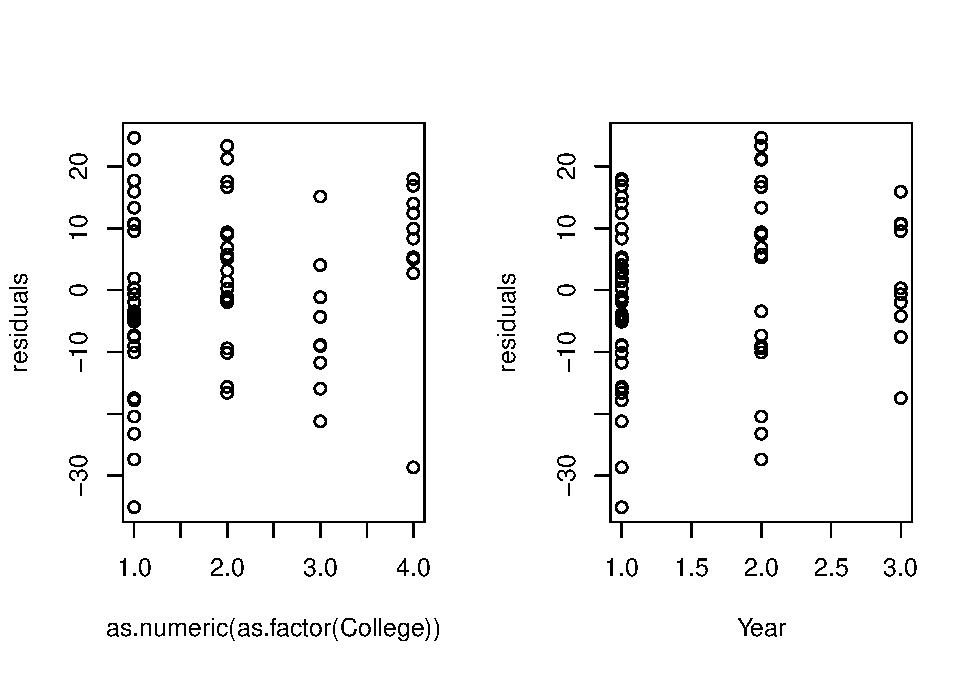
\includegraphics{_main_files/figure-latex/unnamed-chunk-81-1.pdf}

\begin{Shaded}
\begin{Highlighting}[]
\FunctionTok{par}\NormalTok{(}\AttributeTok{mfrow =} \FunctionTok{c}\NormalTok{(}\DecValTok{1}\NormalTok{, }\DecValTok{1}\NormalTok{))}

\DocumentationTok{\#\# Plotting against group might be better}
\FunctionTok{plot}\NormalTok{(grp, residuals)}
\end{Highlighting}
\end{Shaded}

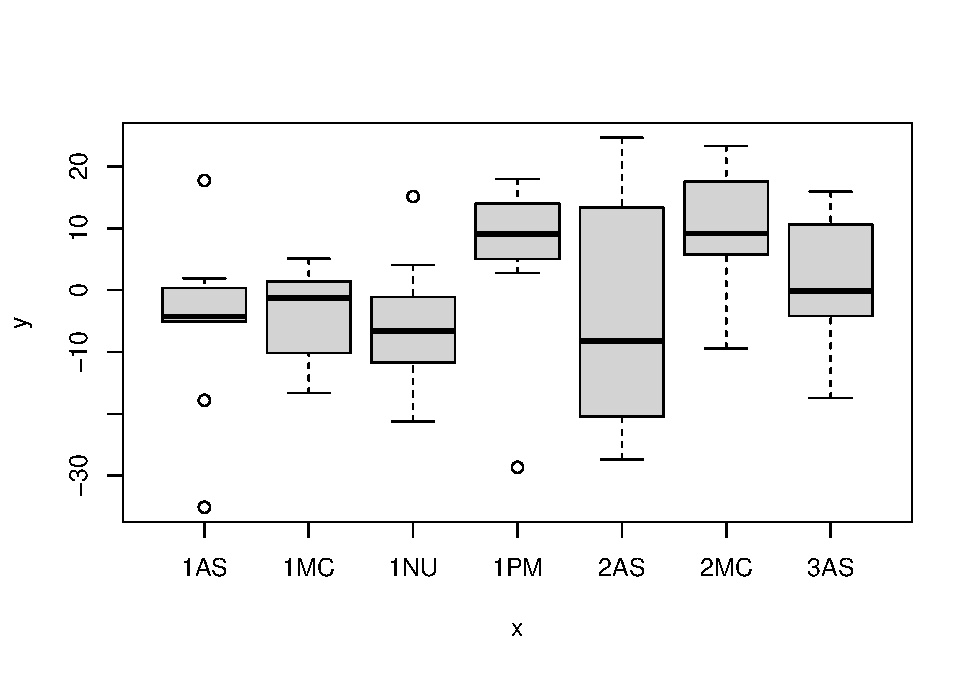
\includegraphics{_main_files/figure-latex/unnamed-chunk-81-2.pdf}

\begin{Shaded}
\begin{Highlighting}[]
\DocumentationTok{\#\# No signs of needing higher order terms}
\FunctionTok{par}\NormalTok{(}\AttributeTok{mfrow =} \FunctionTok{c}\NormalTok{(}\DecValTok{2}\NormalTok{, }\DecValTok{2}\NormalTok{))}
\FunctionTok{plot}\NormalTok{(Hmwk, residuals)}
\FunctionTok{plot}\NormalTok{(E1, residuals)}
\FunctionTok{plot}\NormalTok{(E2, residuals)}
\FunctionTok{par}\NormalTok{(}\AttributeTok{mfrow =} \FunctionTok{c}\NormalTok{(}\DecValTok{1}\NormalTok{, }\DecValTok{1}\NormalTok{))}
\end{Highlighting}
\end{Shaded}

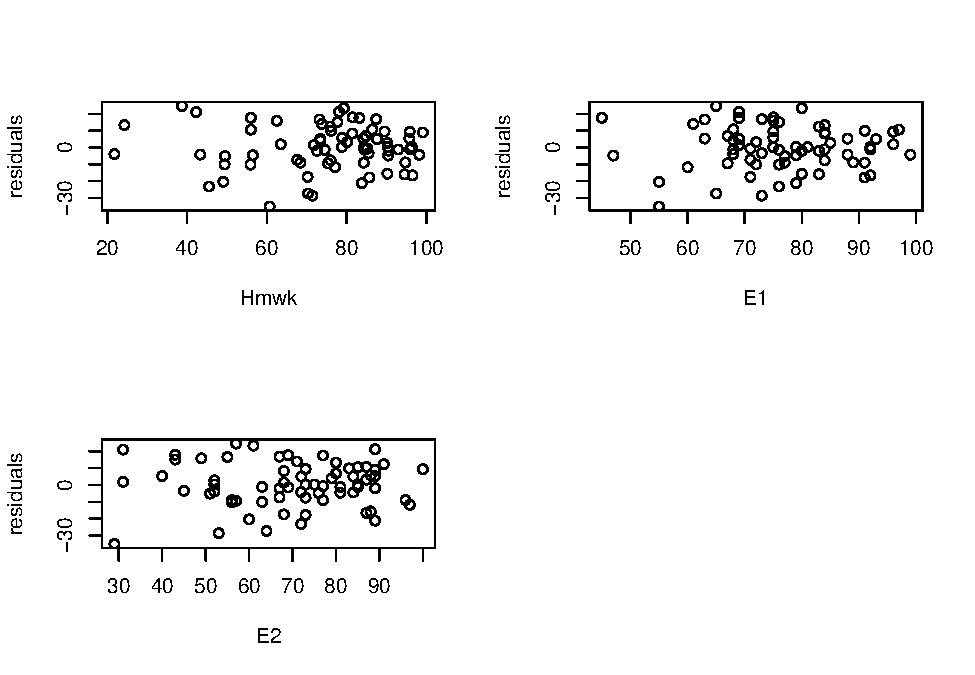
\includegraphics{_main_files/figure-latex/unnamed-chunk-81-3.pdf}

\hypertarget{variable-selection}{%
\subsection{Variable Selection}\label{variable-selection}}

Assuming we trusted the model fit, is there a subset of Hmwk, E1, and E2 that predicts E3 just as well as all three of them?

R has some packages that do all subsets variable selection, but the output is somewhat inelegant. The Cp function below is a bit prettier. It requires the leaps library, and that package must be installed for it to run It also requires that you put all of the predictor variables together in a matrix called X. To run it, be sure to load the \textbf{leaps} library and copy over the function, construct the \texttt{X} matrix using \texttt{cbind()}, and then run the function.

\begin{Shaded}
\begin{Highlighting}[]
\FunctionTok{library}\NormalTok{(leaps)}
\NormalTok{Cp }\OtherTok{\textless{}{-}} \ControlFlowTok{function}\NormalTok{(X, Y) \{}
\NormalTok{  baseout }\OtherTok{\textless{}{-}} \FunctionTok{summary}\NormalTok{(}\FunctionTok{regsubsets}\NormalTok{(X, Y, }\AttributeTok{nbest =} \DecValTok{10}\NormalTok{))}
\NormalTok{  inmat }\OtherTok{\textless{}{-}}\NormalTok{ baseout}\SpecialCharTok{$}\NormalTok{which[, }\SpecialCharTok{{-}}\DecValTok{1}\NormalTok{]}
\NormalTok{  n }\OtherTok{\textless{}{-}} \FunctionTok{nrow}\NormalTok{(inmat)}
\NormalTok{  namemat }\OtherTok{\textless{}{-}} \FunctionTok{matrix}\NormalTok{(}\FunctionTok{rep}\NormalTok{(}\FunctionTok{colnames}\NormalTok{(X), n), }\AttributeTok{nrow =}\NormalTok{ n, }\AttributeTok{byrow =}\NormalTok{ T)}
\NormalTok{  namemat[}\SpecialCharTok{!}\NormalTok{inmat] }\OtherTok{\textless{}{-}} \StringTok{""}
\NormalTok{  namemat }\OtherTok{\textless{}{-}} \FunctionTok{cbind}\NormalTok{(}\FunctionTok{rep}\NormalTok{(}\StringTok{" "}\NormalTok{, n), namemat)}
\NormalTok{  nvars }\OtherTok{\textless{}{-}} \FunctionTok{apply}\NormalTok{(inmat, }\DecValTok{1}\NormalTok{, sum)}
\NormalTok{  sets }\OtherTok{\textless{}{-}} \FunctionTok{apply}\NormalTok{(namemat, }\DecValTok{1}\NormalTok{, paste, }\AttributeTok{collapse =} \StringTok{" "}\NormalTok{)}
  \ControlFlowTok{for}\NormalTok{ (i }\ControlFlowTok{in} \DecValTok{1}\SpecialCharTok{:}\FunctionTok{ncol}\NormalTok{(X)) \{}
\NormalTok{    sets }\OtherTok{\textless{}{-}} \FunctionTok{gsub}\NormalTok{(}\StringTok{"  "}\NormalTok{, }\StringTok{" "}\NormalTok{, sets)}
\NormalTok{  \}}
\NormalTok{  out }\OtherTok{\textless{}{-}} \FunctionTok{as.table}\NormalTok{(}\FunctionTok{cbind}\NormalTok{(}
\NormalTok{    sets, }\FunctionTok{round}\NormalTok{(baseout}\SpecialCharTok{$}\NormalTok{cp, }\DecValTok{4}\NormalTok{),}
    \FunctionTok{round}\NormalTok{(baseout}\SpecialCharTok{$}\NormalTok{rsq, }\DecValTok{4}\NormalTok{), }\FunctionTok{round}\NormalTok{(baseout}\SpecialCharTok{$}\NormalTok{adjr2, }\DecValTok{4}\NormalTok{)}
\NormalTok{  ))}
  \FunctionTok{colnames}\NormalTok{(out) }\OtherTok{\textless{}{-}} \FunctionTok{c}\NormalTok{(}\StringTok{"Variables"}\NormalTok{, }\StringTok{"Cp"}\NormalTok{, }\StringTok{"R square"}\NormalTok{, }\StringTok{"adj{-}R2"}\NormalTok{)}
  \FunctionTok{rownames}\NormalTok{(out) }\OtherTok{\textless{}{-}}\NormalTok{ nvars}
\NormalTok{  out}
\NormalTok{\}}

\NormalTok{X }\OtherTok{\textless{}{-}} \FunctionTok{cbind}\NormalTok{(Hmwk, E1, E2)}
\FunctionTok{Cp}\NormalTok{(X, E3)}
\end{Highlighting}
\end{Shaded}

\begin{verbatim}
##   Variables   Cp      R square adj-R2
## 1  Hmwk       6.5697  0.277    0.2664
## 1  E2         17.5215 0.1679   0.1557
## 1  E1         23.2662 0.1107   0.0976
## 2  Hmwk E2    4.4533  0.3181   0.2977
## 2  Hmwk E1    4.7743  0.3149   0.2944
## 2  E1 E2      14.6179 0.2168   0.1934
## 3  Hmwk E1 E2 4       0.3425   0.3126
\end{verbatim}

It looks as if using Hmwk and just one of the other two exams just misses the general guideline for Mallow's Cp, and have slightly worse adjusted R-squared values.

\hypertarget{outlier-diagnostics}{%
\subsection{Outlier Diagnostics}\label{outlier-diagnostics}}

Are there examinees that are either extreme in terms of their predictor variables, have E3 badly predicted by the model, or significantly change the model?

R has the built in functions hatvalues, rstudent, dffits, and cooks.distance to help with outlier diagnsostics. The function outlier below puts them into one a single matrix.

\begin{Shaded}
\begin{Highlighting}[]
\NormalTok{outlier }\OtherTok{\textless{}{-}} \ControlFlowTok{function}\NormalTok{(model) \{}
\NormalTok{  baseout }\OtherTok{\textless{}{-}} \FunctionTok{lm}\NormalTok{(model)}
\NormalTok{  outs }\OtherTok{\textless{}{-}} \FunctionTok{cbind}\NormalTok{(}
    \FunctionTok{hatvalues}\NormalTok{(baseout), }\FunctionTok{rstudent}\NormalTok{(baseout),}
    \FunctionTok{dffits}\NormalTok{(baseout), }\FunctionTok{cooks.distance}\NormalTok{(baseout)}
\NormalTok{  )}
\NormalTok{  outs }\OtherTok{\textless{}{-}} \FunctionTok{round}\NormalTok{(outs, }\DecValTok{4}\NormalTok{)}
  \FunctionTok{colnames}\NormalTok{(outs) }\OtherTok{\textless{}{-}} \FunctionTok{c}\NormalTok{(}\StringTok{"hii"}\NormalTok{, }\StringTok{"ti"}\NormalTok{, }\StringTok{"DFFITS"}\NormalTok{, }\StringTok{"Cooks.D"}\NormalTok{)}
\NormalTok{  outs}
\NormalTok{\}}

\FunctionTok{outlier}\NormalTok{(E3 }\SpecialCharTok{\textasciitilde{}}\NormalTok{ Hmwk }\SpecialCharTok{+}\NormalTok{ E1 }\SpecialCharTok{+}\NormalTok{ E2)}
\end{Highlighting}
\end{Shaded}

\begin{verbatim}
##       hii      ti  DFFITS Cooks.D
## 1  0.0322 -1.6206 -0.2957  0.0213
## 2  0.1088 -0.9214 -0.3219  0.0260
## 3  0.0382 -1.2109 -0.2413  0.0145
## 4  0.0382 -0.6809 -0.1357  0.0046
## 5  0.0309  0.3026  0.0541  0.0007
## 6  0.0569 -0.6760 -0.1660  0.0069
## 7  0.0672  1.1656  0.3127  0.0243
## 8  0.0474 -0.0895 -0.0200  0.0001
## 9  0.0381 -0.0864 -0.0172  0.0001
## 10 0.0798 -0.3335 -0.0982  0.0024
## 11 0.0308 -2.2243 -0.3966  0.0371
## 12 0.1040  0.4138  0.1410  0.0050
## 13 0.0747  0.2098  0.0596  0.0009
## 14 0.0242  0.6225  0.0980  0.0024
## 15 0.0434  1.0629  0.2264  0.0128
## 16 0.0736  1.3942  0.3930  0.0381
## 17 0.0434  0.7501  0.1598  0.0064
## 18 0.0473  0.3777  0.0842  0.0018
## 19 0.0283  1.2757  0.2177  0.0117
## 20 0.0418  0.9402  0.1962  0.0096
## 21 0.1257 -2.9432 -1.1158  0.2789
## 22 0.1501 -0.3123 -0.1312  0.0044
## 23 0.0557 -0.3876 -0.0942  0.0022
## 24 0.0406 -1.3594 -0.2795  0.0193
## 25 0.0533 -0.3513 -0.0833  0.0018
## 26 0.1857  0.1539  0.0735  0.0014
## 27 0.1523 -0.3838 -0.1627  0.0067
## 28 0.0797  0.0249  0.0073  0.0000
## 29 0.1372  1.4264  0.5689  0.0797
## 30 0.0276  0.0167  0.0028  0.0000
## 31 0.0808 -1.6009 -0.4747  0.0550
## 32 0.0286 -2.1151 -0.3627  0.0312
## 33 0.0692 -1.8169 -0.4953  0.0593
## 34 0.0464 -0.7640 -0.1685  0.0071
## 35 0.0265 -0.6764 -0.1117  0.0031
## 36 0.0189 -0.5461 -0.0758  0.0015
## 37 0.0751 -0.2627 -0.0749  0.0014
## 38 0.1081  1.6797  0.5848  0.0832
## 39 0.2150  1.1177  0.5849  0.0852
## 40 0.0805  1.9456  0.5756  0.0795
## 41 0.0179 -1.3160 -0.1775  0.0078
## 42 0.1048 -0.3283 -0.1123  0.0032
## 43 0.0209 -0.5660 -0.0828  0.0017
## 44 0.0218 -0.1487 -0.0222  0.0001
## 45 0.0265 -0.0504 -0.0083  0.0000
## 46 0.0397  1.2089  0.2459  0.0150
## 47 0.0257  0.0215  0.0035  0.0000
## 48 0.1169  0.8353  0.3040  0.0232
## 49 0.0263  0.7135  0.1172  0.0035
## 50 0.0477  0.8166  0.1828  0.0084
## 51 0.0365 -0.7657 -0.1490  0.0056
## 52 0.0333 -1.1846 -0.2197  0.0120
## 53 0.0350 -0.0844 -0.0161  0.0001
## 54 0.0203  0.1044  0.0150  0.0001
## 55 0.0144 -0.1056 -0.0128  0.0000
## 56 0.0535 -1.2735 -0.3029  0.0227
## 57 0.0215  0.3788  0.0562  0.0008
## 58 0.0357  0.2372  0.0456  0.0005
## 59 0.0350 -0.1453 -0.0277  0.0002
## 60 0.0369  0.0170  0.0033  0.0000
## 61 0.0325 -0.7084 -0.1298  0.0042
## 62 0.0424  1.2695  0.2672  0.0177
## 63 0.0384  0.5168  0.1033  0.0027
## 64 0.0336  0.4293  0.0801  0.0016
## 65 0.0288  1.3285  0.2288  0.0129
## 66 0.0458  0.3970  0.0869  0.0019
## 67 0.0255  1.7818  0.2880  0.0201
## 68 0.0474  1.6359  0.3649  0.0325
## 69 0.0467  0.6765  0.1498  0.0057
## 70 0.0824  0.7212  0.2162  0.0118
\end{verbatim}

\hypertarget{prediction-intervals-and-confidence-intervals-for-the-regression-line}{%
\subsection{Prediction Intervals and Confidence Intervals for the Regression Line}\label{prediction-intervals-and-confidence-intervals-for-the-regression-line}}

What is the confidence interval for the mean E3 scores for examinees with Hmwk=95, E1=70, and E2=85? What would the prediction interval be?

The prediction intervals and confidence intervals for the regression surface can be gotten using the built in predict function. The following give those intervals for data points matching the original data (again using the model we defined above):

\begin{verbatim}
predict(lm(E3~Hmwk+E1+E2),interval="confidence")
predict(lm(E3~Hmwk+E1+E2),interval="predict")
\end{verbatim}

For Hmwk=95, E1=70, and E2=85:

\begin{verbatim}
predict(lm(E3~Hmwk+E1+E2),data.frame(Hmwk=95,E1=70,E2=85),interval="confidence")
predict(lm(E3~Hmwk+E1+E2),data.frame(Hmwk=95,E1=70,E2=85),interval="predict")
\end{verbatim}

\hypertarget{factorial-anova}{%
\subsection{Factorial ANOVA}\label{factorial-anova}}

Conduct a 2-way ANOVA for Hmwk based on Year 1 vs.~2 and AS vs.~MC.

The data for this problem can be constructed using:

\begin{verbatim}
HmwkA<-Hmwk[((College=="AS")|(College=="MC"))&((Year==1)|(Year==2))]
CollegeA<-College[((College=="AS")|(College=="MC"))&((Year==1)|(Year==2))]
CollegeA<-as.factor(as.character(CollegeA))
YearA<-Year[((College=="AS")|(College=="MC"))&((Year==1)|(Year==2))]
YearA<-as.factor(as.character(YearA))
\end{verbatim}

The basic output can again be constructed either using the built in functions or SASreg. The interaction is added using a colon if the terms are listed separately, or all the terms will be crossed using an asterisk.

\begin{verbatim}
summary(lm(HmwkA~CollegeA+YearA+CollegeA:YearA))
par(mfrow=c(1,2))
plot(lm(HmwkA~CollegeA+YearA+CollegeA:YearA),1)
plot(lm(HmwkA~CollegeA+YearA+CollegeA:YearA),2)
par(mfrow=c(1,1))

SASreg(HmwkA~CollegeA+YearA+CollegeA:YearA)
SASreg(HmwkA~CollegeA*YearA)
\end{verbatim}

Profile plots can be constructed using the built in function interaction.plot. The first argument is the variable on the x-axis, and the third is the response variable.

\begin{verbatim}
interaction.plot(CollegeA,YearA,HmwkA)
interaction.plot(YearA,CollegeA,HmwkA)
\end{verbatim}

\hypertarget{ancova}{%
\subsection{ANCOVA}\label{ancova}}

Predict E3 from Hmwk using grp as a covariate.

Again this can be performed using either the built in functions or SASreg.

\begin{Shaded}
\begin{Highlighting}[]
\FunctionTok{summary}\NormalTok{(}\FunctionTok{lm}\NormalTok{(E3 }\SpecialCharTok{\textasciitilde{}}\NormalTok{ Hmwk }\SpecialCharTok{+}\NormalTok{ grp))}
\end{Highlighting}
\end{Shaded}

\begin{verbatim}
## 
## Call:
## lm(formula = E3 ~ Hmwk + grp)
## 
## Residuals:
##     Min      1Q  Median      3Q     Max 
## -39.791  -5.051   1.322   7.752  25.999 
## 
## Coefficients:
##             Estimate Std. Error t value Pr(>|t|)    
## (Intercept) 41.28345    8.50894   4.852  8.6e-06 ***
## Hmwk         0.30491    0.11446   2.664 0.009829 ** 
## grp1MC       6.40928    6.03209   1.063 0.292116    
## grp1NU       7.61338    6.27024   1.214 0.229273    
## grp1PM      15.03430    6.01798   2.498 0.015147 *  
## grp2AS      -0.08199    5.88744  -0.014 0.988934    
## grp2MC      21.30066    6.14449   3.467 0.000963 ***
## grp3AS      11.37722    5.80620   1.959 0.054554 .  
## ---
## Signif. codes:  0 '***' 0.001 '**' 0.01 '*' 0.05 '.' 0.1 ' ' 1
## 
## Residual standard error: 12.85 on 62 degrees of freedom
## Multiple R-squared:  0.4382, Adjusted R-squared:  0.3748 
## F-statistic: 6.909 on 7 and 62 DF,  p-value: 4.48e-06
\end{verbatim}

\begin{Shaded}
\begin{Highlighting}[]
\FunctionTok{par}\NormalTok{(}\AttributeTok{mfrow =} \FunctionTok{c}\NormalTok{(}\DecValTok{1}\NormalTok{, }\DecValTok{2}\NormalTok{))}
\FunctionTok{plot}\NormalTok{(}\FunctionTok{lm}\NormalTok{(E3 }\SpecialCharTok{\textasciitilde{}}\NormalTok{ Hmwk }\SpecialCharTok{+}\NormalTok{ grp), }\DecValTok{1}\NormalTok{)}
\FunctionTok{plot}\NormalTok{(}\FunctionTok{lm}\NormalTok{(E3 }\SpecialCharTok{\textasciitilde{}}\NormalTok{ Hmwk }\SpecialCharTok{+}\NormalTok{ grp), }\DecValTok{2}\NormalTok{)}
\end{Highlighting}
\end{Shaded}

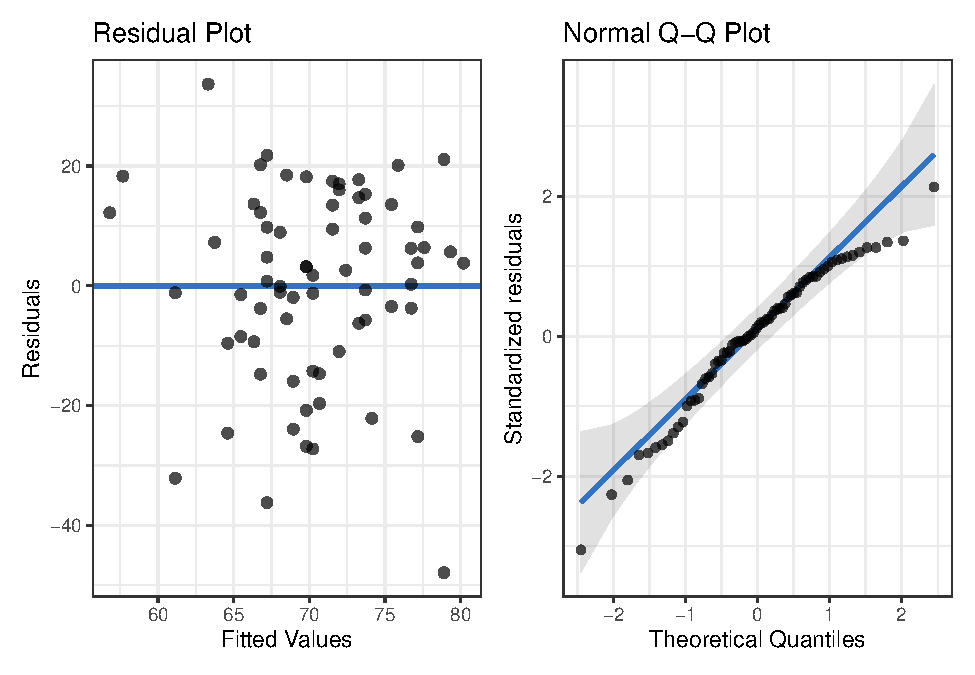
\includegraphics{_main_files/figure-latex/unnamed-chunk-84-1.pdf}

\begin{Shaded}
\begin{Highlighting}[]
\FunctionTok{par}\NormalTok{(}\AttributeTok{mfrow =} \FunctionTok{c}\NormalTok{(}\DecValTok{1}\NormalTok{, }\DecValTok{1}\NormalTok{))}

\FunctionTok{SASreg}\NormalTok{(}\FunctionTok{lm}\NormalTok{(E3 }\SpecialCharTok{\textasciitilde{}}\NormalTok{ Hmwk }\SpecialCharTok{+}\NormalTok{ grp))}
\end{Highlighting}
\end{Shaded}

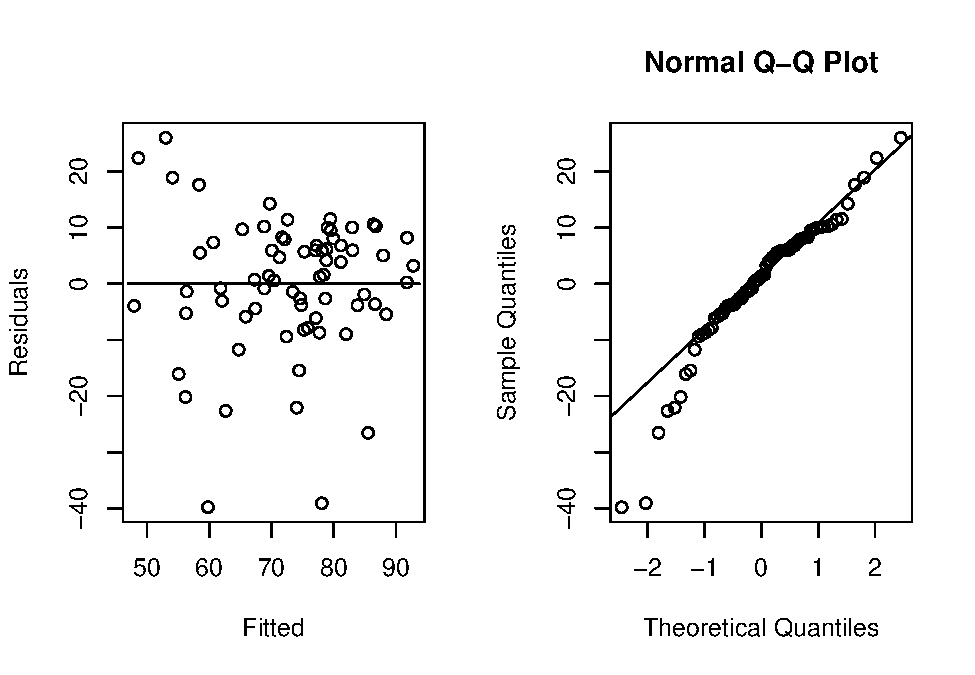
\includegraphics{_main_files/figure-latex/unnamed-chunk-84-2.pdf}

\begin{verbatim}
## $Model.Equation
## 
## Call:
## lm(formula = E3 ~ Hmwk + grp)
## 
## Coefficients:
## (Intercept)         Hmwk       grp1MC       grp1NU       grp1PM       grp2AS  
##    41.28345      0.30491      6.40928      7.61338     15.03430     -0.08199  
##      grp2MC       grp3AS  
##    21.30066     11.37722  
## 
## 
## $Coefficients
## (Intercept)        Hmwk      grp1MC      grp1NU      grp1PM      grp2AS 
## 41.28344540  0.30490745  6.40928451  7.61337963 15.03429656 -0.08198749 
##      grp2MC      grp3AS 
## 21.30066031 11.37722469 
## 
## $Summary
##  Root MSE  R square Adj R-Squ 
##   12.8483    0.4382    0.3748 
## 
## $Analysis.of.Variance
##         Df  Sum Sq Mean Sq F value   Pr(>F)    
## Model    7  7983.1  1140.4  6.9085 4.48e-06 ***
## Error   62 10234.9   165.1                     
## C Total 69 18218.0  5701.6                     
## ---
## Signif. codes:  0 '***' 0.001 '**' 0.01 '*' 0.05 '.' 0.1 ' ' 1
## 
## $Type.I.Tests
##      Df Sum Sq Mean Sq F value    Pr(>F)    
## Hmwk  1 5047.1  5047.1 30.5742 6.834e-07 ***
## grp   6 2936.0   489.3  2.9642    0.0131 *  
## ---
## Signif. codes:  0 '***' 0.001 '**' 0.01 '*' 0.05 '.' 0.1 ' ' 1
## 
## $Type.III.Tests
##      Df Sum Sq F value   Pr(>F)   
## Hmwk  1 1171.5  7.0968 0.009829 **
## grp   6 2936.0  2.9642 0.013097 * 
## ---
## Signif. codes:  0 '***' 0.001 '**' 0.01 '*' 0.05 '.' 0.1 ' ' 1
## 
## $Parameter.Estimates
##             Estimate Std. Error t value Pr(>|t|)    VIF
## (Intercept)  41.2834     8.5089  4.8518   0.0000 0.0000
## Hmwk          0.3049     0.1145  2.6640   0.0098 1.6736
## grp1MC        6.4093     6.0321  1.0625   0.2921 1.0000
## grp1NU        7.6134     6.2702  1.2142   0.2293 1.2937
## grp1PM       15.0343     6.0180  2.4982   0.0151 1.6736
## grp2AS       -0.0820     5.8874 -0.0139   0.9889 6.0000
## grp2MC       21.3007     6.1445  3.4666   0.0010 1.0438
## grp3AS       11.3772     5.8062  1.9595   0.0546 0.0000
\end{verbatim}

Note that the VIFs should not be part of the output in SASreg when categorical variables are present, and this is currently a bug.

Checking whether the lines are parallel can be done simply by checking the interaction Hmwk:grp.

\begin{Shaded}
\begin{Highlighting}[]
\FunctionTok{SASreg}\NormalTok{(}\FunctionTok{lm}\NormalTok{(E3 }\SpecialCharTok{\textasciitilde{}}\NormalTok{ Hmwk }\SpecialCharTok{*}\NormalTok{ grp))}
\end{Highlighting}
\end{Shaded}

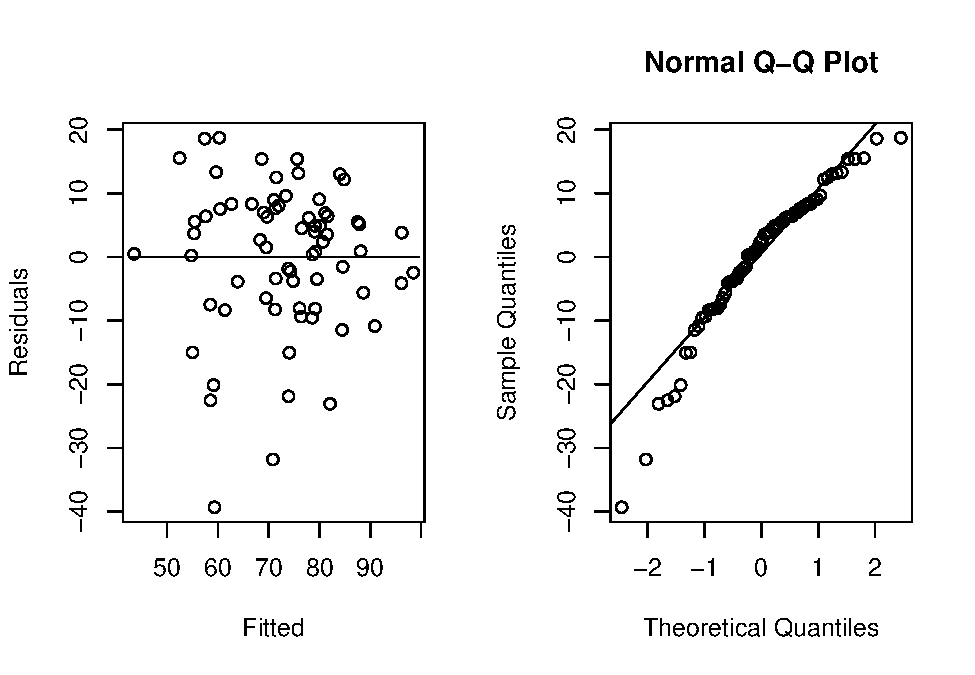
\includegraphics{_main_files/figure-latex/unnamed-chunk-85-1.pdf}

\begin{verbatim}
## $Model.Equation
## 
## Call:
## lm(formula = E3 ~ Hmwk * grp)
## 
## Coefficients:
## (Intercept)         Hmwk       grp1MC       grp1NU       grp1PM       grp2AS  
##    34.65972      0.40631      2.23406      4.29217    -39.95759     32.07351  
##      grp2MC       grp3AS  Hmwk:grp1MC  Hmwk:grp1NU  Hmwk:grp1PM  Hmwk:grp2AS  
##    -4.41607     13.08221      0.03133      0.01258      0.65975     -0.57325  
## Hmwk:grp2MC  Hmwk:grp3AS  
##     0.28205     -0.03366  
## 
## 
## $Coefficients
##  (Intercept)         Hmwk       grp1MC       grp1NU       grp1PM       grp2AS 
##  34.65972374   0.40631164   2.23406485   4.29216905 -39.95759295  32.07351063 
##       grp2MC       grp3AS  Hmwk:grp1MC  Hmwk:grp1NU  Hmwk:grp1PM  Hmwk:grp2AS 
##  -4.41607393  13.08221050   0.03132616   0.01257784   0.65975222  -0.57325369 
##  Hmwk:grp2MC  Hmwk:grp3AS 
##   0.28204916  -0.03366234 
## 
## $Summary
##  Root MSE  R square Adj R-Squ 
##   12.7778    0.4981    0.3816 
## 
## $Analysis.of.Variance
##         Df  Sum Sq Mean Sq F value    Pr(>F)    
## Model   13  9074.8   698.1  4.2754 6.298e-05 ***
## Error   56  9143.2   163.3                      
## C Total 69 18218.0  5881.7                      
## ---
## Signif. codes:  0 '***' 0.001 '**' 0.01 '*' 0.05 '.' 0.1 ' ' 1
## 
## $Type.I.Tests
##          Df Sum Sq Mean Sq F value   Pr(>F)    
## Hmwk      1 5047.1  5047.1 30.9125 7.81e-07 ***
## grp       6 2936.0   489.3  2.9970  0.01306 *  
## Hmwk:grp  6 1091.6   181.9  1.1143  0.36580    
## ---
## Signif. codes:  0 '***' 0.001 '**' 0.01 '*' 0.05 '.' 0.1 ' ' 1
## 
## $Type.III.Tests
##          Df  Sum Sq F value  Pr(>F)  
## Hmwk      1  690.67  4.2302 0.04438 *
## grp       6  714.43  0.7293 0.62795  
## Hmwk:grp  6 1091.64  1.1143 0.36580  
## ---
## Signif. codes:  0 '***' 0.001 '**' 0.01 '*' 0.05 '.' 0.1 ' ' 1
## 
## $Parameter.Estimates
##             Estimate Std. Error t value Pr(>|t|)          VIF
## (Intercept)  34.6597    13.5219  2.5632   0.0131 0.000000e+00
## Hmwk          0.4063     0.1976  2.0567   0.0444 5.041000e+00
## grp1MC        2.2341    30.5272  0.0732   0.9419 1.000000e+00
## grp1NU        4.2922    43.3093  0.0991   0.9214 2.245200e+00
## grp1PM      -39.9576    55.3296 -0.7222   0.4732 9.571270e+09
## grp2AS       32.0735    18.9058  1.6965   0.0953 6.000000e+00
## grp2MC       -4.4161    41.0984 -0.1075   0.9148 6.788100e+00
## grp3AS       13.0822    24.9749  0.5238   0.6025 1.132895e+10
## Hmwk:grp1MC   0.0313     0.3869  0.0810   0.9358 6.000000e+00
## Hmwk:grp1NU   0.0126     0.5092  0.0247   0.9804 6.884100e+00
## Hmwk:grp1PM   0.6598     0.6898  0.9565   0.3430 0.000000e+00
## Hmwk:grp2AS  -0.5733     0.3051 -1.8790   0.0655 5.041000e+00
## Hmwk:grp2MC   0.2820     0.4985  0.5658   0.5738 1.000000e+00
## Hmwk:grp3AS  -0.0337     0.3458 -0.0974   0.9228 2.245200e+00
\end{verbatim}

\hypertarget{other-methods}{%
\section{Other Methods}\label{other-methods}}

Functions in base SAS for other commonly used methods include:

For Nonparametrics:

\begin{itemize}
\tightlist
\item
  \texttt{wilcox.test()}
\item
  \texttt{friedman.test()}
\item
  \texttt{kruskal.test()}
\end{itemize}

For Categorical Data:

\begin{itemize}
\tightlist
\item
  \texttt{binom.test()}
\item
  \texttt{chisq.test()}
\item
  \texttt{glm(\ ,family=binomial("logit"))}
\item
  \texttt{fisher.test()}
\item
  \texttt{mantel.haen.test()}
\end{itemize}

\hypertarget{manipulating-data}{%
\chapter{Manipulating Data}\label{manipulating-data}}

\hypertarget{dplyr-basics}{%
\section*{dplyr basics}\label{dplyr-basics}}
\addcontentsline{toc}{section}{dplyr basics}

\hypertarget{filter-rows}{%
\section{Filter rows}\label{filter-rows}}

\begin{itemize}
\tightlist
\item
  Comparisons
\item
  Logical operators
\item
  Missing values
\end{itemize}

\hypertarget{arrange-rows}{%
\section{Arrange rows}\label{arrange-rows}}

\hypertarget{select-columns}{%
\section{Select columns}\label{select-columns}}

\hypertarget{add-new-variables}{%
\section{Add new variables}\label{add-new-variables}}

\hypertarget{grouped-summaries}{%
\section{Grouped summaries}\label{grouped-summaries}}

\begin{itemize}
\tightlist
\item
  Combining multiple operations with the pipe
\item
  Missing values
\item
  Counts
\item
  Useful summary functions
\item
  Grouping by multiple variables
\item
  Ungrouping
\end{itemize}

\hypertarget{grouped-mutates-and-filters}{%
\section{Grouped mutates (and filters)}\label{grouped-mutates-and-filters}}

\hypertarget{an-example}{%
\section{An example}\label{an-example}}

The following example ties several of the above ideas together. Imagine that we have a set of grades from a course that we would like to convert to letter grades using a particular weighting and letter-grade cut-offs.

\begin{Shaded}
\begin{Highlighting}[]
\NormalTok{students }\OtherTok{\textless{}{-}}\NormalTok{ readr}\SpecialCharTok{::}\FunctionTok{read\_table}\NormalTok{(}\StringTok{"data/CourseData.txt"}\NormalTok{)[, }\SpecialCharTok{{-}}\DecValTok{1}\NormalTok{]}
\FunctionTok{head}\NormalTok{(students)}
\end{Highlighting}
\end{Shaded}

\begin{verbatim}
## # A tibble: 6 x 6
##   College  Year  Hmwk    E1    E2    E3
##   <chr>   <dbl> <dbl> <dbl> <dbl> <dbl>
## 1 NU          1  83.8    79    89    59
## 2 NU          1  77.1    60    97    63
## 3 NU          1  94.5    83    88    69
## 4 NU          1  84.3    91    77    72
## 5 NU          1  73.4    68    79    76
## 6 NU          1  94.7    89    96    79
\end{verbatim}

\begin{Shaded}
\begin{Highlighting}[]
\FunctionTok{tail}\NormalTok{(students)}
\end{Highlighting}
\end{Shaded}

\begin{verbatim}
## # A tibble: 6 x 6
##   College  Year  Hmwk    E1    E2    E3
##   <chr>   <dbl> <dbl> <dbl> <dbl> <dbl>
## 1 MC          2  83.2    69    77    93
## 2 MC          2  95.7    88    89    92
## 3 MC          2  79.3    80    61    97
## 4 MC          2  78.1    69    89    97
## 5 MC          2  99.1    84    89    96
## 6 MC          2  95.8    96   100   100
\end{verbatim}

In this particular case we want the weighting to be:

\begin{itemize}
\tightlist
\item
  20\% to Hmwk (col 3)
\item
  25\% to E1 (col 4)
\item
  25\% to E2 (col 5)
\item
  30\% to E3 (col 6)
\end{itemize}

But those weights could change later. A function can be written to take the data, and the weights and calculate the weighted average. We can then add that score to the students data frame, and add a final column with the actual letter grades on a 90-80-70-60 scale.

\begin{Shaded}
\begin{Highlighting}[]
\NormalTok{students }\OtherTok{\textless{}{-}}\NormalTok{ students }\SpecialCharTok{\%\textgreater{}\%} 
  \FunctionTok{mutate}\NormalTok{(}\AttributeTok{Final =}\NormalTok{ .}\DecValTok{2}\SpecialCharTok{*}\NormalTok{Hmwk }\SpecialCharTok{+}\NormalTok{ .}\DecValTok{25}\SpecialCharTok{*}\NormalTok{E1 }\SpecialCharTok{+}\NormalTok{ .}\DecValTok{25}\SpecialCharTok{*}\NormalTok{E2 }\SpecialCharTok{+}\NormalTok{ .}\DecValTok{3}\SpecialCharTok{*}\NormalTok{E3,}
         \AttributeTok{Grade =} \FunctionTok{case\_when}\NormalTok{(}
\NormalTok{           Final }\SpecialCharTok{\textless{}} \DecValTok{60} \SpecialCharTok{\textasciitilde{}} \StringTok{"F"}\NormalTok{,}
\NormalTok{           Final }\SpecialCharTok{\textless{}} \DecValTok{69} \SpecialCharTok{\textasciitilde{}} \StringTok{"D"}\NormalTok{,}
\NormalTok{           Final }\SpecialCharTok{\textless{}} \DecValTok{79} \SpecialCharTok{\textasciitilde{}} \StringTok{"C"}\NormalTok{,}
\NormalTok{           Final }\SpecialCharTok{\textless{}} \DecValTok{89} \SpecialCharTok{\textasciitilde{}} \StringTok{"B"}\NormalTok{,}
\NormalTok{           Final }\SpecialCharTok{\textgreater{}=} \DecValTok{90} \SpecialCharTok{\textasciitilde{}} \StringTok{"A"}\NormalTok{))}

\FunctionTok{head}\NormalTok{(students)}
\end{Highlighting}
\end{Shaded}

\begin{verbatim}
## # A tibble: 6 x 8
##   College  Year  Hmwk    E1    E2    E3 Final Grade
##   <chr>   <dbl> <dbl> <dbl> <dbl> <dbl> <dbl> <chr>
## 1 NU          1  83.8    79    89    59  76.5 C    
## 2 NU          1  77.1    60    97    63  73.6 C    
## 3 NU          1  94.5    83    88    69  82.4 B    
## 4 NU          1  84.3    91    77    72  80.5 B    
## 5 NU          1  73.4    68    79    76  74.2 C    
## 6 NU          1  94.7    89    96    79  88.9 B
\end{verbatim}

\hypertarget{extra-working-with-factor-variables}{%
\section{Extra: Working with factor variables}\label{extra-working-with-factor-variables}}

\hypertarget{graphics}{%
\chapter{Graphics}\label{graphics}}

\hypertarget{outline}{%
\section*{Outline}\label{outline}}
\addcontentsline{toc}{section}{Outline}

\hypertarget{introduction-to-ggplot2}{%
\paragraph*{1. Introduction to ggplot2}\label{introduction-to-ggplot2}}
\addcontentsline{toc}{paragraph}{1. Introduction to ggplot2}

\begin{itemize}
\tightlist
\item
  setup
\item
  why ggplot2
\item
  the evolution of a ggplot
\item
  create your first ggplot
\end{itemize}

\hypertarget{ggplot2-concepts}{%
\paragraph*{2. ggplot2 concepts}\label{ggplot2-concepts}}
\addcontentsline{toc}{paragraph}{2. ggplot2 concepts}

\begin{itemize}
\tightlist
\item
  the grammar of ggplot2
\item
  geometrical layers
\item
  statistical layers
\item
  facets
\item
  ggplots as objects
\end{itemize}

\hypertarget{advanced-customization}{%
\paragraph*{3. Advanced customization}\label{advanced-customization}}
\addcontentsline{toc}{paragraph}{3. Advanced customization}

\begin{itemize}
\tightlist
\item
  scales
\item
  coordinates
\item
  labels
\item
  annotations
\item
  themes
\item
  legends
\item
  fonts
\end{itemize}

\hypertarget{extensions}{%
\paragraph*{4. Extensions}\label{extensions}}
\addcontentsline{toc}{paragraph}{4. Extensions}

\begin{itemize}
\tightlist
\item
  patchwork
\item
  gganimate
\item
  ggplotly
\item
  ggiraph
\end{itemize}

\hypertarget{introduction}{%
\section{Introduction}\label{introduction}}

\begin{itemize}
\tightlist
\item
  setup
\item
  intro to ggplot2
\item
  why ggplot2
\item
  showcase (glimpse)
\item
  the evolution of a ggplot
\item
  showcase in detail?
\item
  create your first ggplot
\end{itemize}

\hypertarget{ggplot2-concepts-1}{%
\section{ggplot2 concepts}\label{ggplot2-concepts-1}}

\begin{itemize}
\tightlist
\item
  the grammar of ggplot2
\item
  walk through example

  \begin{itemize}
  \tightlist
  \item
    aesthetic mapping
  \end{itemize}
\item
  geometrical layers

  \begin{itemize}
  \tightlist
  \item
    geoms
  \item
    Setting vs Mapping of Visual Properties
  \item
    Local vs.~Global Encoding
  \item
    Adding More Layers
  \item
    The \texttt{group} Aesthetic
  \item
    Overwrite Global Aesthetics
  \end{itemize}
\item
  statistical layers

  \begin{itemize}
  \tightlist
  \item
    \texttt{stat\_*()} and \texttt{geom\_*()}
  \item
    statistical summaries
  \end{itemize}
\item
  facets
\item
  Store a ggplot as Object

  \begin{itemize}
  \tightlist
  \item
    inspect a ggplot Object
  \item
    extend a ggplot Object
  \end{itemize}
\end{itemize}

\hypertarget{advanced-customization-1}{%
\section{Advanced customization}\label{advanced-customization-1}}

\begin{itemize}
\tightlist
\item
  scales

  \begin{itemize}
  \tightlist
  \item
    continuous vs.~discrete
  \item
    aesthetics + scales
  \end{itemize}
\item
  coordinates
\item
  labels
\item
  annotations
\item
  themes
\item
  legends
\item
  fonts
\end{itemize}

\hypertarget{extensions-1}{%
\section{Extensions}\label{extensions-1}}

\begin{itemize}
\tightlist
\item
  ggplot2 extensions
\item
  gganimate
\item
  ggplotly
\item
  ggiraph
\end{itemize}

\hypertarget{psychometric-packages}{%
\chapter{Psychometric Packages}\label{psychometric-packages}}

There are a number of packages that can be used for psychometric analysis. The following code uses a small sample of what is out there. A good reference with a list of numerous packages can be found at \url{https://cran.r-project.org/web/views/Psychometrics.html}. This section contains some examples from the \textbf{CTT}, \textbf{psychometric}, \textbf{psych}, \textbf{difr}, and \textbf{mirt} packages.

The first several examples use the data set \texttt{samptest.txt}. It also gives a chance to see how to score an exam using the \emph{CTT} package. The next lines enter the answer key, format it for later use, and read in the data set.

\begin{Shaded}
\begin{Highlighting}[]
\DocumentationTok{\#\# sample test data with 36 items and 2 demographic variables (ethnicity and gender)}
\NormalTok{key }\OtherTok{\textless{}{-}} \StringTok{"ADCABCACDCDCBBCBDCADADCABDBABADBCADB"}
\NormalTok{new.key }\OtherTok{\textless{}{-}} \FunctionTok{unlist}\NormalTok{(}\FunctionTok{strsplit}\NormalTok{(key, }\AttributeTok{split =} \StringTok{""}\NormalTok{))}
\NormalTok{testdat }\OtherTok{\textless{}{-}} \FunctionTok{read.fwf}\NormalTok{(}\StringTok{"data/samptest.txt"}\NormalTok{, }\AttributeTok{widths =} \FunctionTok{c}\NormalTok{(}\FunctionTok{rep}\NormalTok{(}\DecValTok{1}\NormalTok{, }\DecValTok{38}\NormalTok{)))}
\FunctionTok{dim}\NormalTok{(testdat)}
\end{Highlighting}
\end{Shaded}

\begin{verbatim}
## [1] 102  38
\end{verbatim}

\begin{Shaded}
\begin{Highlighting}[]
\FunctionTok{head}\NormalTok{(testdat)}
\end{Highlighting}
\end{Shaded}

\begin{verbatim}
##   V1 V2 V3 V4 V5 V6 V7 V8 V9 V10 V11 V12 V13 V14 V15 V16 V17 V18 V19 V20 V21
## 1  A  D  A  A  B  C  A  C  C   C   D   C   C   D   D   B   D   C   B   D   A
## 2  A  D  C  A  B  C  A  C  D   C   D   C   B   B   C   B   D   C   A   D   A
## 3  C  C  D  A  B  B  A  C  C   D   C   C   B   D   A   B   D   C   A   D   A
## 4  A  D  B  A  B  C  A  C  D   C   D   C   B   B   C   A   D   C   A   D   A
## 5  A  D  C  A  B  C  A  A  D   C   D   C   B   B   C   B   D   C   A   D   A
## 6  A  B  A  A  B  C  A  C  A   C   C   C   B   B   D   B   D   C   A   D   B
##   V22 V23 V24 V25 V26 V27 V28 V29 V30 V31 V32 V33 V34 V35 V36 V37 V38
## 1   D   A   A   B   D   B   A   B   A   D   B   C   A   D   B   B   F
## 2   D   C   A   B   D   B   A   B   A   D   B   C   A   D   B   W   F
## 3   A   A   A   B   A   D   A   B   A   B   B   A   A   A   D   B   F
## 4   D   C   A   B   D   B   A   B   A   D   B   C   A   B   B   B   M
## 5   B   C   A   B   D   B   A   B   A   D   B   C   A   D   B   B   F
## 6   D   A   A   B   D   C   A   B   C   D   B   C   D   B   B   B   M
\end{verbatim}

The \textbf{CTT} package contains basic data functions like \texttt{distractorAnalysis()}, and \texttt{score()} for scoring the data.

\begin{Shaded}
\begin{Highlighting}[]
\FunctionTok{library}\NormalTok{(CTT)}
\FunctionTok{distractorAnalysis}\NormalTok{(testdat[, }\DecValTok{1}\SpecialCharTok{:}\DecValTok{36}\NormalTok{], }\AttributeTok{key =}\NormalTok{ new.key)[[}\DecValTok{1}\NormalTok{]]}
\end{Highlighting}
\end{Shaded}

\begin{verbatim}
##   correct key  n       rspP       pBis    discrim     lower     mid50     mid75
## A       *   A 75 0.73529412  0.5149574  0.5806452 0.4193548 0.8571429 0.7692308
## B           B  7 0.06862745 -0.5289839 -0.2258065 0.2258065 0.0000000 0.0000000
## C           C 11 0.10784314 -0.2247585 -0.1612903 0.1612903 0.1428571 0.1153846
## D           D  9 0.08823529 -0.2920536 -0.1935484 0.1935484 0.0000000 0.1153846
## P           P  0 0.00000000         NA  0.0000000 0.0000000 0.0000000 0.0000000
##   upper
## A     1
## B     0
## C     0
## D     0
## P     0
\end{verbatim}

\begin{Shaded}
\begin{Highlighting}[]
\CommentTok{\# score gives both the sum scores and the response matrix}
\NormalTok{scoredat }\OtherTok{\textless{}{-}} \FunctionTok{score}\NormalTok{(testdat[, }\DecValTok{1}\SpecialCharTok{:}\DecValTok{36}\NormalTok{], new.key, }\AttributeTok{output.scored =} \ConstantTok{TRUE}\NormalTok{)}

\CommentTok{\# get 0/1 responses only}
\NormalTok{responses }\OtherTok{\textless{}{-}}\NormalTok{ scoredat}\SpecialCharTok{$}\NormalTok{scored}

\CommentTok{\# get the total scores only}
\NormalTok{sumscores }\OtherTok{\textless{}{-}}\NormalTok{ scoredat}\SpecialCharTok{$}\NormalTok{score}
\end{Highlighting}
\end{Shaded}

It also includes some basic classical analyses:

\begin{Shaded}
\begin{Highlighting}[]
\FunctionTok{itemAnalysis}\NormalTok{(responses)}
\end{Highlighting}
\end{Shaded}

\begin{verbatim}
## 
##  Number of Items 
##  36 
## 
##  Number of Examinees 
##  102 
## 
##  Coefficient Alpha 
##  0.844
\end{verbatim}

The \textbf{psychometric} and \textbf{psych} packages overlap some, but are both larger.

\begin{Shaded}
\begin{Highlighting}[]
\FunctionTok{library}\NormalTok{(psychometric)}
\FunctionTok{alpha}\NormalTok{(responses)}
\end{Highlighting}
\end{Shaded}

\begin{verbatim}
## [1] 0.8441692
\end{verbatim}

\begin{Shaded}
\begin{Highlighting}[]
\FunctionTok{alpha.CI}\NormalTok{(}\FunctionTok{alpha}\NormalTok{(responses), }\AttributeTok{N =} \FunctionTok{dim}\NormalTok{(responses)[}\DecValTok{1}\NormalTok{], }\AttributeTok{k =} \FunctionTok{dim}\NormalTok{(responses)[}\DecValTok{2}\NormalTok{])}
\end{Highlighting}
\end{Shaded}

\begin{verbatim}
##         LCL     ALPHA       UCL
## 1 0.8057113 0.8441692 0.8787447
\end{verbatim}

\begin{Shaded}
\begin{Highlighting}[]
\FunctionTok{library}\NormalTok{(psych)}
\NormalTok{psych}\SpecialCharTok{::}\FunctionTok{polyserial}\NormalTok{(}\FunctionTok{as.matrix}\NormalTok{(sumscores), }\FunctionTok{as.matrix}\NormalTok{(responses[, }\DecValTok{1}\NormalTok{]))}
\end{Highlighting}
\end{Shaded}

\begin{verbatim}
##           [,1]
## [1,] 0.7657925
\end{verbatim}

It is important to check that the functions in each package actually do what you want. In the case of measuring item discrimination using the biserial correlation of the items with the rest score, it's necessary to check that the polyserial funcion in the psych package is the one you want to agree with texts like Lord and Novick, or Crocker and Algina.

\begin{Shaded}
\begin{Highlighting}[]
\NormalTok{biserials }\OtherTok{\textless{}{-}} \ConstantTok{NULL}
\ControlFlowTok{for}\NormalTok{ (i }\ControlFlowTok{in} \DecValTok{1}\SpecialCharTok{:}\FunctionTok{ncol}\NormalTok{(responses)) \{}
\NormalTok{  biserials }\OtherTok{\textless{}{-}} \FunctionTok{c}\NormalTok{(biserials, }\FunctionTok{polyserial}\NormalTok{(}\FunctionTok{as.matrix}\NormalTok{(sumscores }\SpecialCharTok{{-}}\NormalTok{ responses[, i]), }\FunctionTok{as.matrix}\NormalTok{(responses[, i])))}
\NormalTok{\}}
\NormalTok{biserials}
\end{Highlighting}
\end{Shaded}

\begin{verbatim}
##  [1] 0.69400052 0.50200231 0.30618509 0.45158311 0.38036029 0.51107140
##  [7] 0.26724319 0.37702310 0.58276455 0.68733895 0.55842935 0.70796675
## [13] 0.30582385 0.08002487 0.46911103 0.11720900 0.64378754 0.46670904
## [19] 0.26342658 0.70517564 0.50782867 0.59232271 0.41577996 0.57712603
## [25] 0.52496694 0.52036168 0.47193436 0.27588499 0.25170829 0.40882539
## [31] 0.40607968 0.67815832 0.47517826 0.52294511 0.42049977 0.55669711
\end{verbatim}

Among the more specialized packages are those that do more specialized procedures such as DIF detection in the difR package.

\begin{Shaded}
\begin{Highlighting}[]
\CommentTok{\# Looking at difR}
\FunctionTok{library}\NormalTok{(difR)}
\NormalTok{difdat }\OtherTok{\textless{}{-}} \FunctionTok{data.frame}\NormalTok{(responses, testdat[, }\DecValTok{38}\NormalTok{])}
\FunctionTok{dichoDif}\NormalTok{(difdat, }\AttributeTok{group =} \DecValTok{37}\NormalTok{, }\AttributeTok{focal.name =} \StringTok{"F"}\NormalTok{, }\AttributeTok{method =} \FunctionTok{c}\NormalTok{(}\StringTok{"MH"}\NormalTok{, }\StringTok{"Logistic"}\NormalTok{), }\AttributeTok{criterion =} \StringTok{"Wald"}\NormalTok{)}
\end{Highlighting}
\end{Shaded}

\begin{verbatim}
## Comparison of DIF detection results using 2 methods 
##  
## Methods used: 
##  Mantel-Haenszel
##  Logistic regression
## 
## Matching variable: test score 
##  
## No set of anchor items was provided 
##  
## Parameters: 
##  Significance level: 0.05
##  Mantel-Haenszel DIF statistic: Chi-square statistic 
##  Mantel-Haenszel continuity correction: Yes 
##  Type of Mantel-Haenszel test: asymptotic test 
##  Logistic regression DIF statistic: Wald statistic 
##  DIF effect(s) tested by logistic regression: both DIF effects 
##  Item purification: No 
##  
##  No p-value adjustment for multiple comparisons 
##  
## Comparison of DIF detection results: 
##  
##     M-H   Logistic #DIF 
## V1   DIF  NoDIF     1/2 
## V2  NoDIF  DIF      1/2 
## V3  NoDIF NoDIF     0/2 
## V4   DIF  NoDIF     1/2 
## V5  NoDIF NoDIF     0/2 
## V6  NoDIF NoDIF     0/2 
## V7  NoDIF NoDIF     0/2 
## V8  NoDIF NoDIF     0/2 
## V9   DIF  NoDIF     1/2 
## V10 NoDIF  DIF      1/2 
## V11 NoDIF NoDIF     0/2 
## V12 NoDIF NoDIF     0/2 
## V13 NoDIF NoDIF     0/2 
## V14 NoDIF NoDIF     0/2 
## V15 NoDIF NoDIF     0/2 
## V16 NoDIF NoDIF     0/2 
## V17 NoDIF NoDIF     0/2 
## V18 NoDIF NoDIF     0/2 
## V19 NoDIF NoDIF     0/2 
## V20 NoDIF NoDIF     0/2 
## V21 NoDIF  DIF      1/2 
## V22 NoDIF NoDIF     0/2 
## V23 NoDIF NoDIF     0/2 
## V24 NoDIF NoDIF     0/2 
## V25 NoDIF NoDIF     0/2 
## V26 NoDIF NoDIF     0/2 
## V27 NoDIF NoDIF     0/2 
## V28 NoDIF NoDIF     0/2 
## V29 NoDIF  DIF      1/2 
## V30 NoDIF NoDIF     0/2 
## V31 NoDIF NoDIF     0/2 
## V32 NoDIF  DIF      1/2 
## V33 NoDIF NoDIF     0/2 
## V34 NoDIF NoDIF     0/2 
## V35 NoDIF NoDIF     0/2 
## V36 NoDIF NoDIF     0/2 
## 
##  Output was not captured!
\end{verbatim}

There are also packages for estimating IRT models, icluding the mirt package. A larger data set is used for this example.

\begin{Shaded}
\begin{Highlighting}[]
\NormalTok{mdatab2 }\OtherTok{\textless{}{-}} \FunctionTok{read.fwf}\NormalTok{(}\StringTok{"data/mdatab.txt"}\NormalTok{, }\AttributeTok{widths =} \FunctionTok{rep}\NormalTok{(}\DecValTok{1}\NormalTok{, }\DecValTok{32}\NormalTok{))}
\FunctionTok{dim}\NormalTok{(mdatab2)}
\end{Highlighting}
\end{Shaded}

\begin{verbatim}
## [1] 2642   32
\end{verbatim}

\begin{Shaded}
\begin{Highlighting}[]
\FunctionTok{head}\NormalTok{(mdatab2)}
\end{Highlighting}
\end{Shaded}

\begin{verbatim}
##   V1 V2 V3 V4 V5 V6 V7 V8 V9 V10 V11 V12 V13 V14 V15 V16 V17 V18 V19 V20 V21
## 1  1  1  0  1  1  1  1  1  1   1   0   0   0   1   1   0   0   0   0   0   0
## 2  1  1  1  1  1  1  0  0  1   1   0   0   0   0   0   0   1   0   1   0   0
## 3  0  0  0  0  1  0  1  1  1   1   0   0   0   0   0   0   0   0   0   0   0
## 4  1  1  1  1  0  1  0  1  0   0   0   1   0   1   1   0   0   1   1   1   0
## 5  1  0  0  0  0  0  0  0  1   0   0   0   0   0   1   0   0   1   0   1   0
## 6  1  1  1  1  1  1  1  0  0   0   1   0   0   0   0   0   1   0   0   1   0
##   V22 V23 V24 V25 V26 V27 V28 V29 V30 V31 V32
## 1   0   1   1   1   0   0   0   0   0   1   0
## 2   0   1   0   0   0   1   0   0   0   0   0
## 3   0   0   0   1   0   0   0   1   0   0   0
## 4   0   0   1   0   0   0   0   0   1   1   0
## 5   0   0   0   0   0   1   0   1   0   0   0
## 6   0   0   0   1   0   0   0   0   0   0   0
\end{verbatim}

\begin{Shaded}
\begin{Highlighting}[]
\CommentTok{\# mirt package}
\FunctionTok{library}\NormalTok{(mirt)}

\CommentTok{\# estimating IRT model parameters}
\NormalTok{mod1.rasch }\OtherTok{\textless{}{-}} \FunctionTok{mirt}\NormalTok{(mdatab2, }\DecValTok{1}\NormalTok{, }\AttributeTok{itemtype =} \StringTok{"Rasch"}\NormalTok{)}
\end{Highlighting}
\end{Shaded}

\begin{verbatim}
## Iteration: 1, Log-Lik: -50361.109, Max-Change: 0.09008Iteration: 2, Log-Lik: -50349.088, Max-Change: 0.03676Iteration: 3, Log-Lik: -50347.375, Max-Change: 0.01433Iteration: 4, Log-Lik: -50347.103, Max-Change: 0.00558Iteration: 5, Log-Lik: -50347.049, Max-Change: 0.00245Iteration: 6, Log-Lik: -50347.040, Max-Change: 0.00100Iteration: 7, Log-Lik: -50347.037, Max-Change: 0.00040Iteration: 8, Log-Lik: -50347.037, Max-Change: 0.00020Iteration: 9, Log-Lik: -50347.036, Max-Change: 0.00015Iteration: 10, Log-Lik: -50347.035, Max-Change: 0.00007
\end{verbatim}

\begin{Shaded}
\begin{Highlighting}[]
\NormalTok{mod1}\FloatTok{.3}\NormalTok{PL }\OtherTok{\textless{}{-}} \FunctionTok{mirt}\NormalTok{(mdatab2, }\DecValTok{1}\NormalTok{, }\AttributeTok{itemtype =} \StringTok{"3PL"}\NormalTok{)}
\end{Highlighting}
\end{Shaded}

\begin{verbatim}
## Iteration: 1, Log-Lik: -50725.510, Max-Change: 3.35905Iteration: 2, Log-Lik: -50127.462, Max-Change: 1.09803Iteration: 3, Log-Lik: -49965.395, Max-Change: 0.55587Iteration: 4, Log-Lik: -49895.478, Max-Change: 0.46573Iteration: 5, Log-Lik: -49854.195, Max-Change: 0.39404Iteration: 6, Log-Lik: -49829.228, Max-Change: 0.26644Iteration: 7, Log-Lik: -49813.057, Max-Change: 0.44325Iteration: 8, Log-Lik: -49802.681, Max-Change: 0.38998Iteration: 9, Log-Lik: -49796.321, Max-Change: 0.23153Iteration: 10, Log-Lik: -49791.428, Max-Change: 0.71392Iteration: 11, Log-Lik: -49787.926, Max-Change: 0.17278Iteration: 12, Log-Lik: -49785.424, Max-Change: 0.09802Iteration: 13, Log-Lik: -49783.996, Max-Change: 0.14081Iteration: 14, Log-Lik: -49782.271, Max-Change: 0.06688Iteration: 15, Log-Lik: -49781.061, Max-Change: 0.12363Iteration: 16, Log-Lik: -49779.781, Max-Change: 0.08094Iteration: 17, Log-Lik: -49779.219, Max-Change: 0.39285Iteration: 18, Log-Lik: -49778.536, Max-Change: 0.53760Iteration: 19, Log-Lik: -49788.762, Max-Change: 0.20207Iteration: 20, Log-Lik: -49777.043, Max-Change: 0.05616Iteration: 21, Log-Lik: -49776.879, Max-Change: 0.00634Iteration: 22, Log-Lik: -49776.873, Max-Change: 0.00614Iteration: 23, Log-Lik: -49776.830, Max-Change: 0.00240Iteration: 24, Log-Lik: -49776.801, Max-Change: 0.00252Iteration: 25, Log-Lik: -49776.722, Max-Change: 0.00453Iteration: 26, Log-Lik: -49776.718, Max-Change: 0.00139Iteration: 27, Log-Lik: -49776.713, Max-Change: 0.00113Iteration: 28, Log-Lik: -49776.708, Max-Change: 0.00137Iteration: 29, Log-Lik: -49776.706, Max-Change: 0.00053Iteration: 30, Log-Lik: -49776.705, Max-Change: 0.00023Iteration: 31, Log-Lik: -49776.704, Max-Change: 0.00023Iteration: 32, Log-Lik: -49776.703, Max-Change: 0.00022Iteration: 33, Log-Lik: -49776.703, Max-Change: 0.00021Iteration: 34, Log-Lik: -49776.701, Max-Change: 0.00078Iteration: 35, Log-Lik: -49776.701, Max-Change: 0.00062Iteration: 36, Log-Lik: -49776.700, Max-Change: 0.00053Iteration: 37, Log-Lik: -49776.699, Max-Change: 0.00036Iteration: 38, Log-Lik: -49776.699, Max-Change: 0.00035Iteration: 39, Log-Lik: -49776.699, Max-Change: 0.00017Iteration: 40, Log-Lik: -49776.699, Max-Change: 0.00067Iteration: 41, Log-Lik: -49776.699, Max-Change: 0.00039Iteration: 42, Log-Lik: -49776.698, Max-Change: 0.00034Iteration: 43, Log-Lik: -49776.698, Max-Change: 0.00030Iteration: 44, Log-Lik: -49776.698, Max-Change: 0.00034Iteration: 45, Log-Lik: -49776.698, Max-Change: 0.00015Iteration: 46, Log-Lik: -49776.698, Max-Change: 0.00011Iteration: 47, Log-Lik: -49776.698, Max-Change: 0.00030Iteration: 48, Log-Lik: -49776.698, Max-Change: 0.00034Iteration: 49, Log-Lik: -49776.698, Max-Change: 0.00019Iteration: 50, Log-Lik: -49776.697, Max-Change: 0.00030Iteration: 51, Log-Lik: -49776.697, Max-Change: 0.00013Iteration: 52, Log-Lik: -49776.697, Max-Change: 0.00011Iteration: 53, Log-Lik: -49776.697, Max-Change: 0.00028Iteration: 54, Log-Lik: -49776.697, Max-Change: 0.00037Iteration: 55, Log-Lik: -49776.697, Max-Change: 0.00019Iteration: 56, Log-Lik: -49776.697, Max-Change: 0.00028Iteration: 57, Log-Lik: -49776.697, Max-Change: 0.00012Iteration: 58, Log-Lik: -49776.697, Max-Change: 0.00010
\end{verbatim}

\begin{Shaded}
\begin{Highlighting}[]
\FunctionTok{coef}\NormalTok{(mod1.rasch)}
\end{Highlighting}
\end{Shaded}

\begin{verbatim}
## $V1
##     a1     d g u
## par  1 0.462 0 1
## 
## $V2
##     a1     d g u
## par  1 1.137 0 1
## 
## $V3
##     a1     d g u
## par  1 0.797 0 1
## 
## $V4
##     a1     d g u
## par  1 1.077 0 1
## 
## $V5
##     a1     d g u
## par  1 1.827 0 1
## 
## $V6
##     a1     d g u
## par  1 1.032 0 1
## 
## $V7
##     a1     d g u
## par  1 -0.51 0 1
## 
## $V8
##     a1     d g u
## par  1 0.482 0 1
## 
## $V9
##     a1     d g u
## par  1 0.801 0 1
## 
## $V10
##     a1     d g u
## par  1 0.575 0 1
## 
## $V11
##     a1      d g u
## par  1 -0.262 0 1
## 
## $V12
##     a1     d g u
## par  1 1.275 0 1
## 
## $V13
##     a1      d g u
## par  1 -1.241 0 1
## 
## $V14
##     a1     d g u
## par  1 1.232 0 1
## 
## $V15
##     a1     d g u
## par  1 0.045 0 1
## 
## $V16
##     a1      d g u
## par  1 -0.624 0 1
## 
## $V17
##     a1     d g u
## par  1 0.251 0 1
## 
## $V18
##     a1     d g u
## par  1 0.154 0 1
## 
## $V19
##     a1     d g u
## par  1 0.733 0 1
## 
## $V20
##     a1      d g u
## par  1 -0.021 0 1
## 
## $V21
##     a1      d g u
## par  1 -0.342 0 1
## 
## $V22
##     a1      d g u
## par  1 -0.473 0 1
## 
## $V23
##     a1      d g u
## par  1 -0.259 0 1
## 
## $V24
##     a1      d g u
## par  1 -0.471 0 1
## 
## $V25
##     a1     d g u
## par  1 1.754 0 1
## 
## $V26
##     a1      d g u
## par  1 -0.226 0 1
## 
## $V27
##     a1      d g u
## par  1 -0.172 0 1
## 
## $V28
##     a1     d g u
## par  1 -0.46 0 1
## 
## $V29
##     a1      d g u
## par  1 -0.558 0 1
## 
## $V30
##     a1      d g u
## par  1 -0.885 0 1
## 
## $V31
##     a1      d g u
## par  1 -0.037 0 1
## 
## $V32
##     a1      d g u
## par  1 -0.802 0 1
## 
## $GroupPars
##     MEAN_1 COV_11
## par      0  0.849
\end{verbatim}

\begin{Shaded}
\begin{Highlighting}[]
\FunctionTok{coef}\NormalTok{(mod1}\FloatTok{.3}\NormalTok{PL)}
\end{Highlighting}
\end{Shaded}

\begin{verbatim}
## $V1
##        a1     d     g u
## par 1.228 0.485 0.001 1
## 
## $V2
##        a1     d     g u
## par 0.936 0.264 0.379 1
## 
## $V3
##        a1     d     g u
## par 0.925 0.785 0.001 1
## 
## $V4
##        a1     d     g u
## par 1.565 1.283 0.001 1
## 
## $V5
##        a1     d     g u
## par 0.824 1.104 0.377 1
## 
## $V6
##       a1     d     g u
## par 0.94 1.027 0.001 1
## 
## $V7
##       a1      d    g u
## par 1.77 -2.628 0.29 1
## 
## $V8
##        a1     d     g u
## par 1.502 0.089 0.167 1
## 
## $V9
##        a1     d     g u
## par 2.333 -0.12 0.342 1
## 
## $V10
##        a1      d     g u
## par 2.533 -0.782 0.362 1
## 
## $V11
##       a1      d     g u
## par 1.72 -1.204 0.193 1
## 
## $V12
##        a1     d     g u
## par 0.954 1.272 0.005 1
## 
## $V13
##        a1      d     g u
## par 1.437 -1.608 0.029 1
## 
## $V14
##        a1     d     g u
## par 1.148 1.304 0.001 1
## 
## $V15
##        a1      d     g u
## par 1.831 -1.387 0.307 1
## 
## $V16
##        a1     d     g u
## par 1.188 -0.93 0.065 1
## 
## $V17
##        a1     d     g u
## par 1.609 0.089 0.068 1
## 
## $V18
##        a1      d     g u
## par 1.735 -0.454 0.179 1
## 
## $V19
##        a1    d     g u
## par 1.368 0.79 0.013 1
## 
## $V20
##        a1      d     g u
## par 1.911 -1.065 0.233 1
## 
## $V21
##        a1      d     g u
## par 0.963 -1.208 0.219 1
## 
## $V22
##        a1      d     g u
## par 2.103 -2.177 0.239 1
## 
## $V23
##        a1      d     g u
## par 1.002 -0.286 0.003 1
## 
## $V24
##        a1      d     g u
## par 0.656 -0.558 0.038 1
## 
## $V25
##        a1    d     g u
## par 1.094 1.81 0.021 1
## 
## $V26
##        a1      d     g u
## par 1.587 -0.307 0.002 1
## 
## $V27
##        a1      d     g u
## par 1.004 -1.142 0.254 1
## 
## $V28
##        a1      d     g u
## par 1.414 -1.261 0.165 1
## 
## $V29
##        a1     d     g u
## par 1.115 -1.96 0.258 1
## 
## $V30
##        a1      d     g u
## par 1.641 -2.177 0.171 1
## 
## $V31
##        a1      d     g u
## par 1.809 -1.384 0.283 1
## 
## $V32
##        a1      d     g u
## par 1.259 -1.707 0.159 1
## 
## $GroupPars
##     MEAN_1 COV_11
## par      0      1
\end{verbatim}

The function has several different fitting methods, and allows spcification of prior distributions. The package also has a simdata function for simulating item response data. As with the classical test theory item discrimination example above, it's necessary to check how the items are parameterized (do they use 1.7, for example).

\hypertarget{function-writing}{%
\chapter{Function Writing}\label{function-writing}}

\hypertarget{sample-simulations}{%
\chapter{Sample Simulations}\label{sample-simulations}}

  \bibliography{book.bib,packages.bib}

\end{document}
